\begin{itemize}

% \item{Đăng nhập}
% \begin{figure}[H]
%     \centering
%     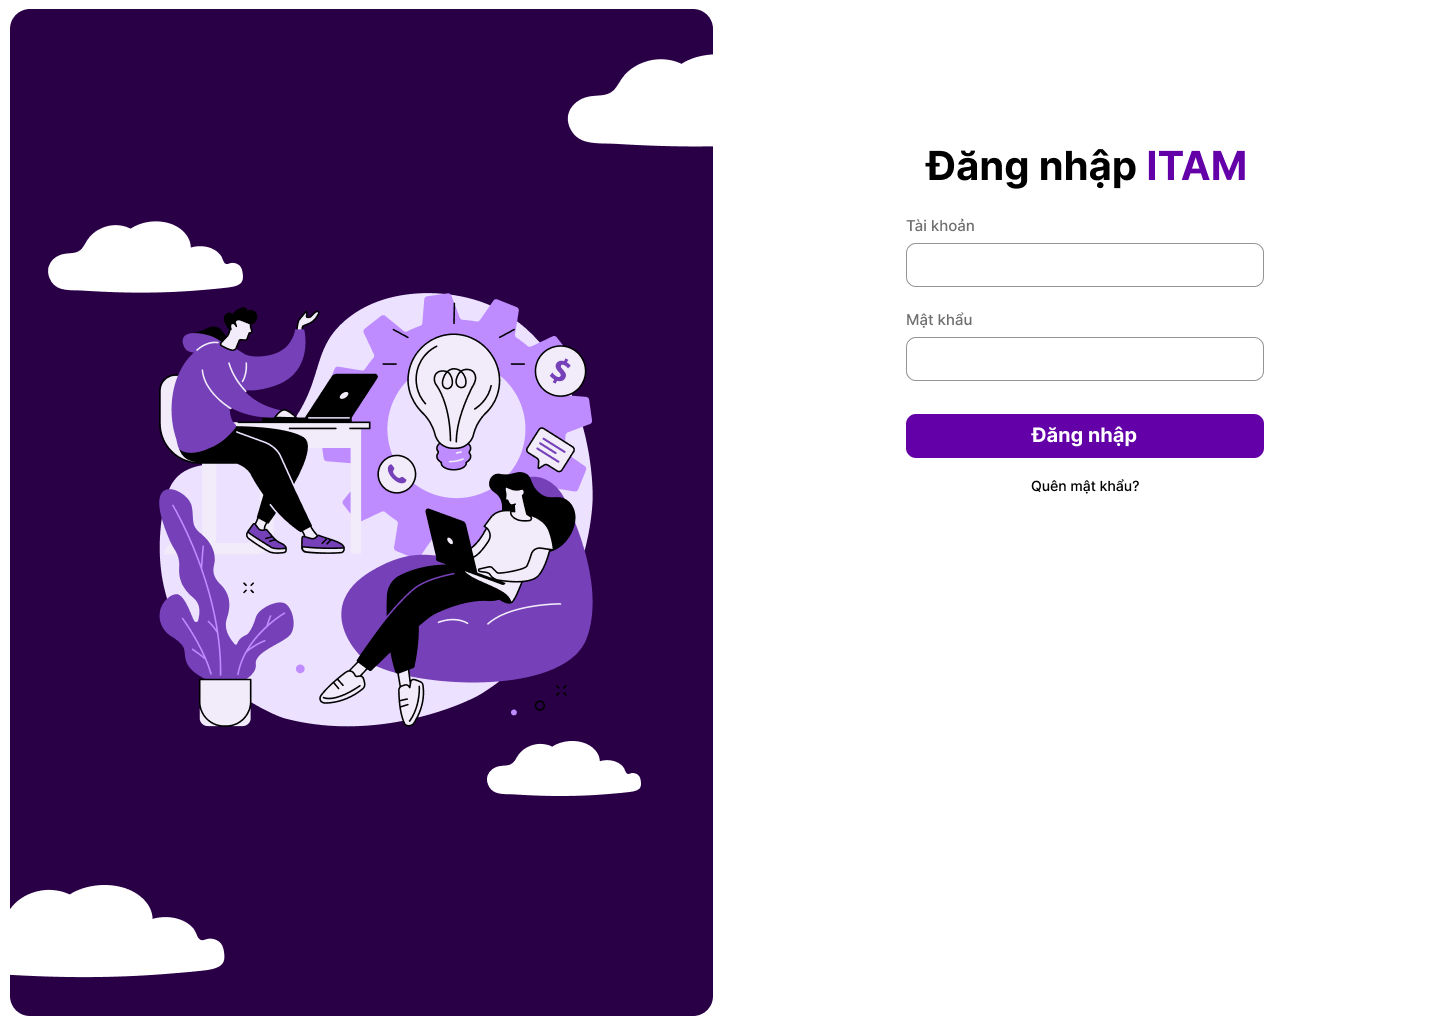
\includegraphics[width=14cm]{Images/C5/UI/Login.png}
%     \vspace{15pt}
%     \caption{Giao diện Đăng nhập}
% \end{figure}

\item{Bảng giám sát}\\
Bảng giám sát thời gian thực hiển thị trạng thái của máy tính có trong hệ thống, giúp nhân viên IT dễ dàng thực hiện giám sát máy tính, xử lý sự cố và cảnh báo một cách kịp thời, đảm bảo hoạt động của các máy tính trong hệ thống. Ngoài ra, tính năng xem tổng quan hoạt động của máy tính trong hệ thống giúp người dùng có cái nhìn tổng quan về hoạt động của các máy tính, cung cấp các thống kê về sự cố và tình trạng máy tính.
\begin{figure}[H]
    \centering
    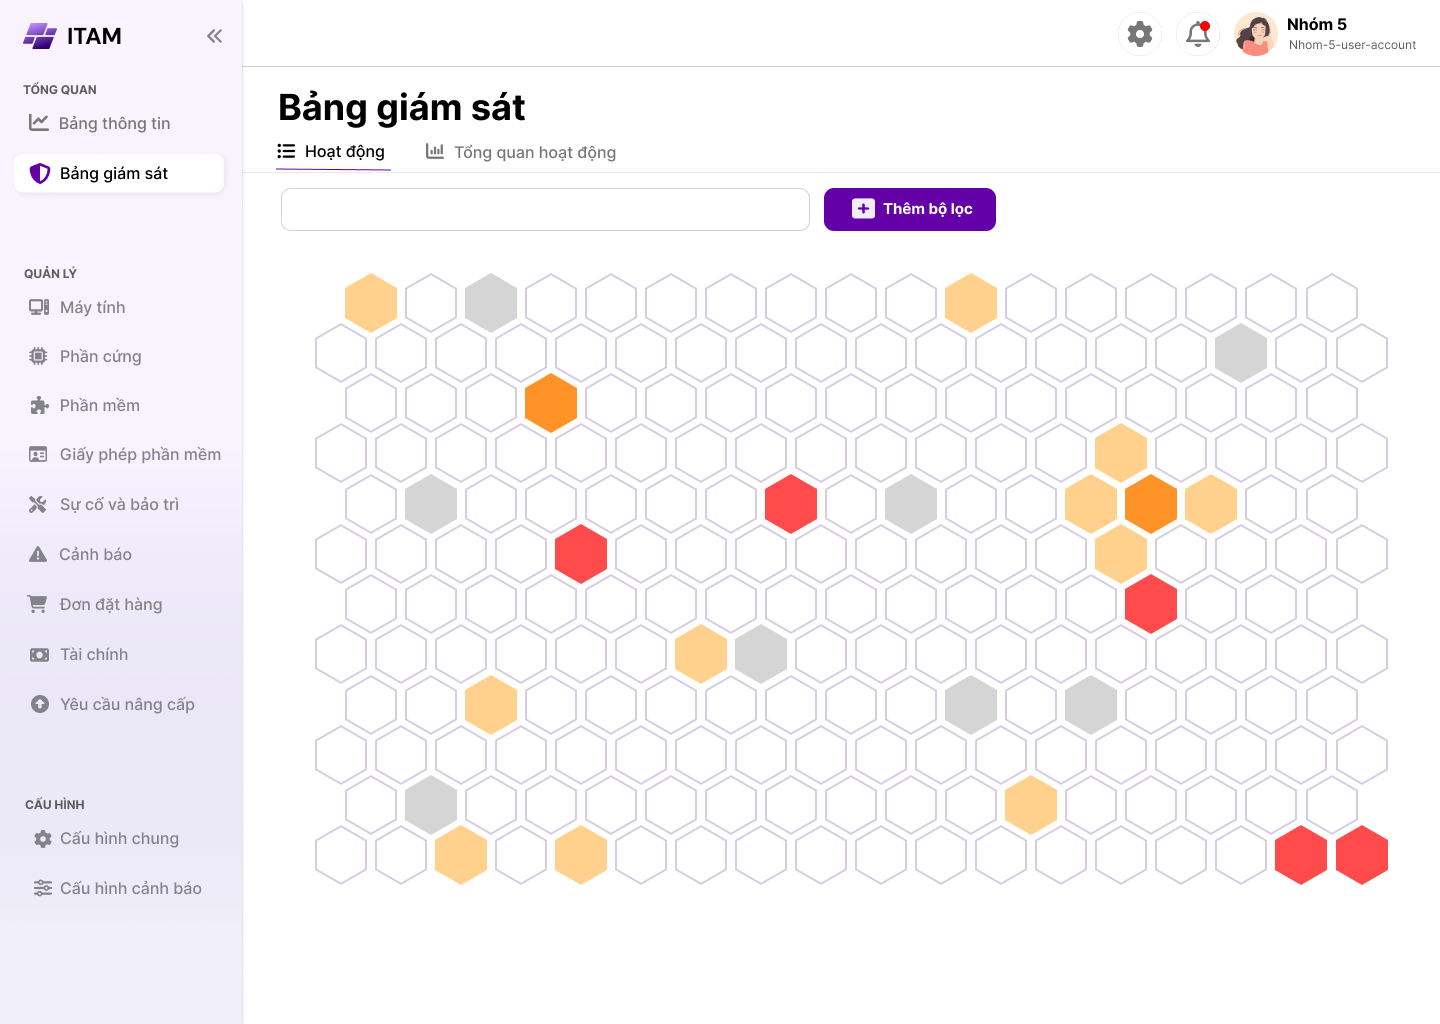
\includegraphics[width=14cm]{Images/C5/UI/Feature-Bảng giám sát 1.1.png}
    \vspace{15pt}
    \caption{Giao diện Bảng giám sát 1}
\end{figure}
% \begin{figure}[H]
%     \centering
%     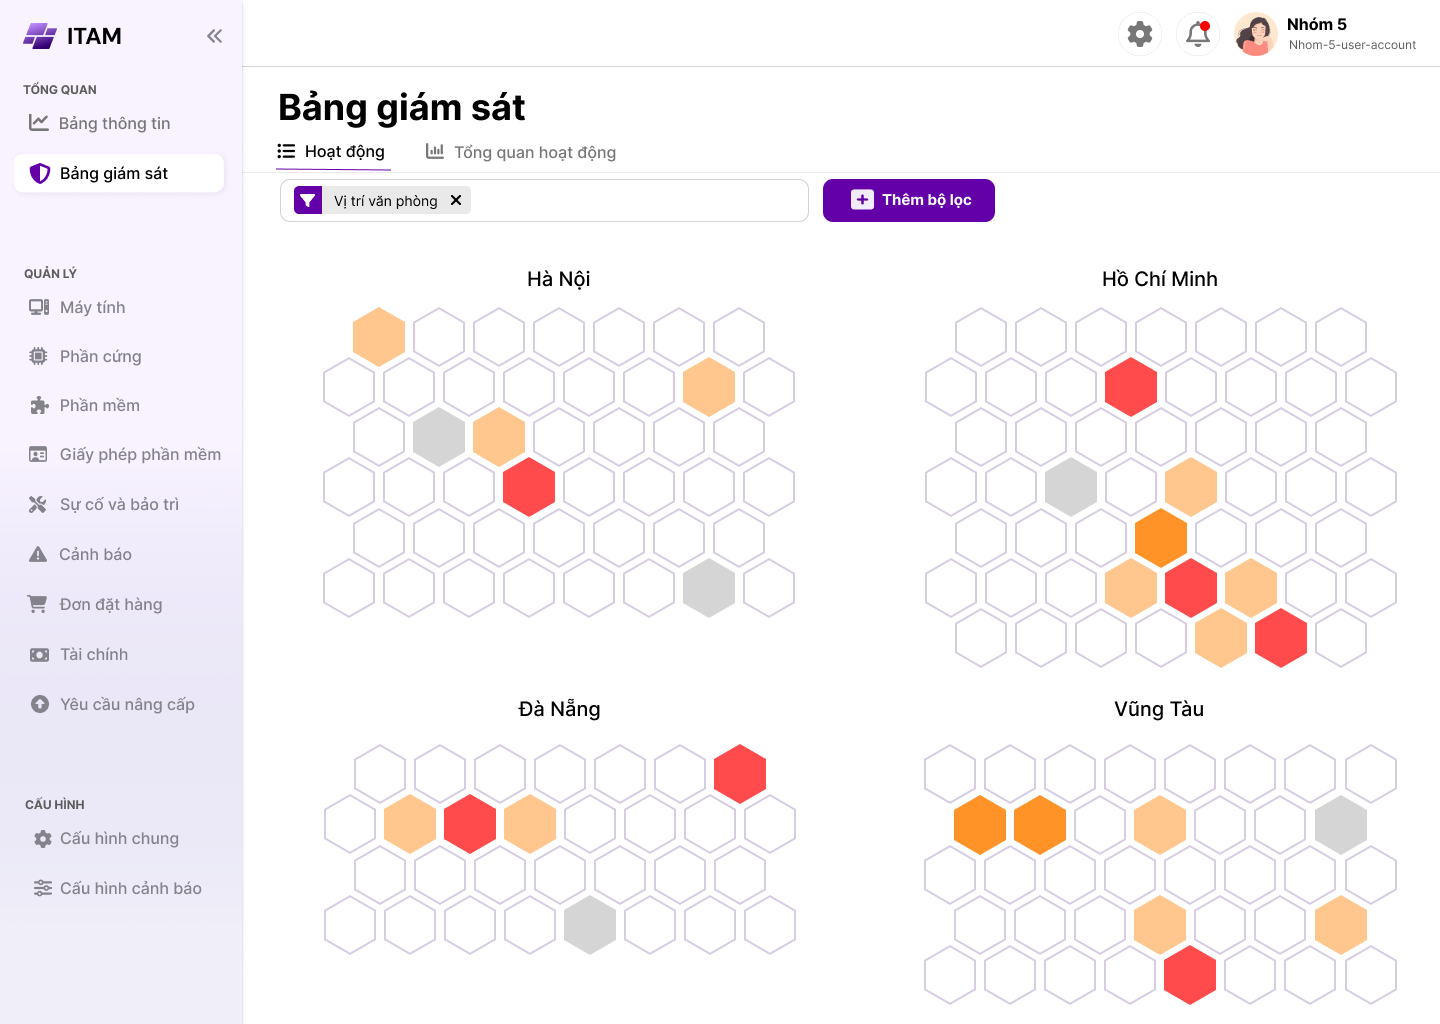
\includegraphics[width=14cm]{Images/C5/UI/Feature-Bảng giám sát 1.2.png}
%     \vspace{15pt}
%     \caption{Giao diện Bảng giám sát 2}
% \end{figure}
% \begin{figure}[H]
%     \centering
%     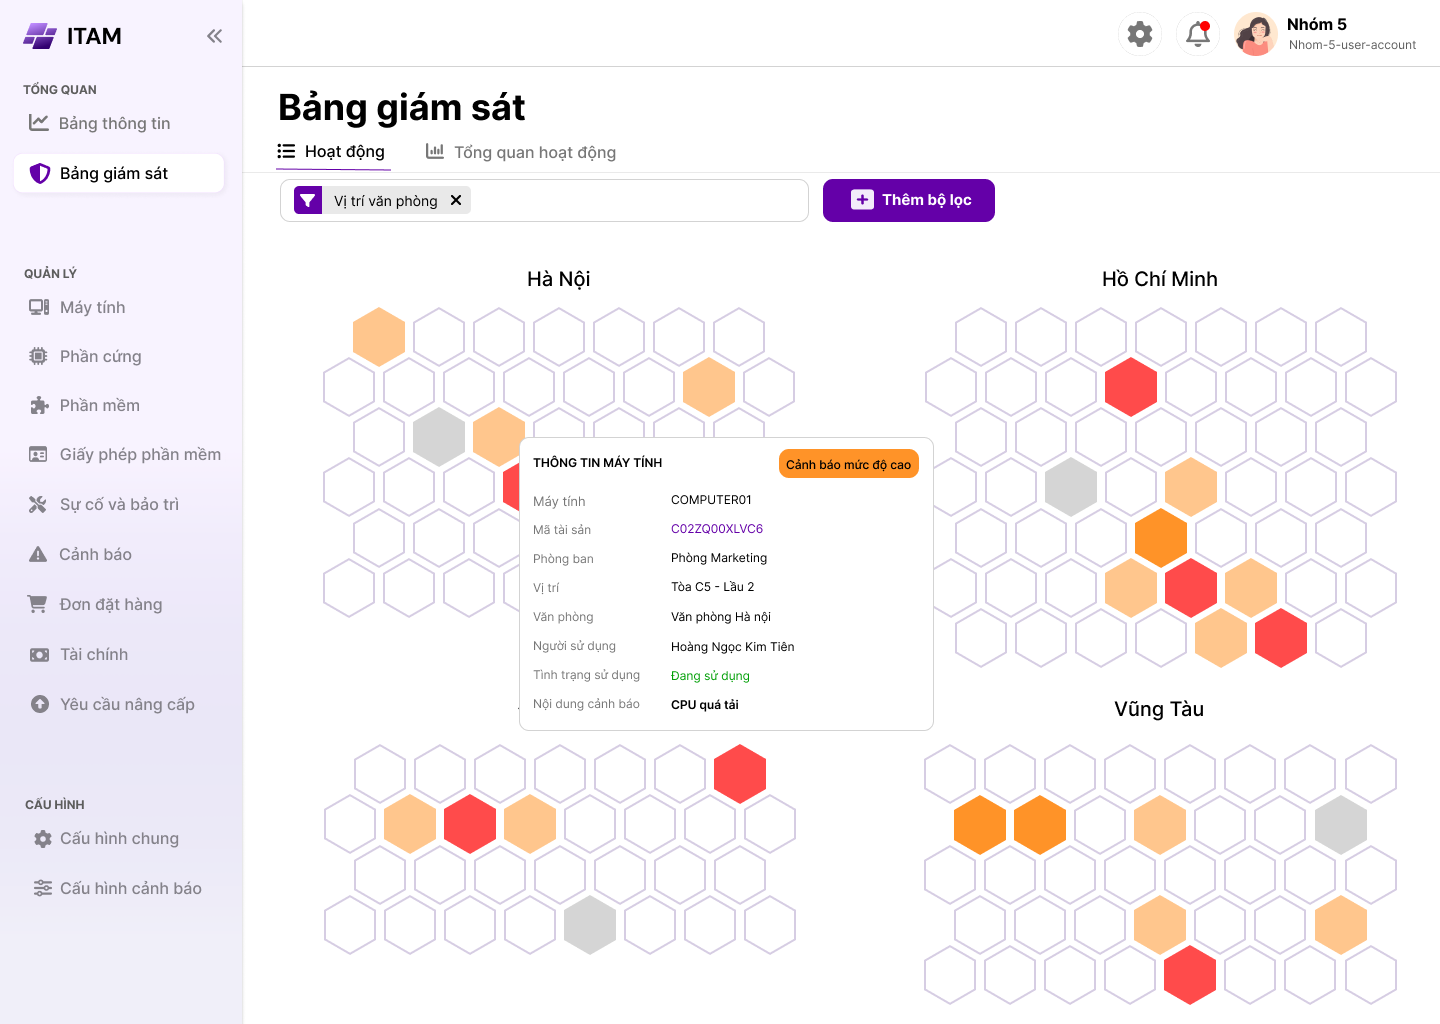
\includegraphics[width=14cm]{Images/C5/UI/Feature-Bảng giám sát 1.3.png}
%     \vspace{15pt}
%     \caption{Giao diện Bảng giám sát 2}
% \end{figure}
% \begin{figure}[H]
%     \centering
%     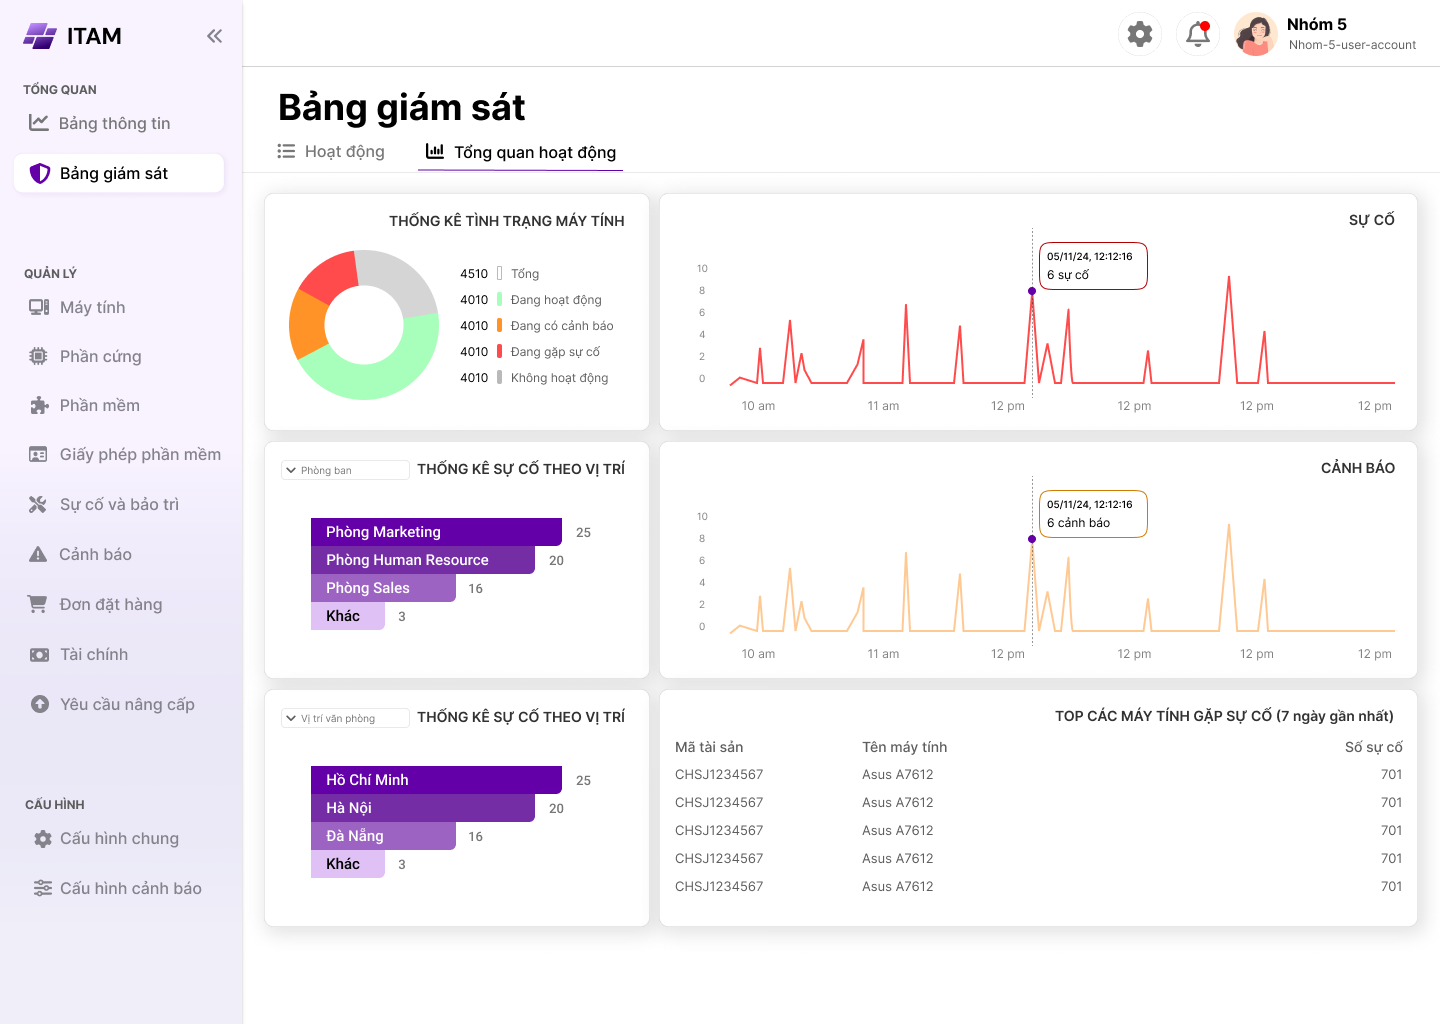
\includegraphics[width=14cm]{Images/C5/UI/Feature-Bảng giám sát 2.png}
%     \vspace{15pt}
%     \caption{Giao diện Bảng giám sát 3}
% \end{figure}

\item{Quản lý máy tính}\\
Quản lý máy tính cung cấp các tính năng cơ bản như xem danh sách máy tính, xem thông tin chi tiết máy tính, chỉnh sửa thông tin chi tiết máy tính, thêm máy tính, gửi yêu cầu nâng cấp, gửi yêu cầu bảo trì, và xem báo cáo tổng quan về máy tính trong hệ thống.\\
Thông tin chi tiết của máy tính gồm:
\begin{itemize}
    \item Thông tin chung như tên, số serial, loại máy tính, địa chỉ MAC,...
    \item Thông tin phần cứng của máy tính
    \item Thông tin phần mềm của máy tính
    \item Thông tin vòng đời của máy tính (Mua sắm, triển khai, sử dung, thanh lý)
    \item Hiệu suất sử dụng
\end{itemize}
% \begin{figure}[H]
%     \centering
%     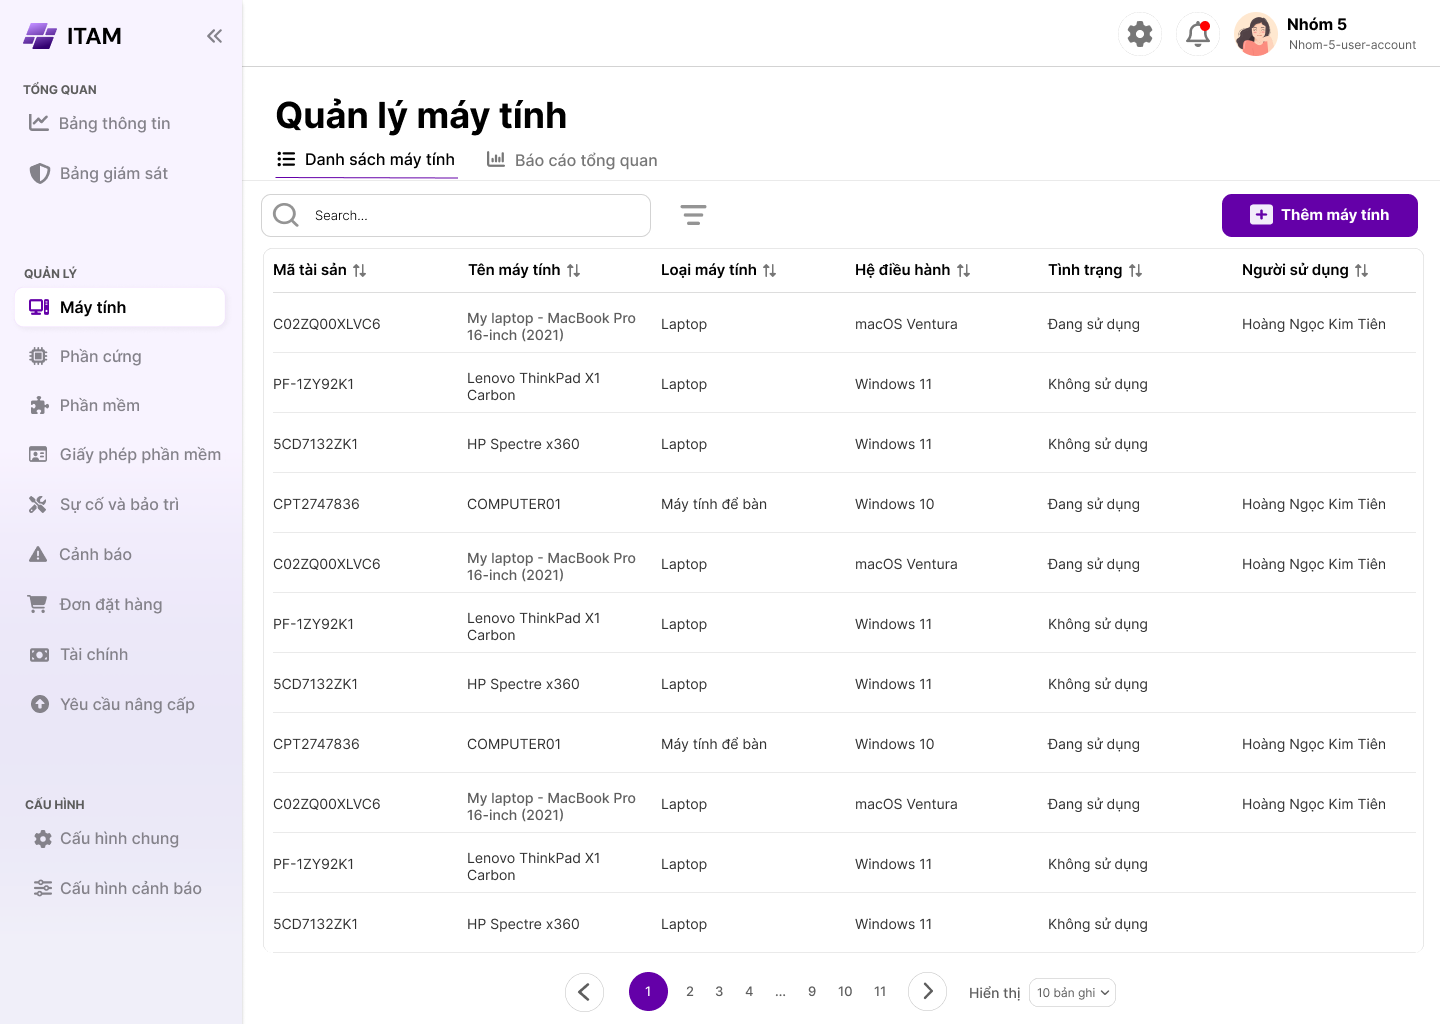
\includegraphics[width=14cm]{Images/C5/UI/Feature-Giám sát tài sản-Máy tính 1.1.png}
%     \vspace{15pt}
%     \caption{Giao diện Quản lý máy tính 1}
% \end{figure}
% \begin{figure}[H]
%     \centering
%     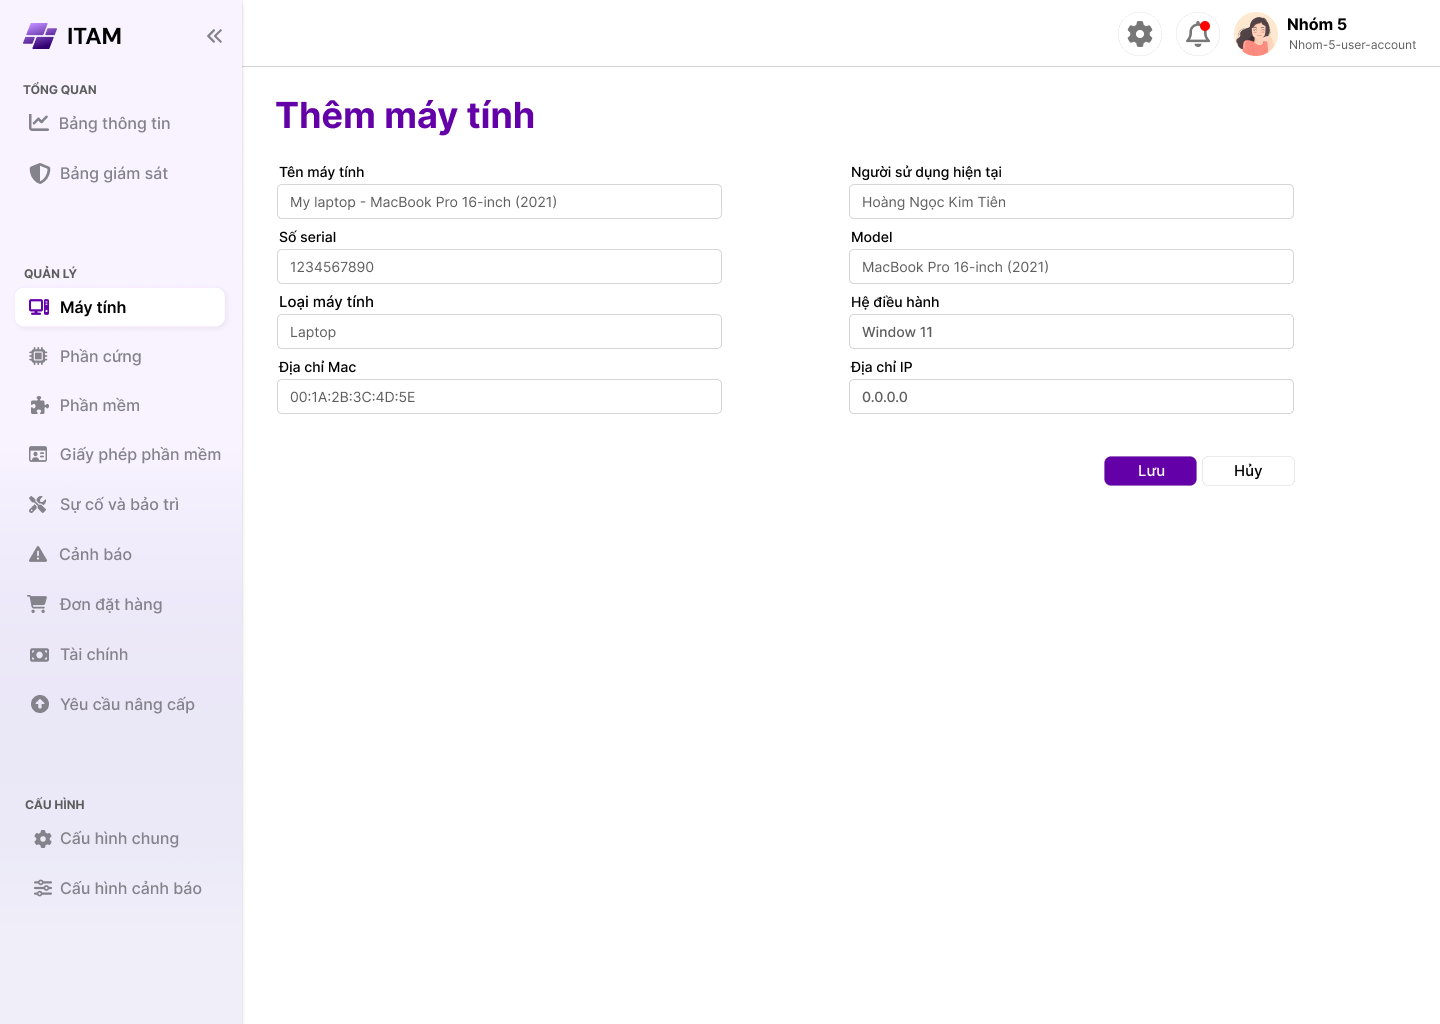
\includegraphics[width=14cm]{Images/C5/UI/Feature-Giám sát tài sản-Máy tính 1.2.png}
%     \vspace{15pt}
%     \caption{Giao diện Quản lý máy tính 2}
% \end{figure}
\begin{figure}[H]
    \centering
    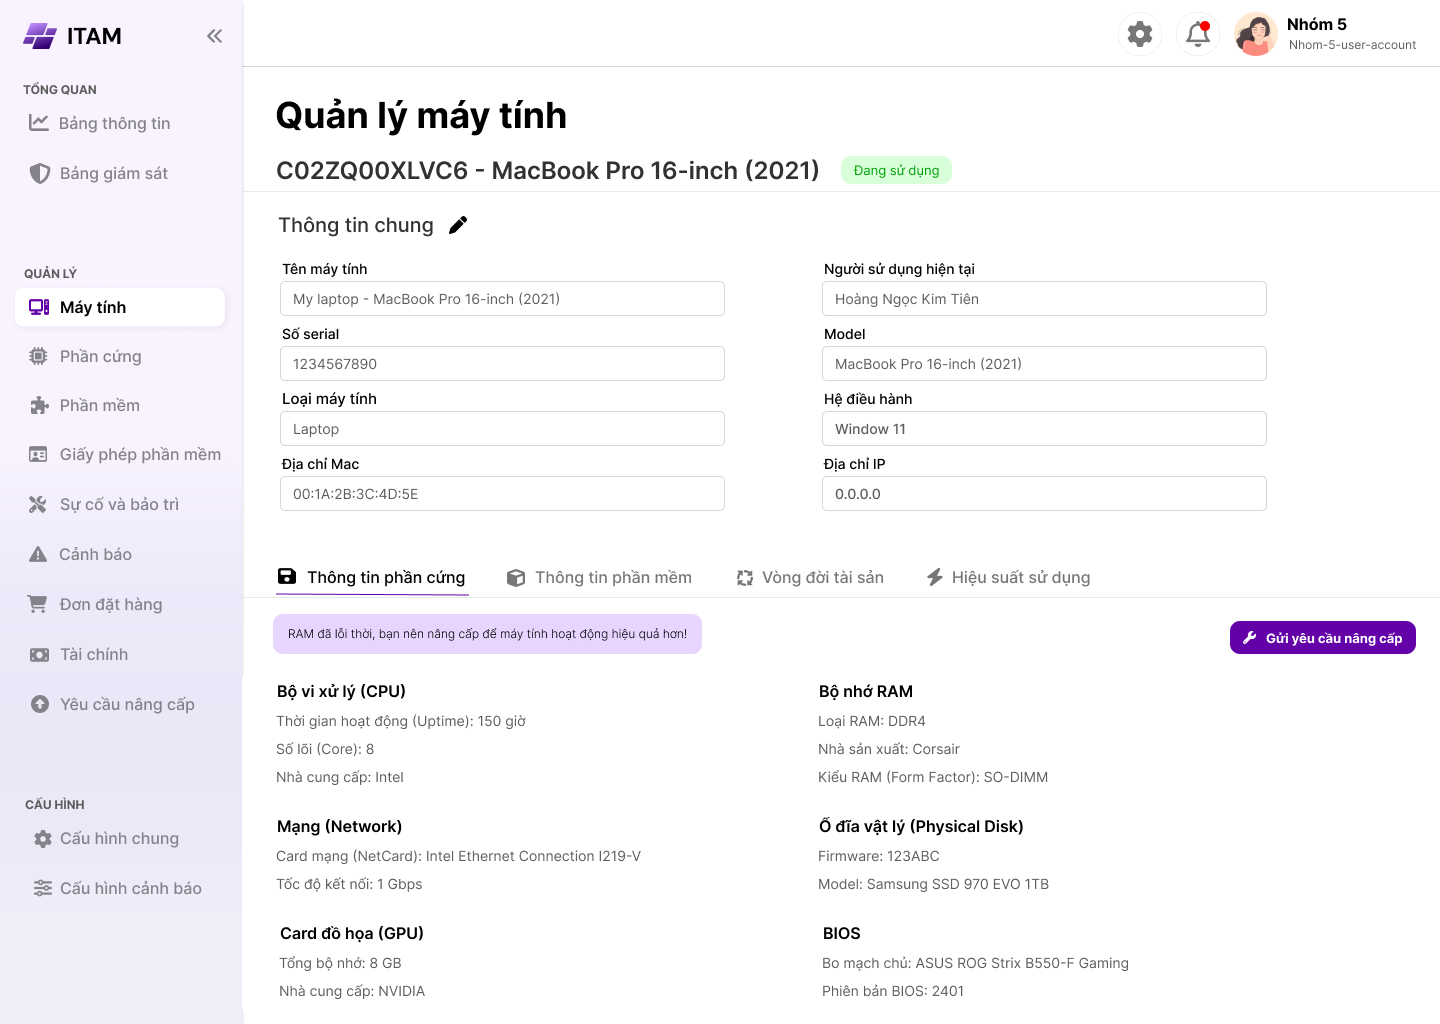
\includegraphics[width=14cm]{Images/C5/UI/Feature-Giám sát tài sản-Máy tính 2.1.png}
    \vspace{15pt}
    \caption{Giao diện Quản lý máy tính 1}
\end{figure}
% \begin{figure}[H]
%     \centering
%     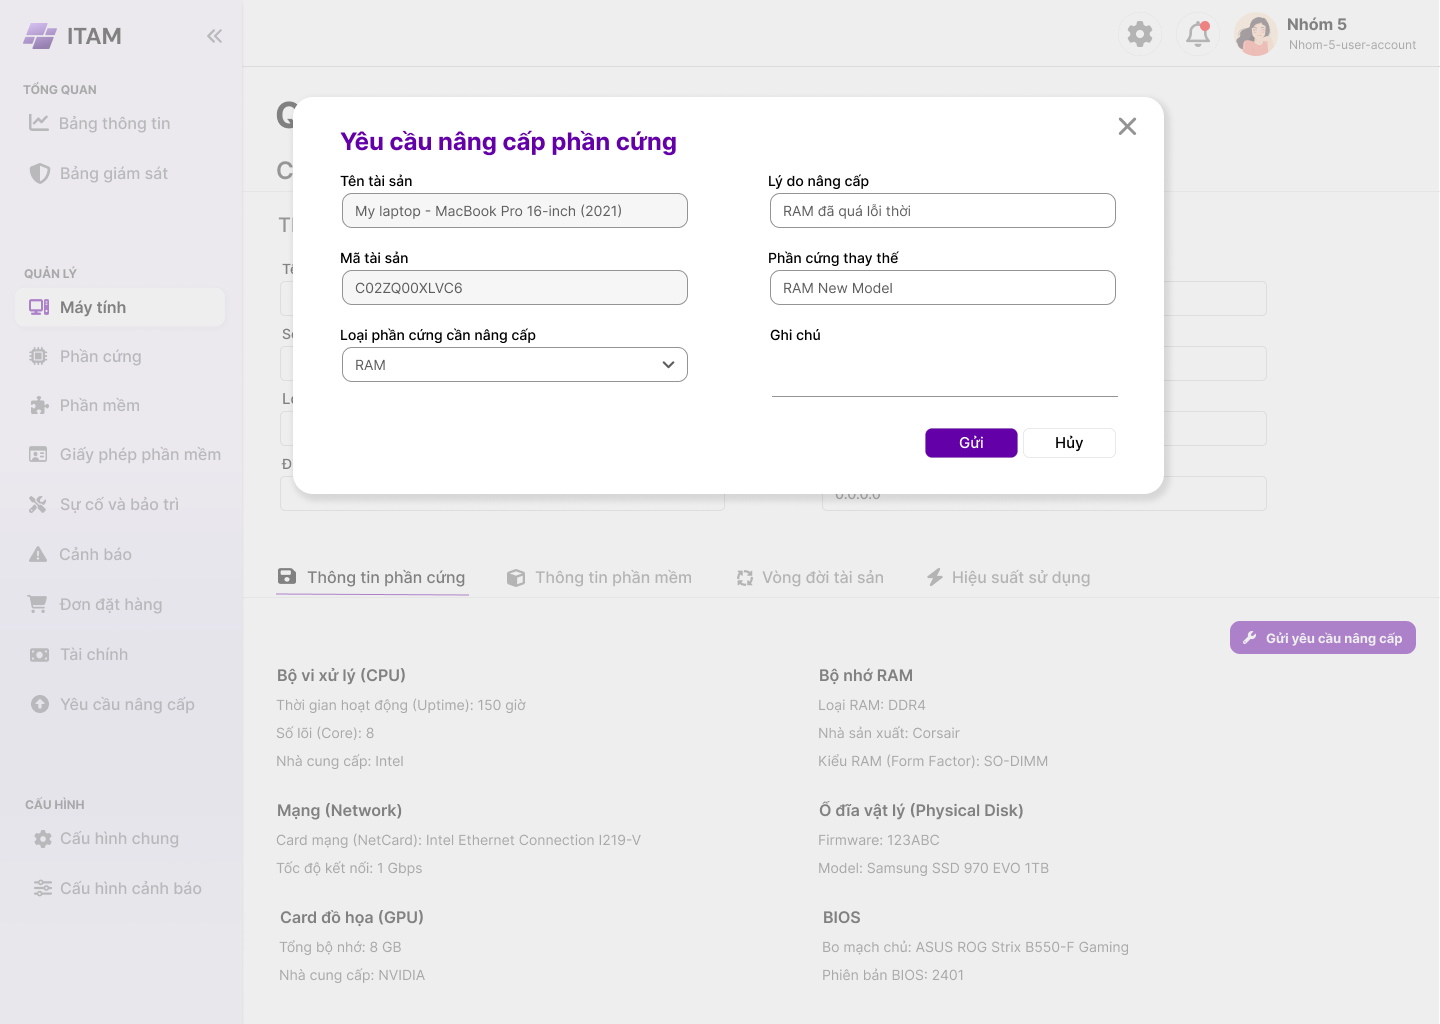
\includegraphics[width=14cm]{Images/C5/UI/Feature-Giám sát tài sản-Máy tính 2.2.png}
%     \vspace{15pt}
%     \caption{Giao diện Quản lý máy tính 4}
% \end{figure}
% \begin{figure}[H]
%     \centering
%     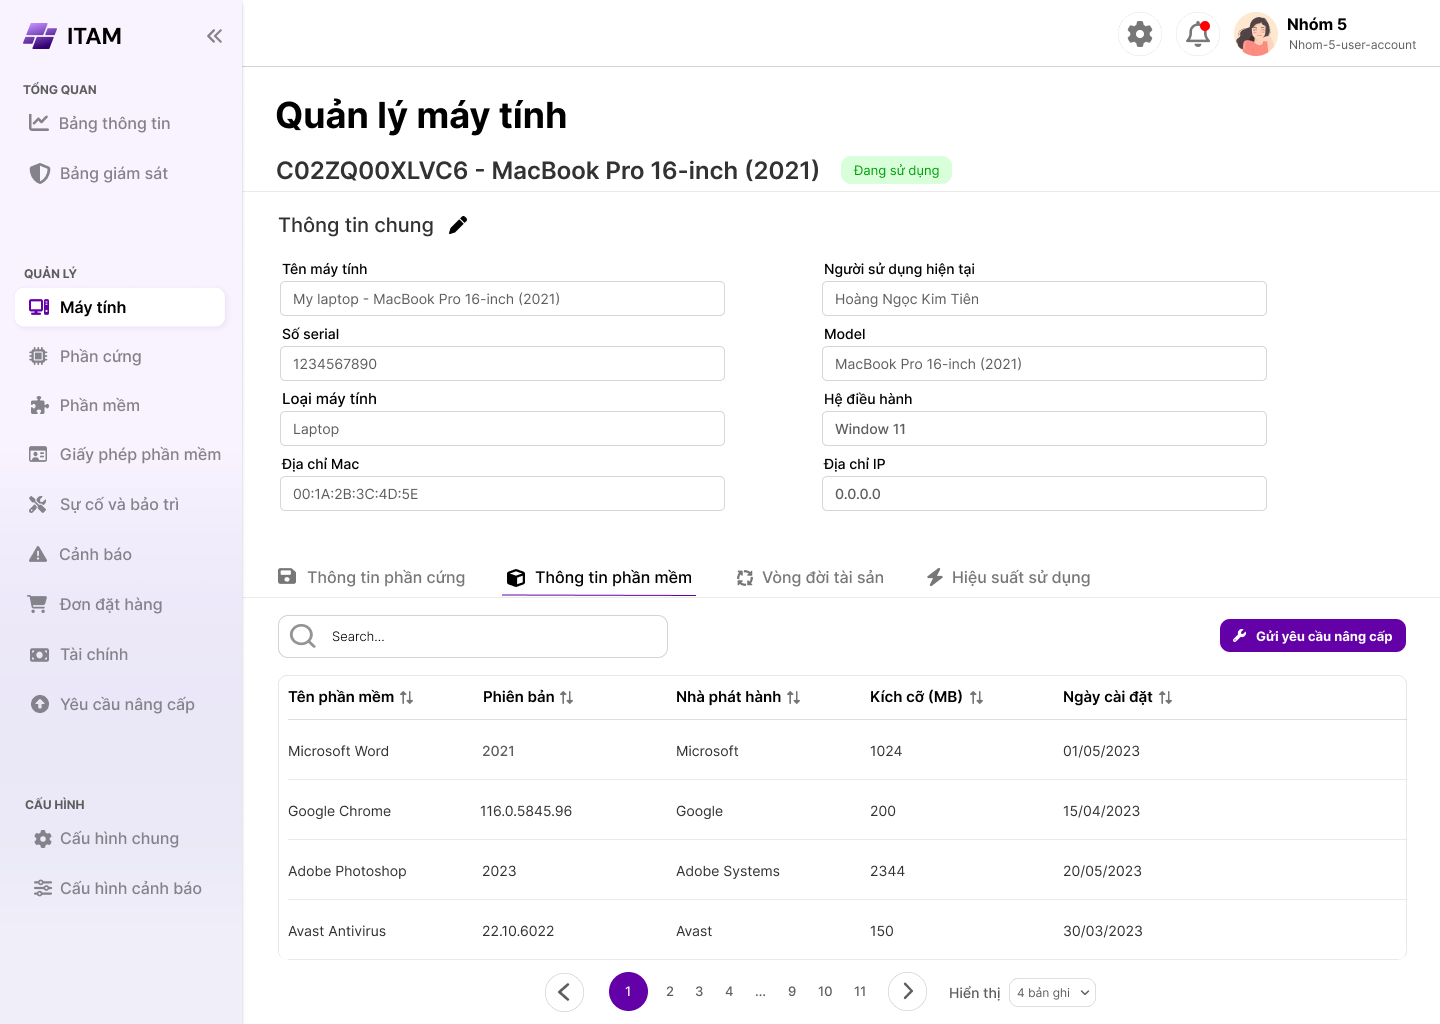
\includegraphics[width=14cm]{Images/C5/UI/Feature-Giám sát tài sản-Máy tính 3.1.png}
%     \vspace{15pt}
%     \caption{Giao diện Quản lý máy tính 5}
% \end{figure}
% \begin{figure}[H]
%     \centering
%     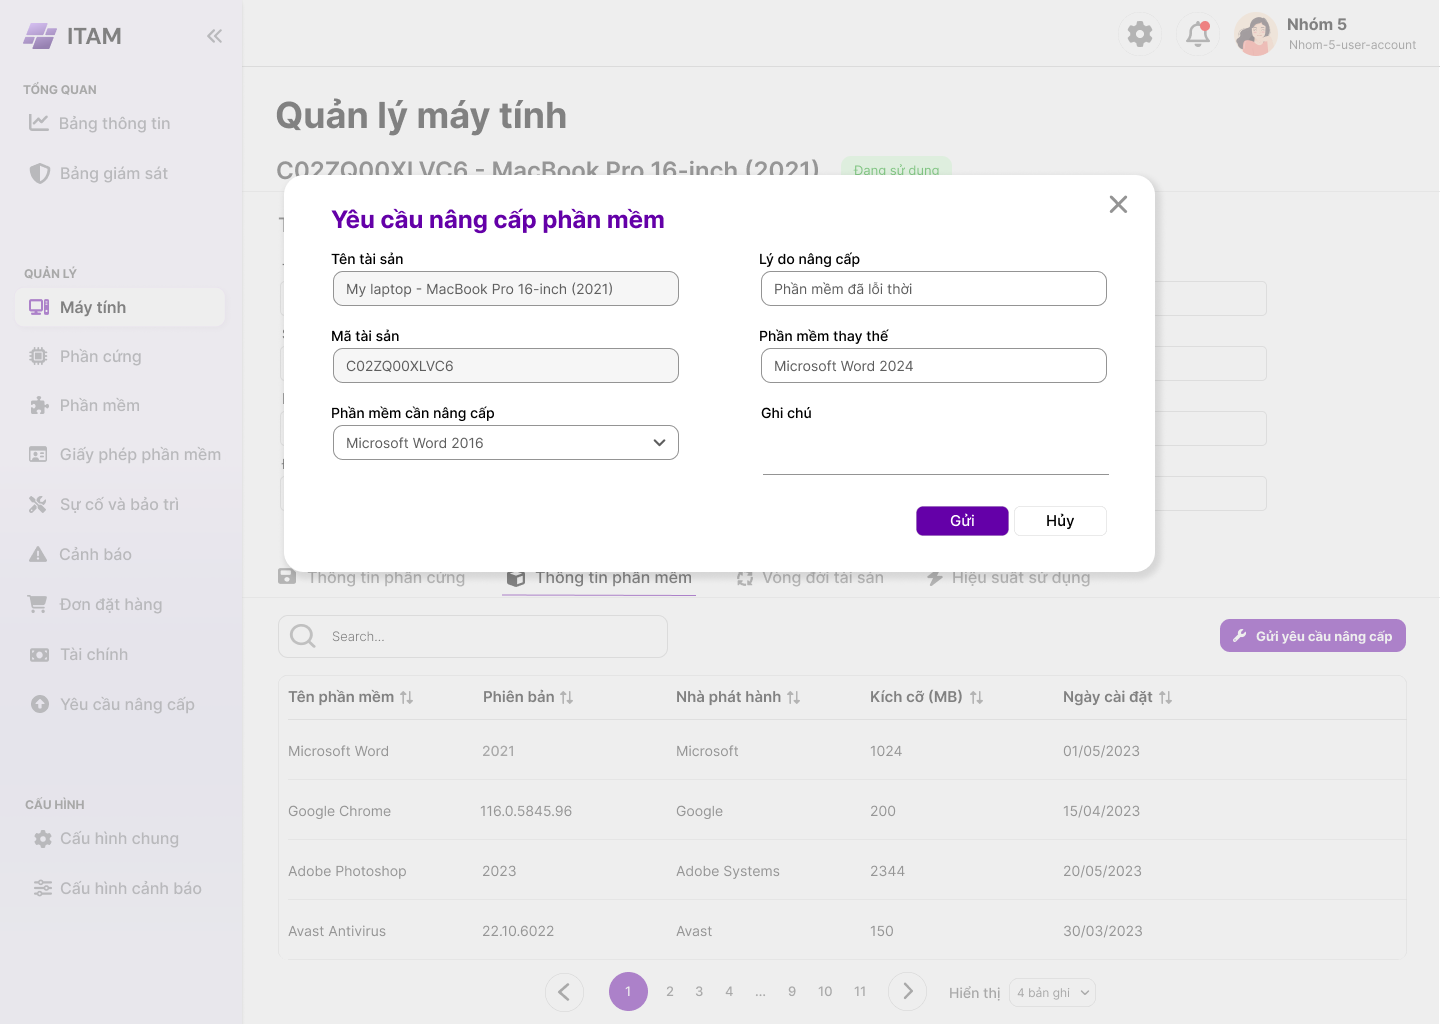
\includegraphics[width=14cm]{Images/C5/UI/Feature-Giám sát tài sản-Máy tính 3.2.png}
%     \vspace{15pt}
%     \caption{Giao diện Quản lý máy tính 6}
% \end{figure}
% \begin{figure}[H]
%     \centering
%     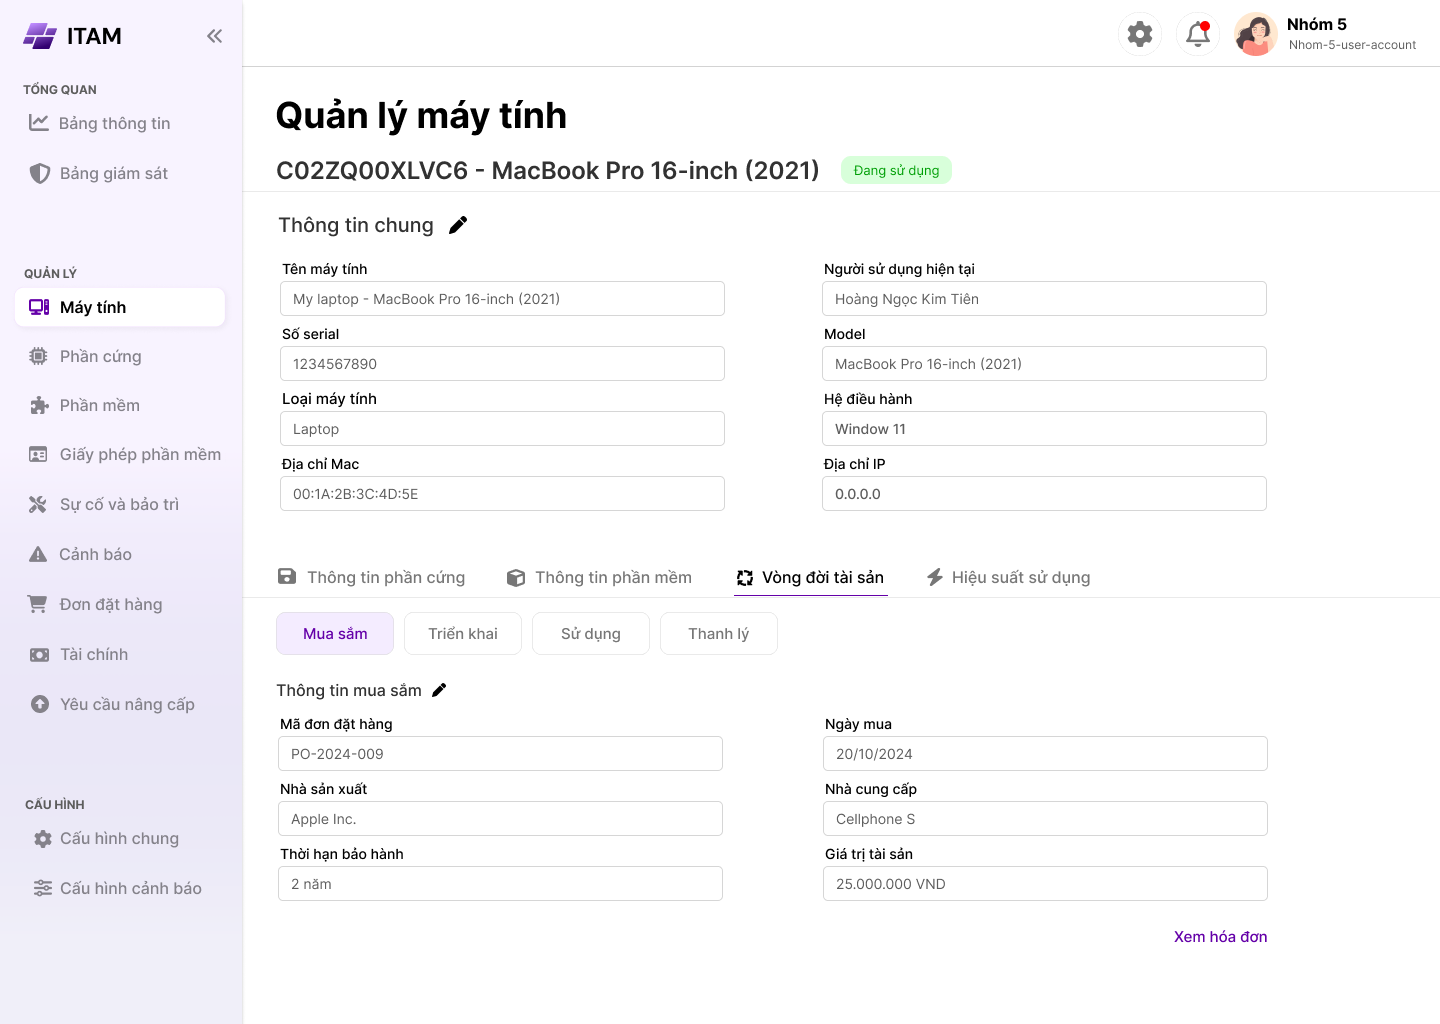
\includegraphics[width=14cm]{Images/C5/UI/Feature-Giám sát tài sản-Máy tính 4.1.png}
%     \vspace{15pt}
%     \caption{Giao diện Quản lý máy tính 7}
% \end{figure}
% \begin{figure}[H]
%     \centering
%     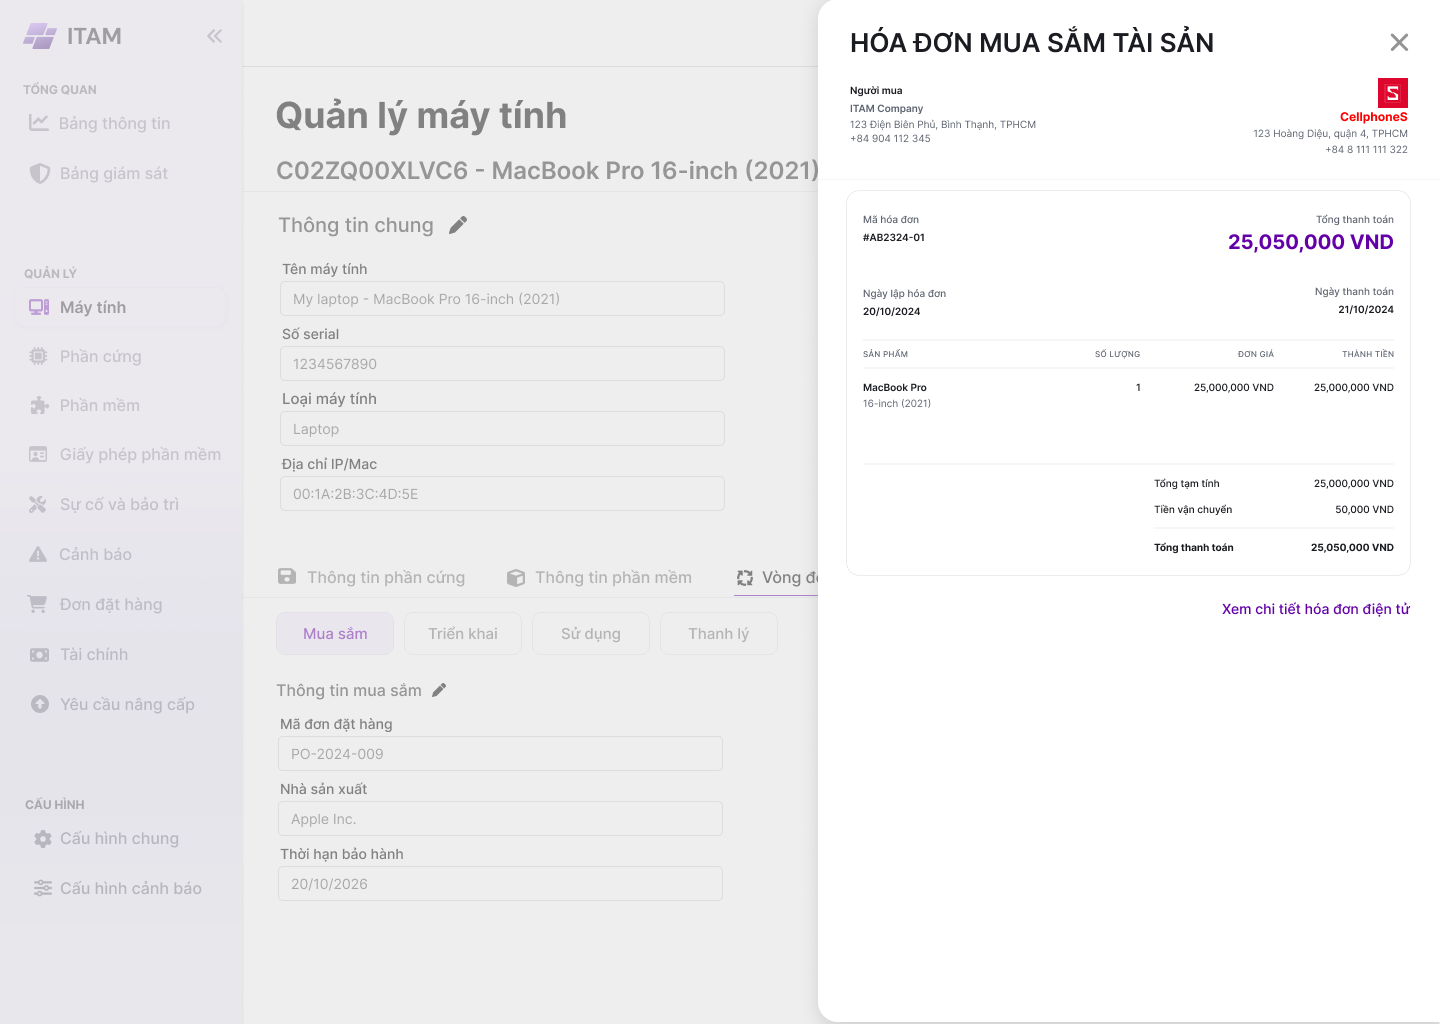
\includegraphics[width=14cm]{Images/C5/UI/Feature-Giám sát tài sản-Máy tính 4.2.png}
%     \vspace{15pt}
%     \caption{Giao diện Quản lý máy tính 8}
% \end{figure}
% \begin{figure}[H]
%     \centering
%     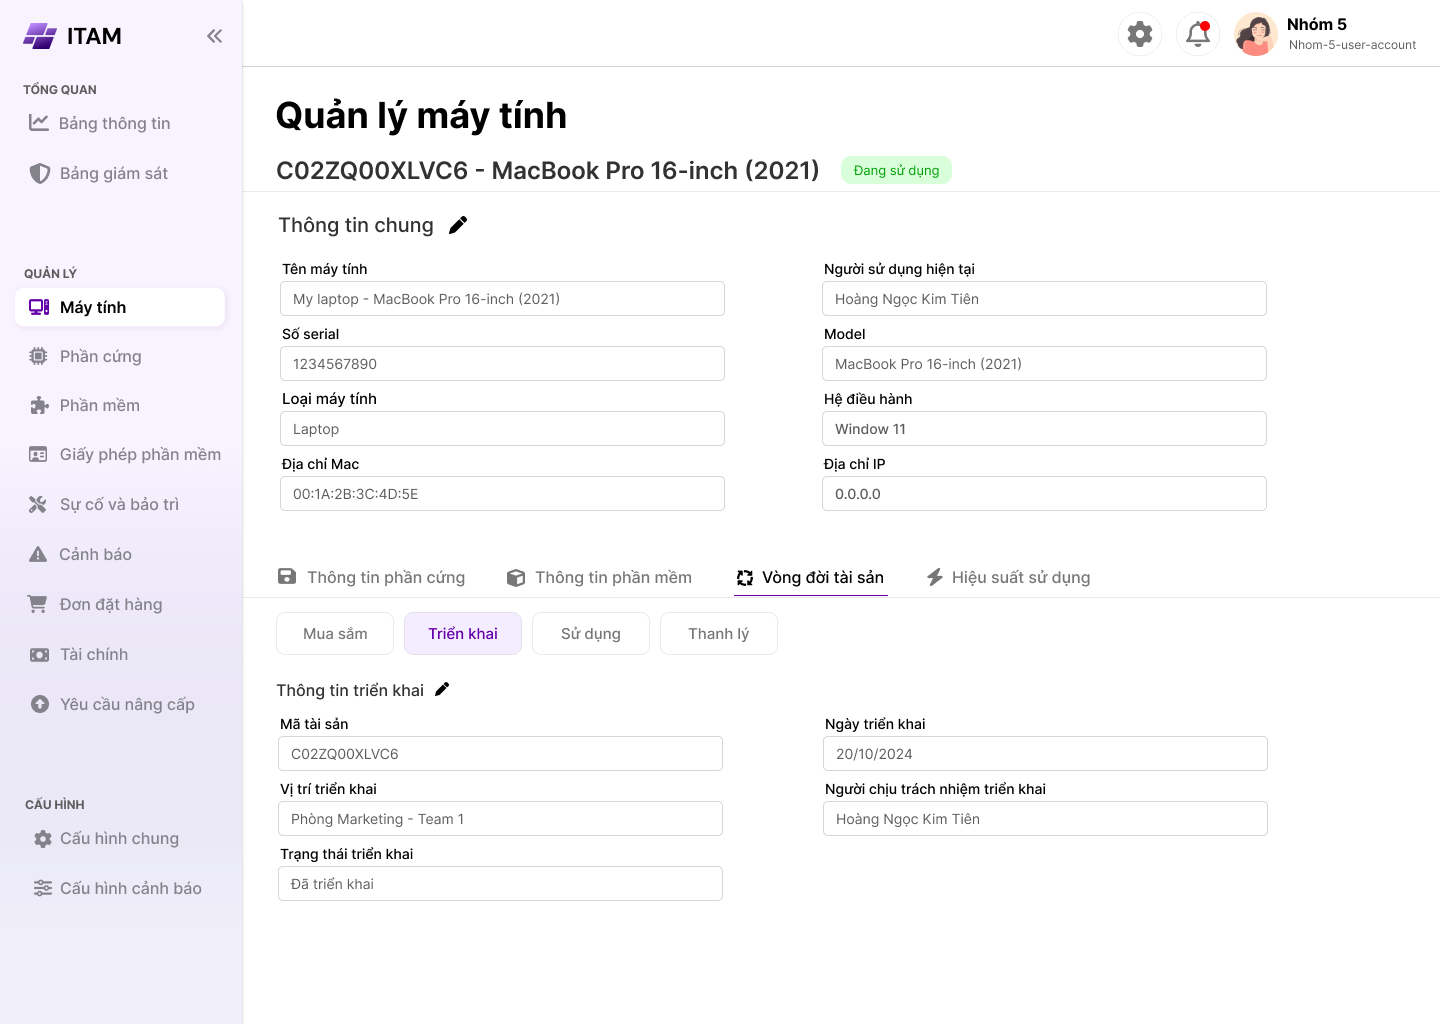
\includegraphics[width=14cm]{Images/C5/UI/Feature-Giám sát tài sản-Máy tính 5.png}
%     \vspace{15pt}
%     \caption{Giao diện Quản lý máy tính 8}
% \end{figure}
% \begin{figure}[H]
%     \centering
%     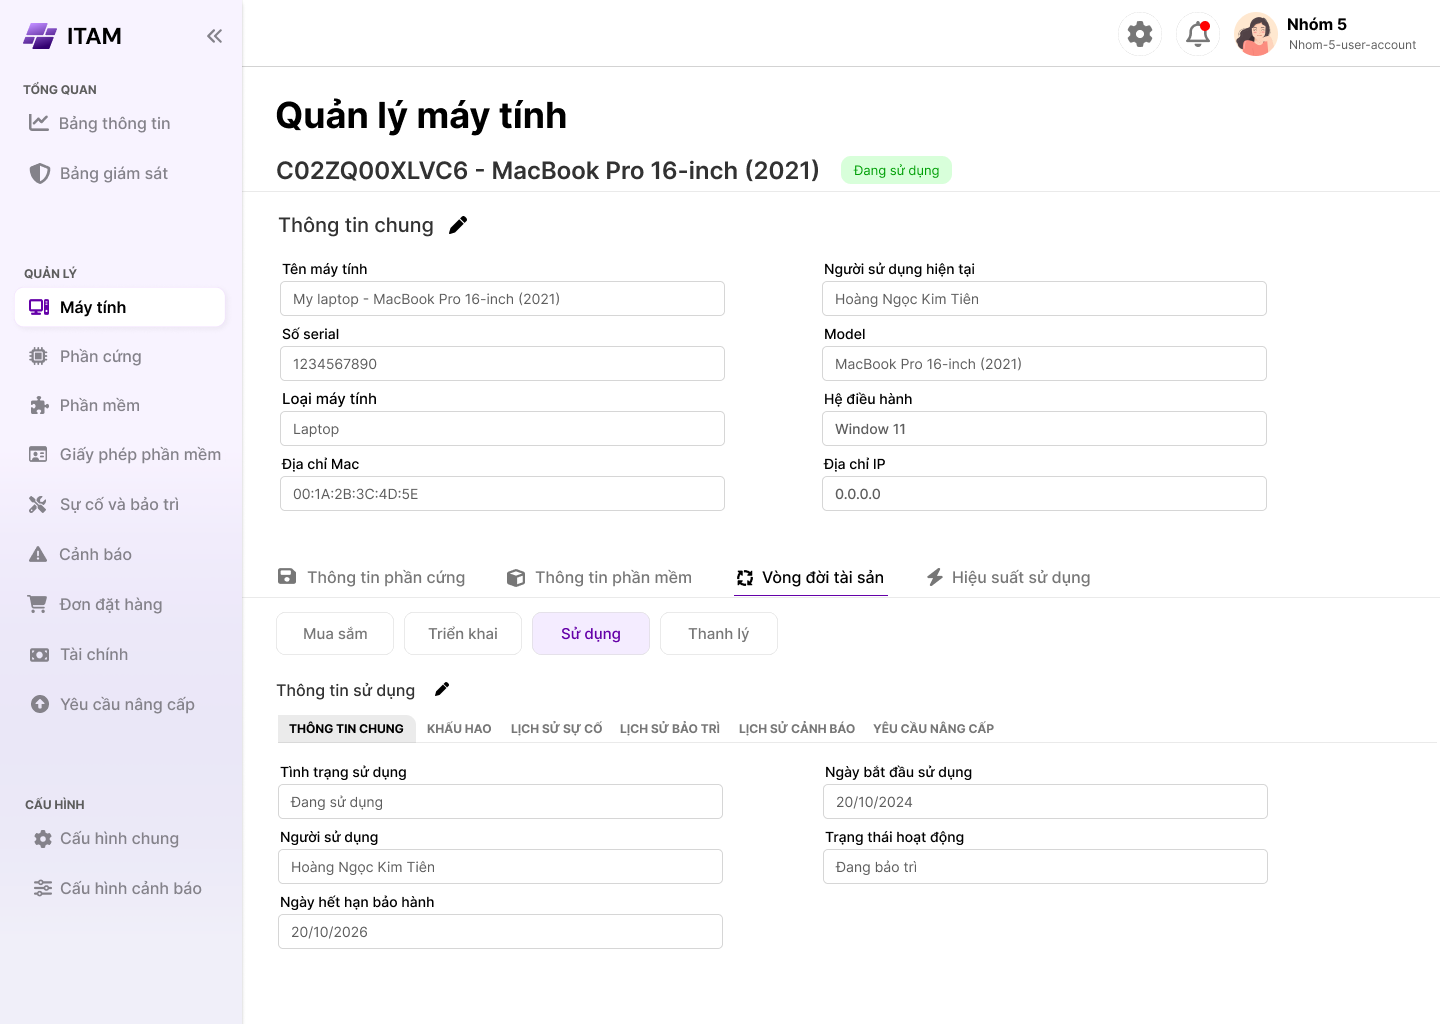
\includegraphics[width=14cm]{Images/C5/UI/Feature-Giám sát tài sản-Máy tính 6.1.png}
%     \vspace{15pt}
%     \caption{Giao diện Quản lý máy tính 9}
% \end{figure}
% \begin{figure}[H]
%     \centering
%     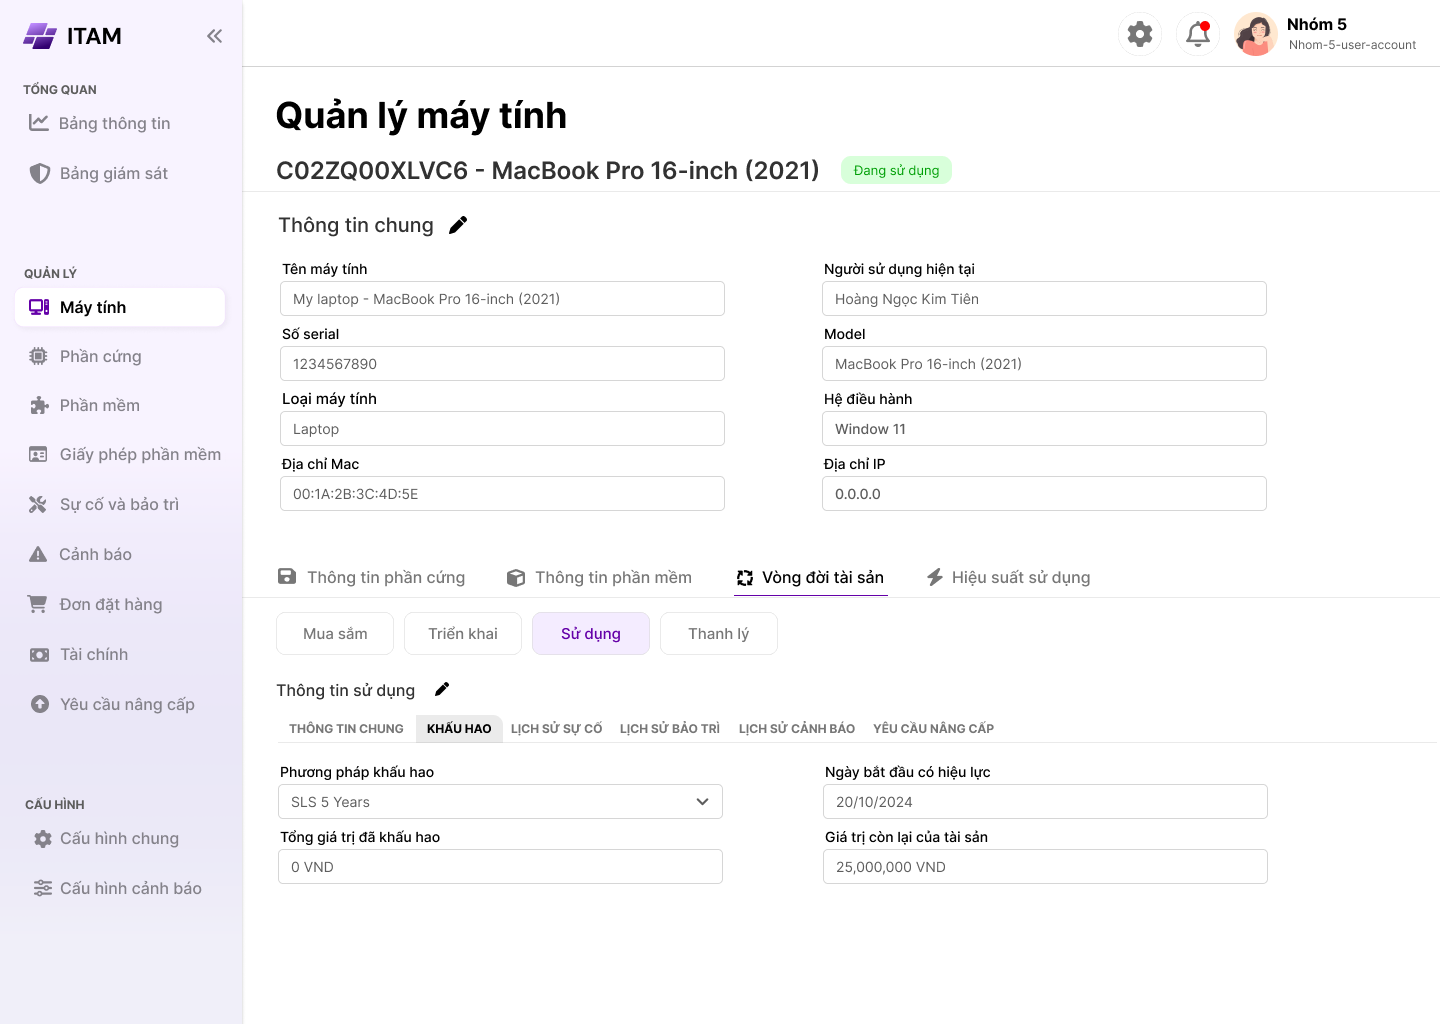
\includegraphics[width=14cm]{Images/C5/UI/Feature-Giám sát tài sản-Máy tính 6.2.png}
%     \vspace{15pt}
%     \caption{Giao diện Quản lý máy tính 11}
% \end{figure}
% \begin{figure}[H]
%     \centering
%     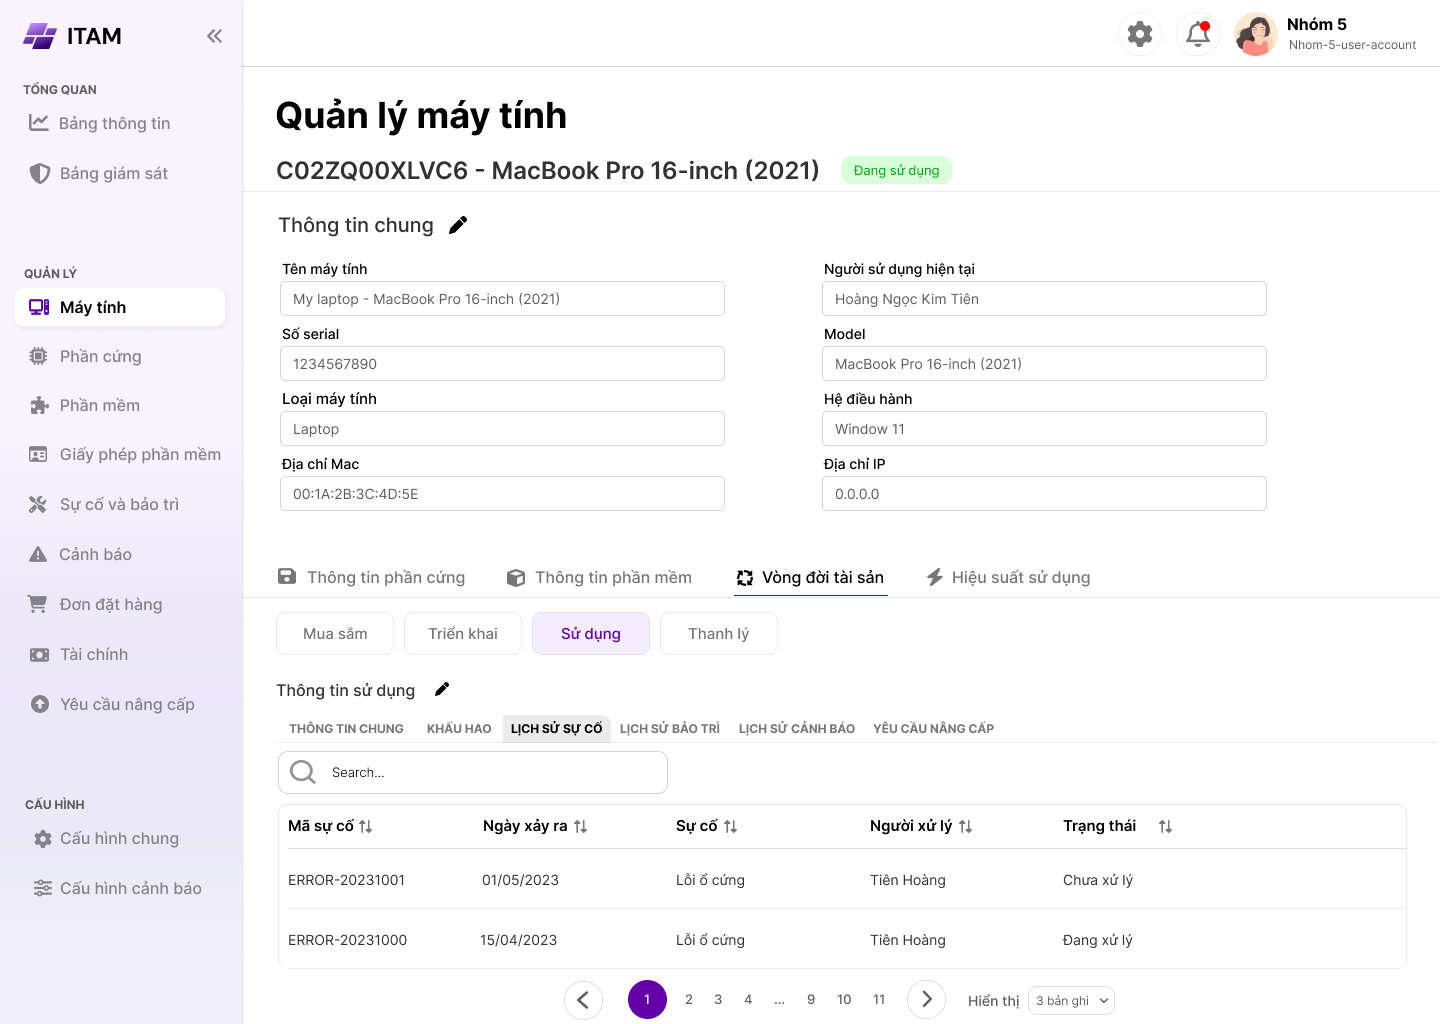
\includegraphics[width=14cm]{Images/C5/UI/Feature-Giám sát tài sản-Máy tính 6.3.png}
%     \vspace{15pt}
%     \caption{Giao diện Quản lý máy tính 12}
% \end{figure}
% \begin{figure}[H]
%     \centering
%     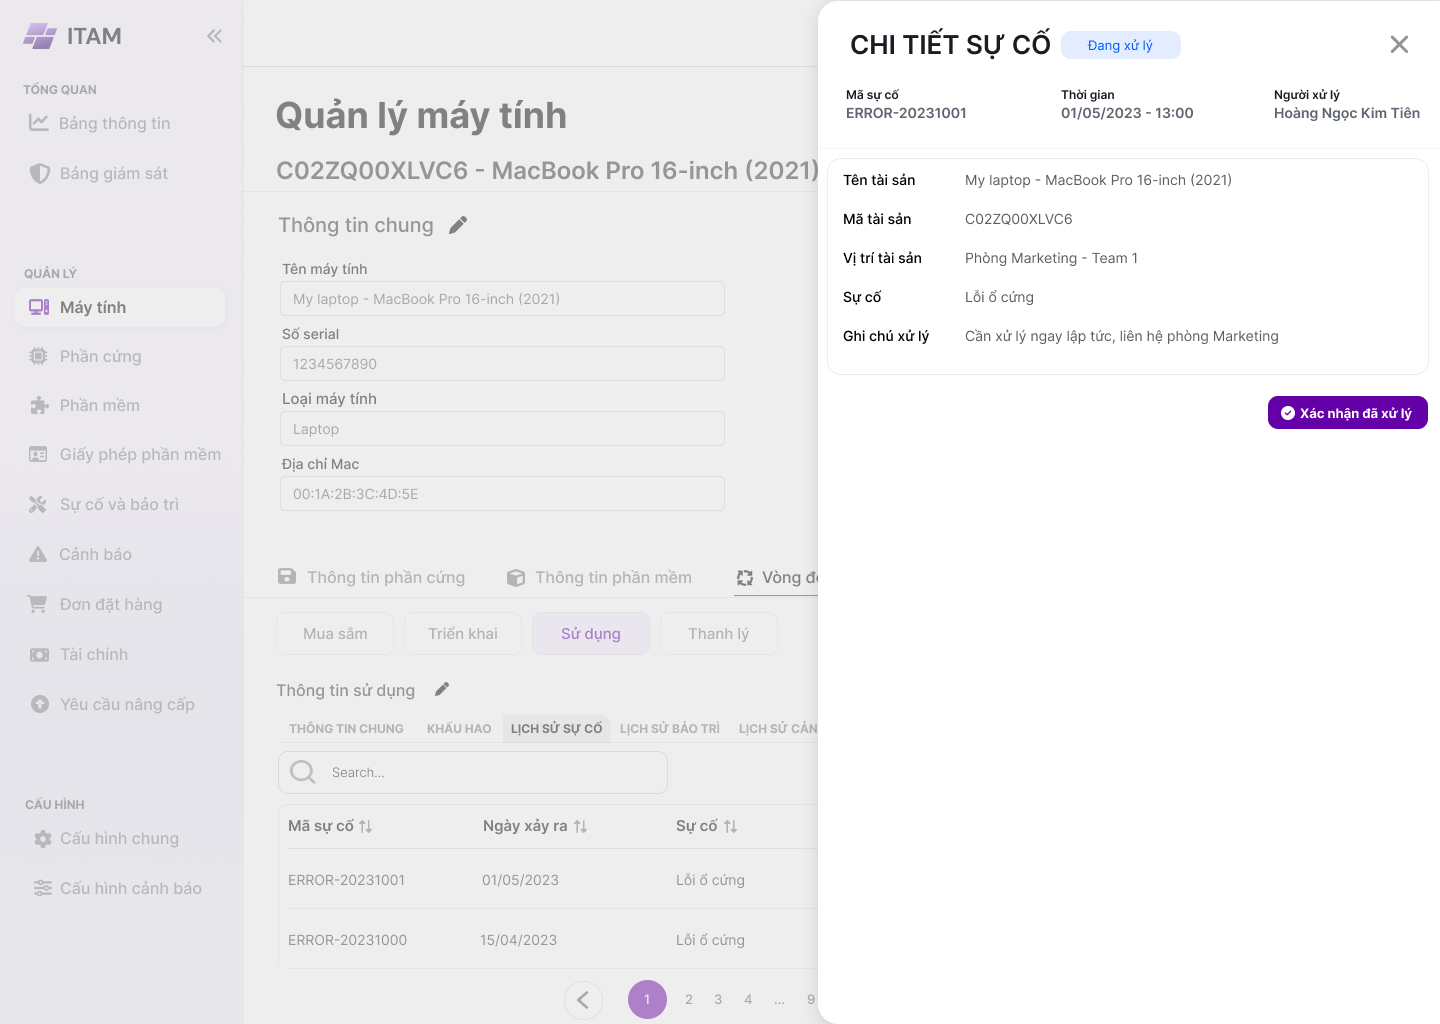
\includegraphics[width=14cm]{Images/C5/UI/Feature-Giám sát tài sản-Máy tính 6.4.png}
%     \vspace{15pt}
%     \caption{Giao diện Quản lý máy tính 13}
% \end{figure}
% \begin{figure}[H]
%     \centering
%     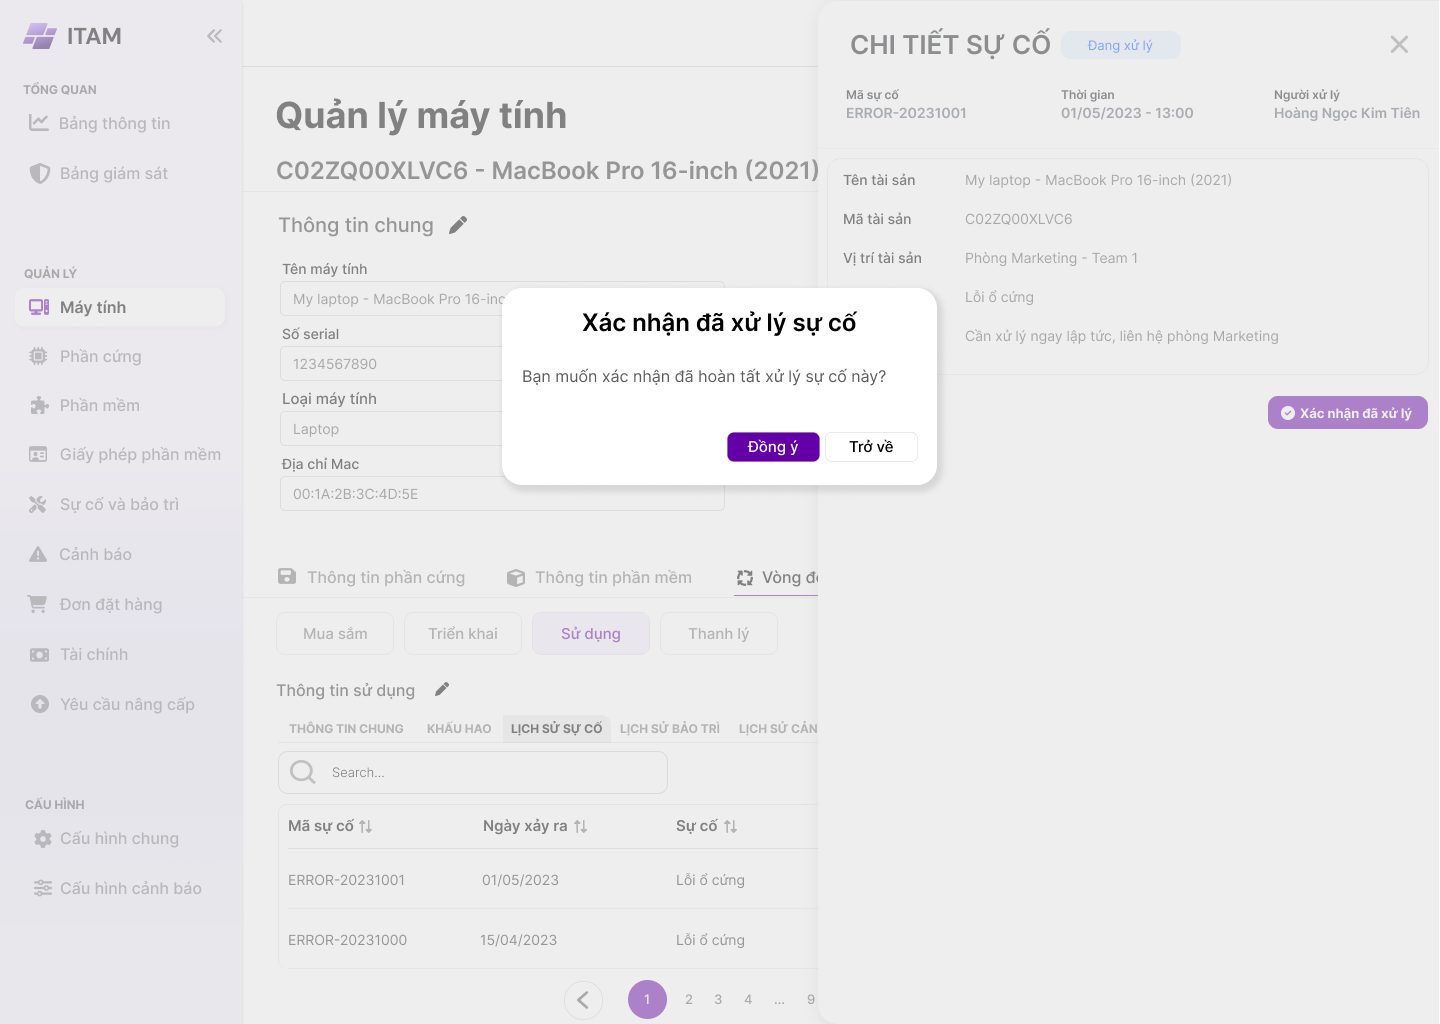
\includegraphics[width=14cm]{Images/C5/UI/Feature-Giám sát tài sản-Máy tính 6.5.png}
%     \vspace{15pt}
%     \caption{Giao diện Quản lý máy tính 14}
% \end{figure}
% \begin{figure}[H]
%     \centering
%     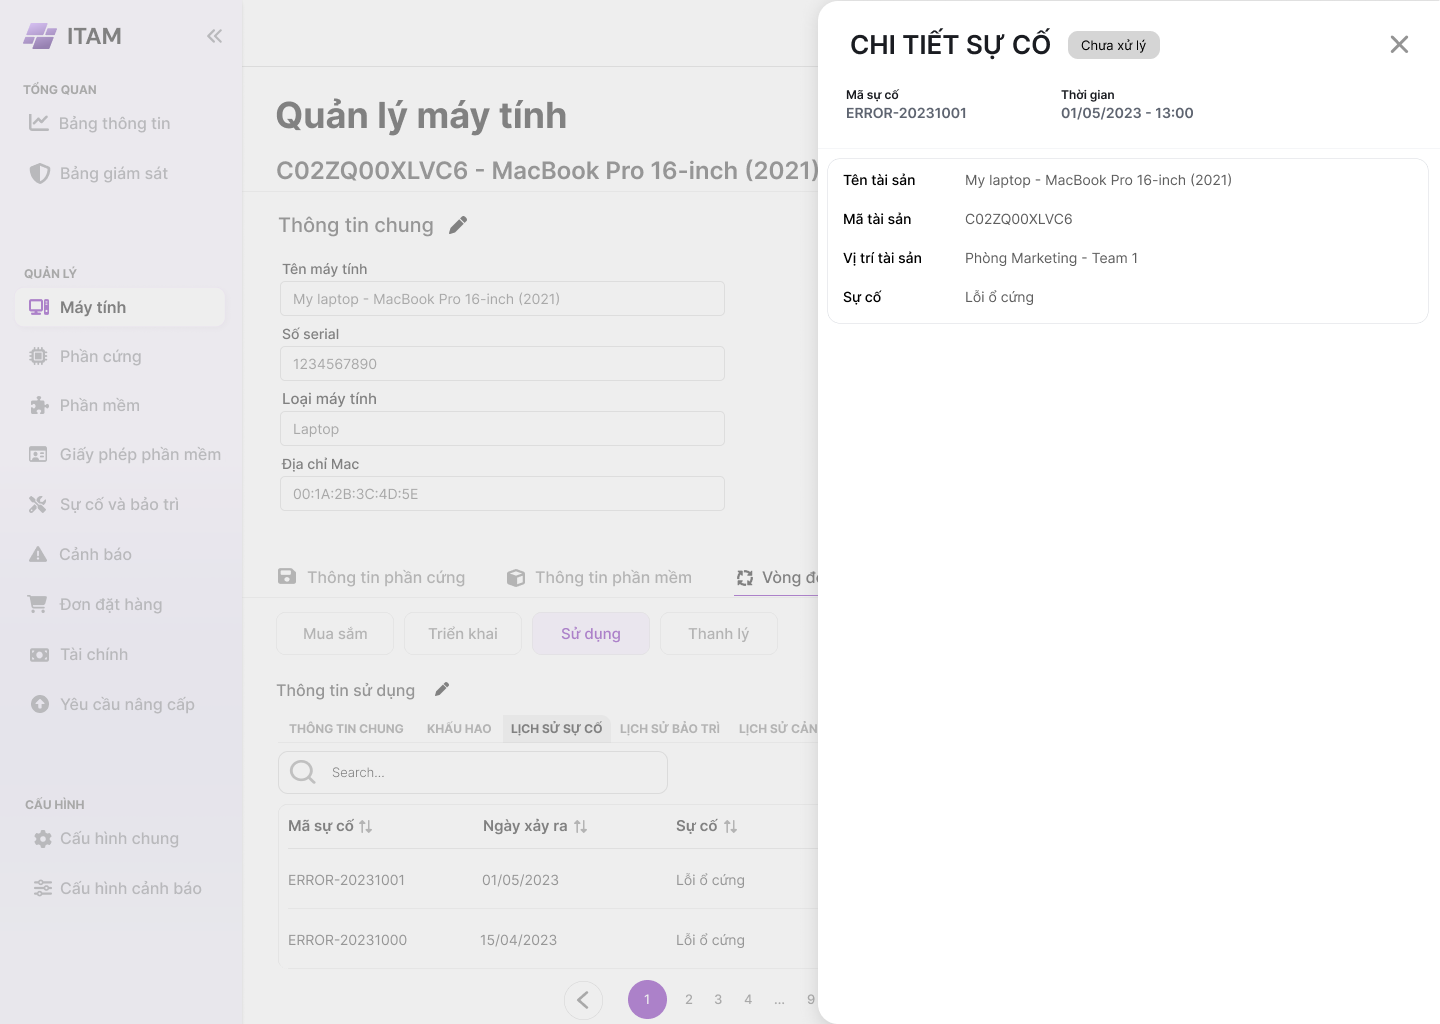
\includegraphics[width=14cm]{Images/C5/UI/Feature-Giám sát tài sản-Máy tính 6.6.png}
%     \vspace{15pt}
%     \caption{Giao diện Quản lý máy tính 15}
% \end{figure}
% \begin{figure}[H]
%     \centering
%     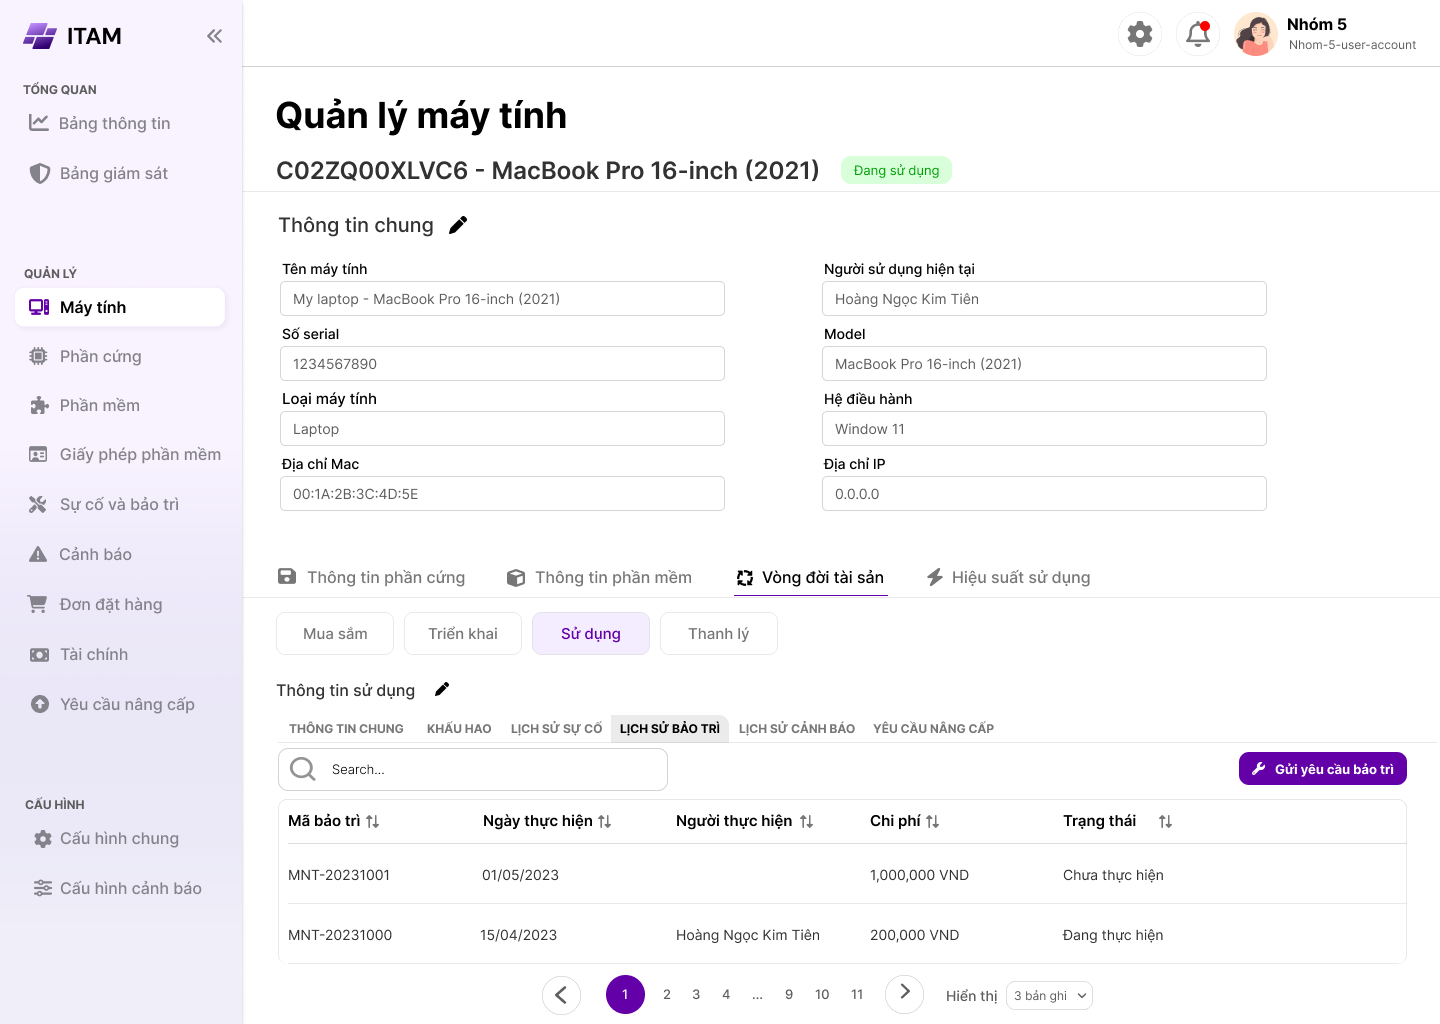
\includegraphics[width=14cm]{Images/C5/UI/Feature-Giám sát tài sản-Máy tính 6.8.png}
%     \vspace{15pt}
%     \caption{Giao diện Quản lý máy tính 10}
% \end{figure}
% \begin{figure}[H]
%     \centering
%     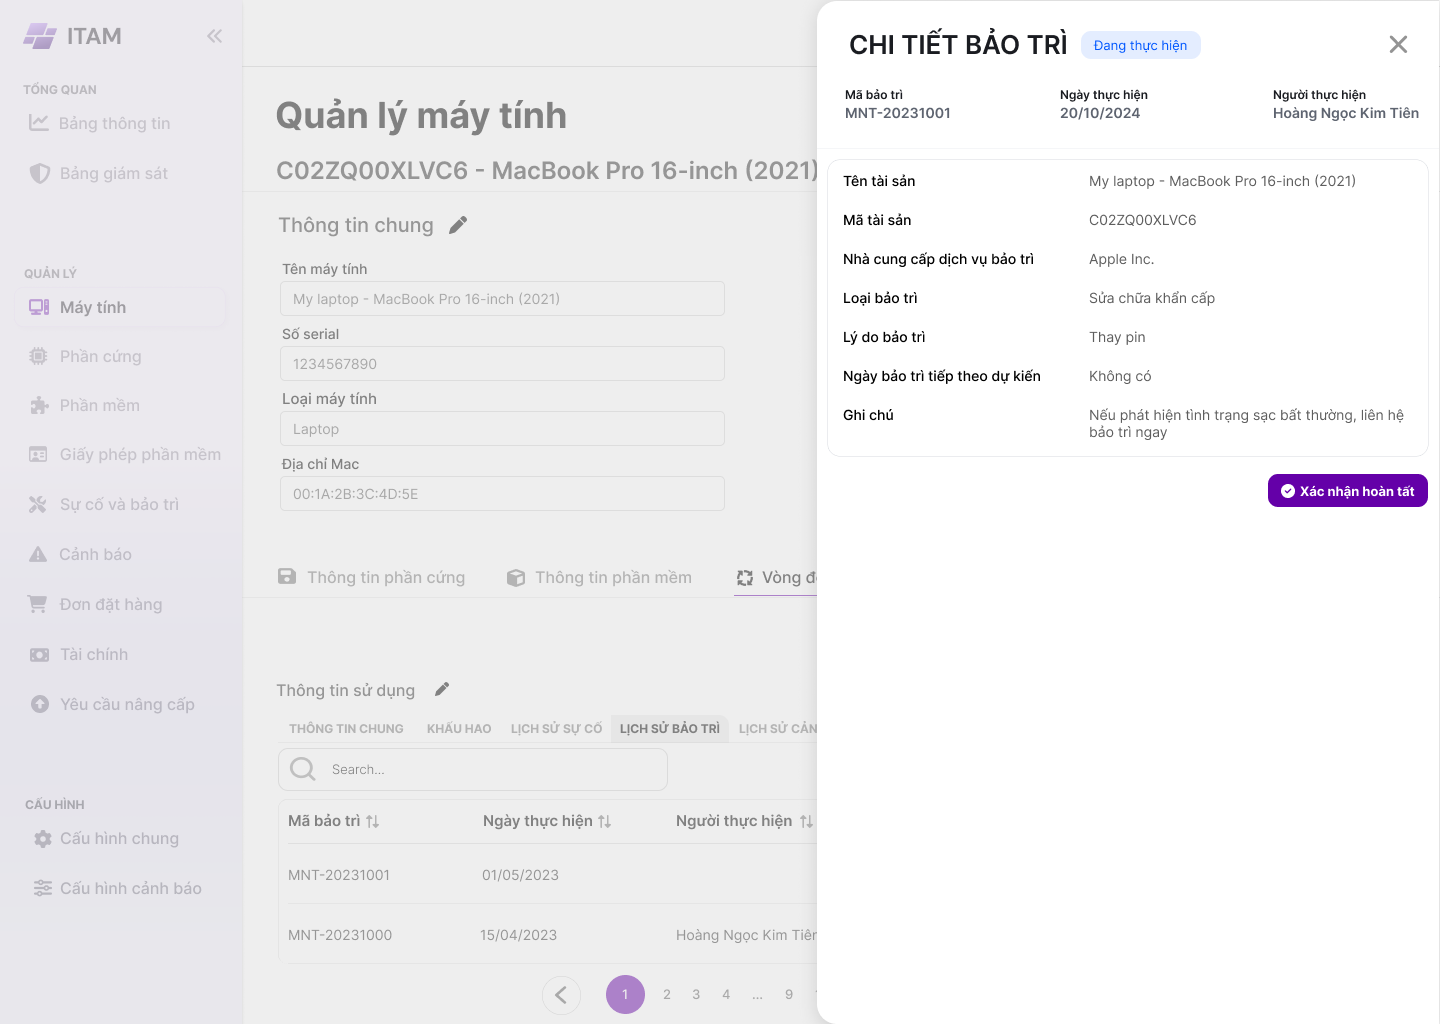
\includegraphics[width=14cm]{Images/C5/UI/Feature-Giám sát tài sản-Máy tính 6.9.png}
%     \vspace{15pt}
%     \caption{Giao diện Quản lý máy tính 17}
% \end{figure}
% \begin{figure}[H]
%     \centering
%     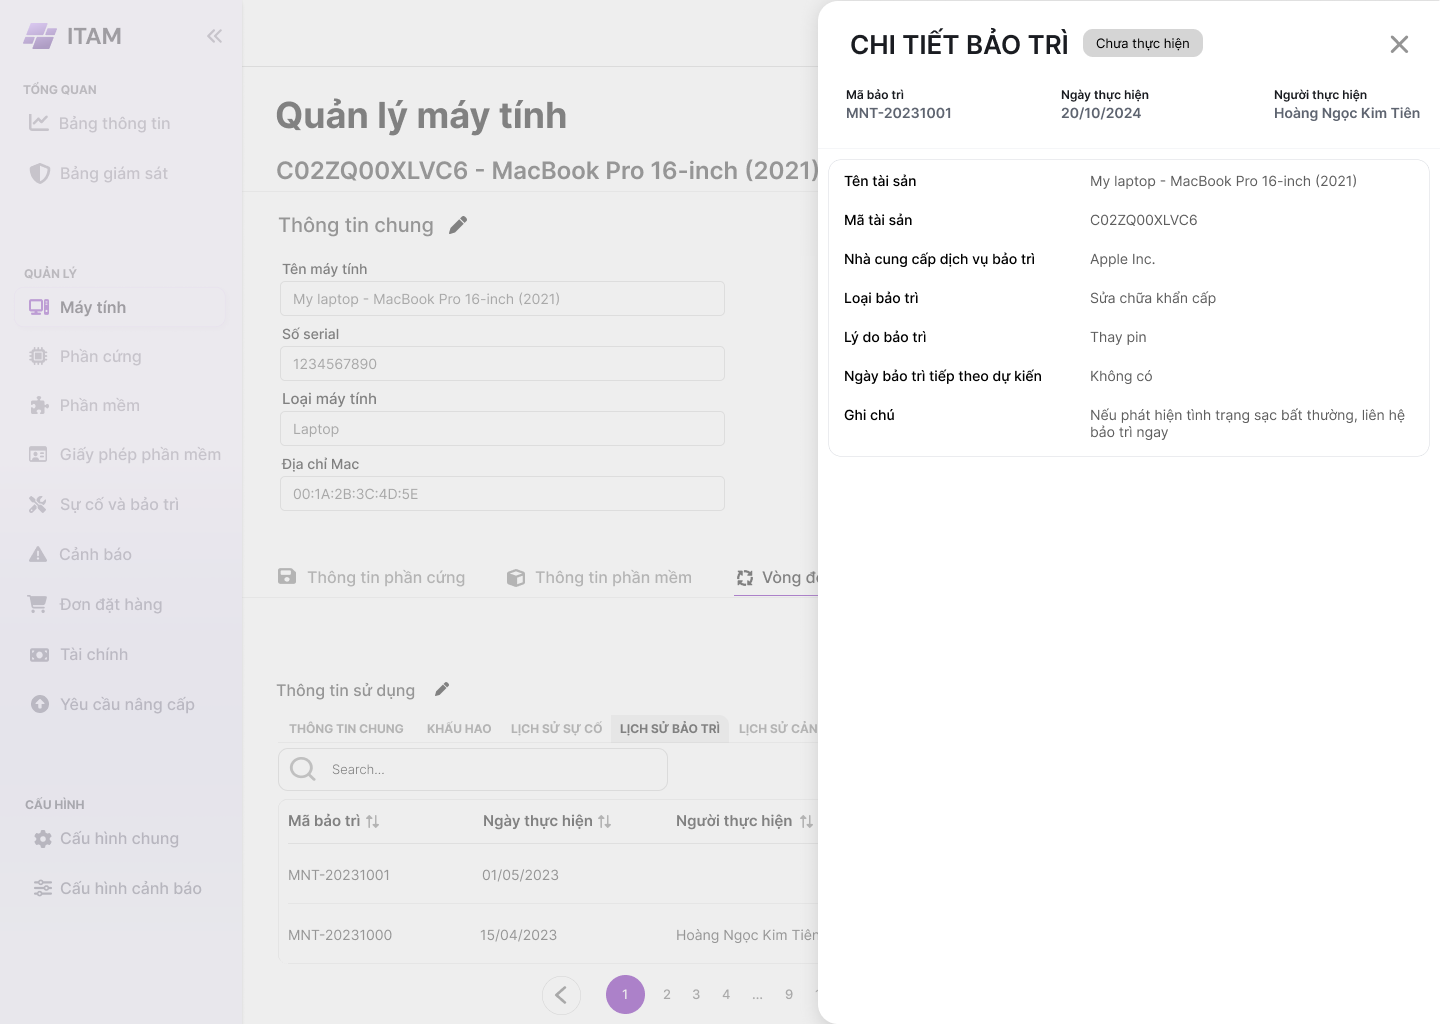
\includegraphics[width=14cm]{Images/C5/UI/Feature-Giám sát tài sản-Máy tính 6.10.png}
%     \vspace{15pt}
%     \caption{Giao diện Quản lý máy tính 18}
% \end{figure}
% \begin{figure}[H]
%     \centering
%     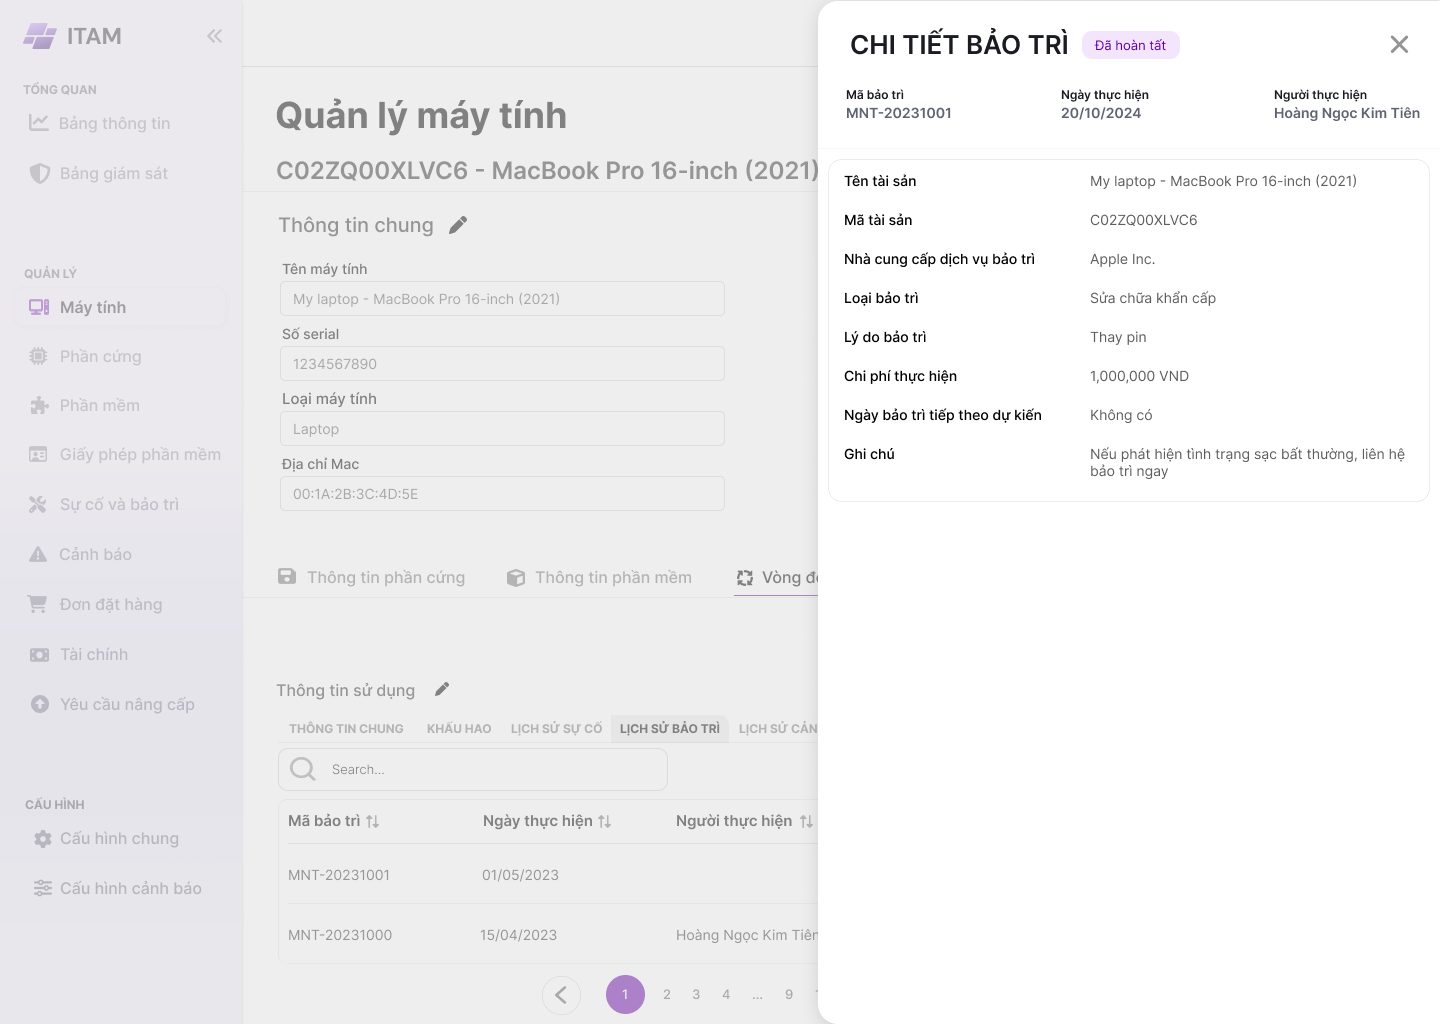
\includegraphics[width=14cm]{Images/C5/UI/Feature-Giám sát tài sản-Máy tính 6.11.png}
%     \vspace{15pt}
%     \caption{Giao diện Quản lý máy tính 19} 
% \end{figure}
% \begin{figure}[H]
%     \centering
%     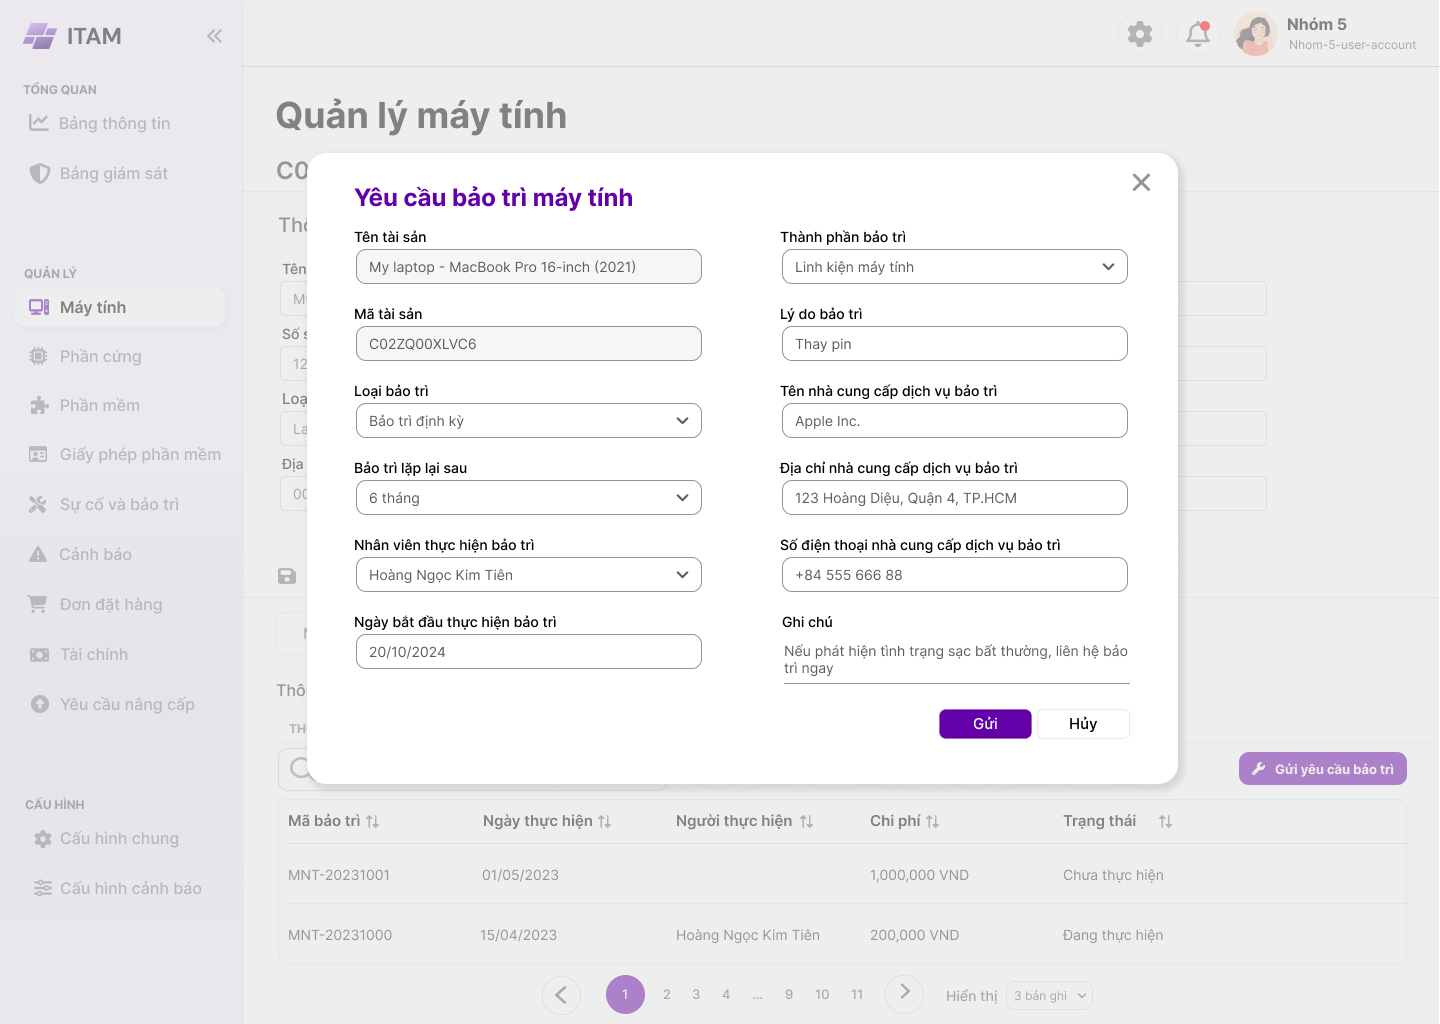
\includegraphics[width=14cm]{Images/C5/UI/Feature-Giám sát tài sản-Máy tính 6.12.png}
%     \vspace{15pt}
%     \caption{Giao diện Quản lý máy tính 11}
% \end{figure}
% \begin{figure}[H]
%     \centering
%     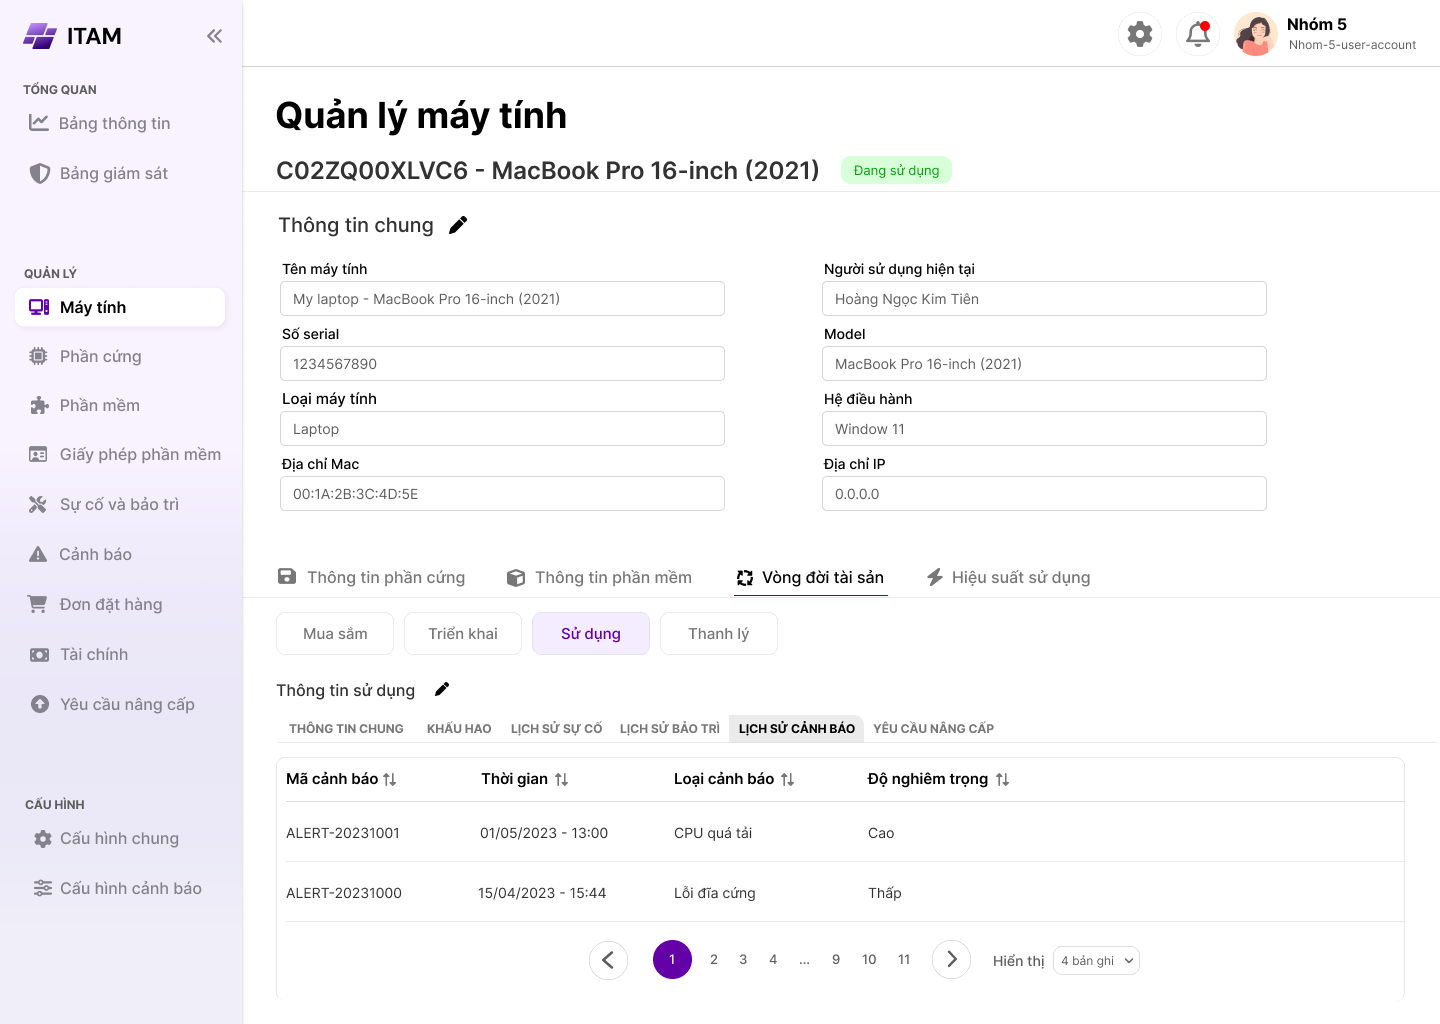
\includegraphics[width=14cm]{Images/C5/UI/Feature-Giám sát tài sản-Máy tính 6.13.png}
%     \vspace{15pt}
%     \caption{Giao diện Quản lý máy tính 15}
% \end{figure}
% \begin{figure}[H]
%     \centering
%     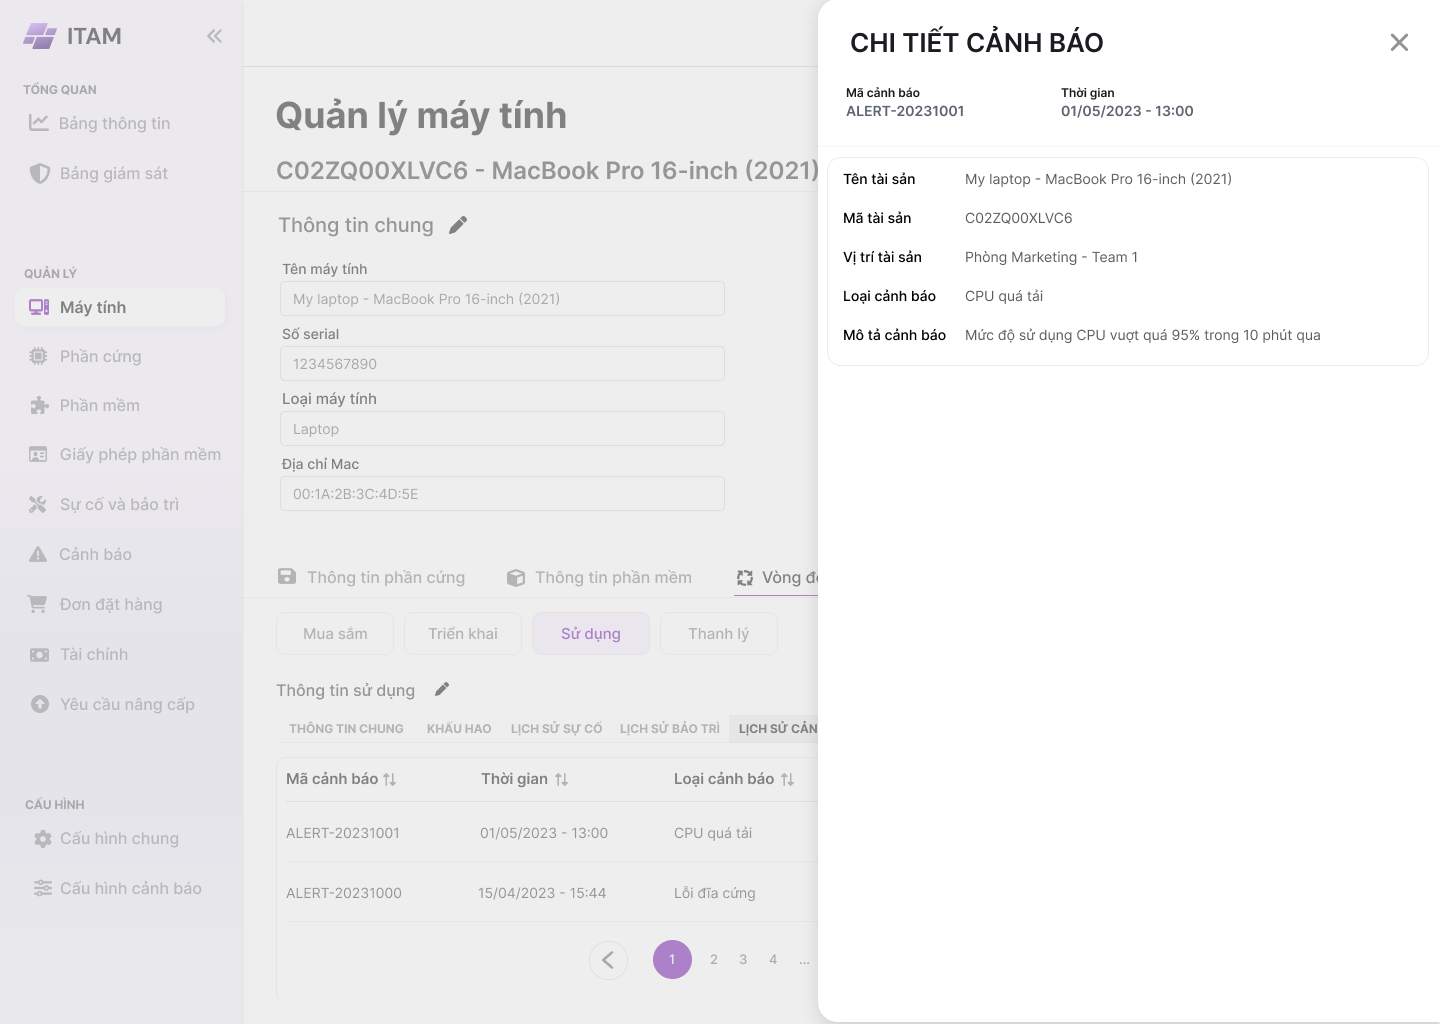
\includegraphics[width=14cm]{Images/C5/UI/Feature-Giám sát tài sản-Máy tính 6.14.png}
%     \vspace{15pt}
%     \caption{Giao diện Quản lý máy tính 22}
% \end{figure}
% \begin{figure}[H]
%     \centering
%     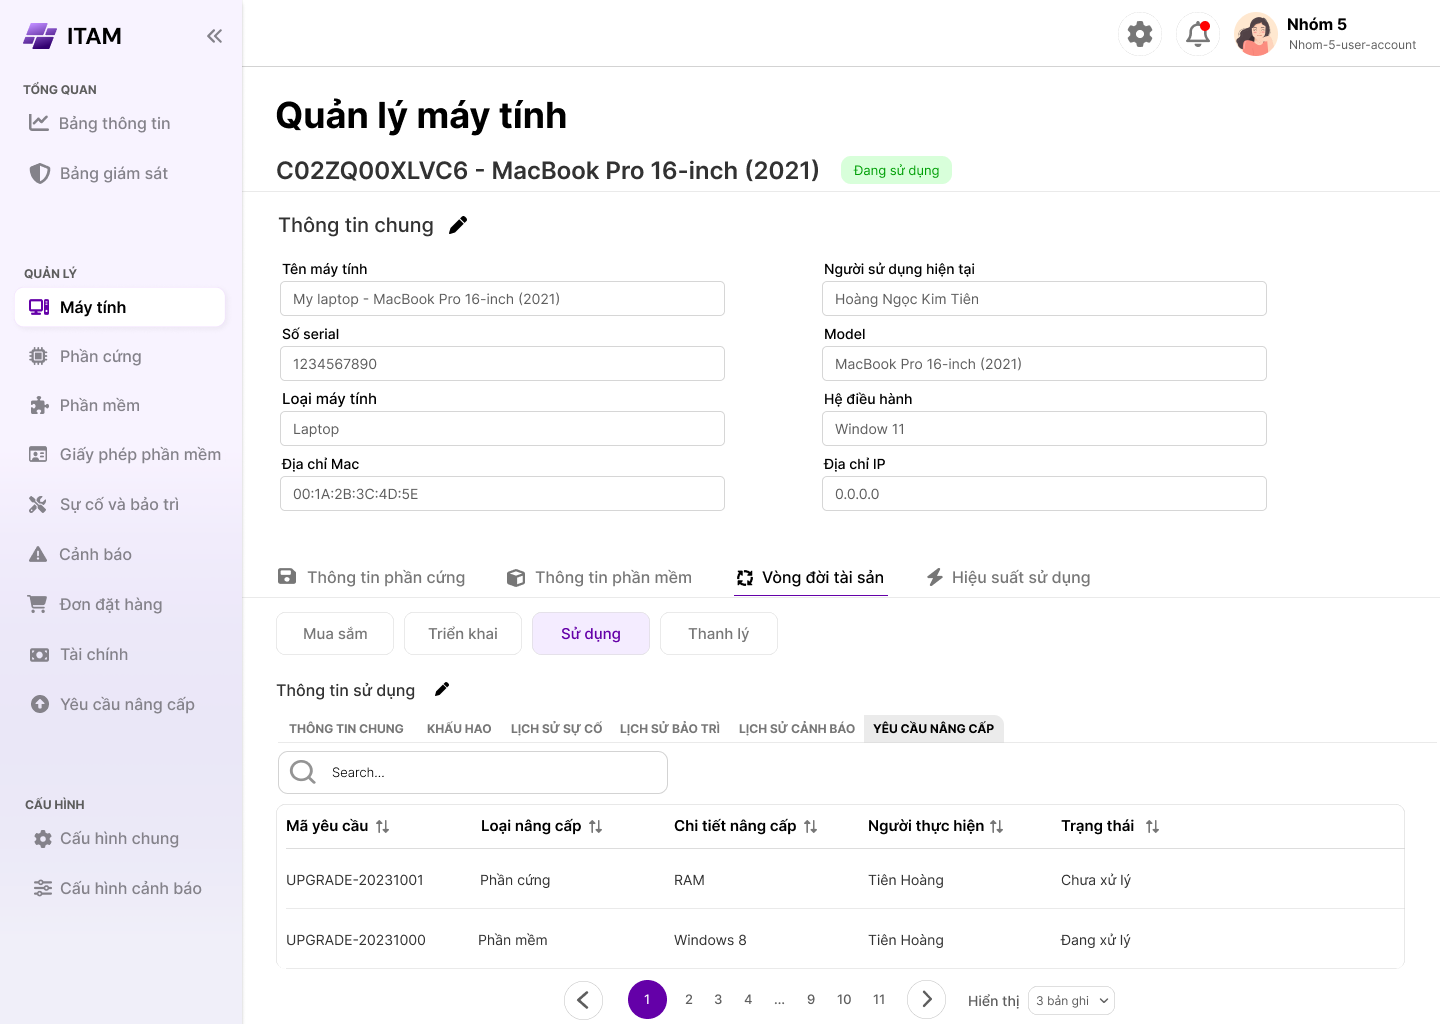
\includegraphics[width=14cm]{Images/C5/UI/Feature-Giám sát tài sản-Máy tính 6.15.png}
%     \vspace{15pt}
%     \caption{Giao diện Quản lý máy tính 16}
% \end{figure}
% \begin{figure}[H]
%     \centering
%     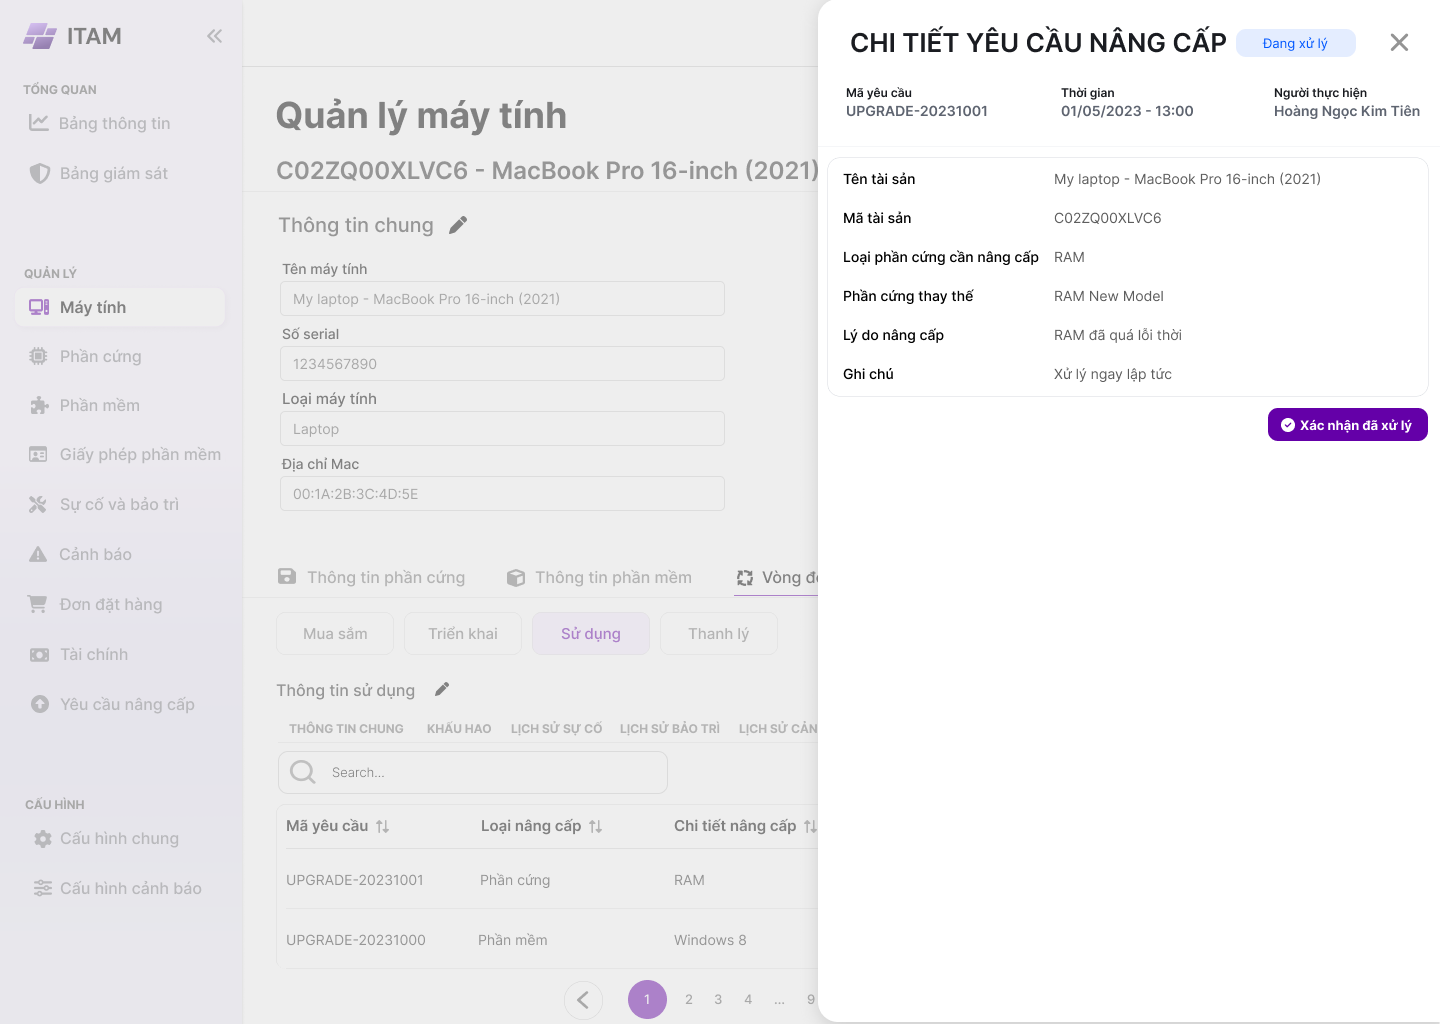
\includegraphics[width=14cm]{Images/C5/UI/Feature-Giám sát tài sản-Máy tính 6.16.png}
%     \vspace{15pt}
%     \caption{Giao diện Quản lý máy tính 24}
% \end{figure}
% \begin{figure}[H]
%     \centering
%     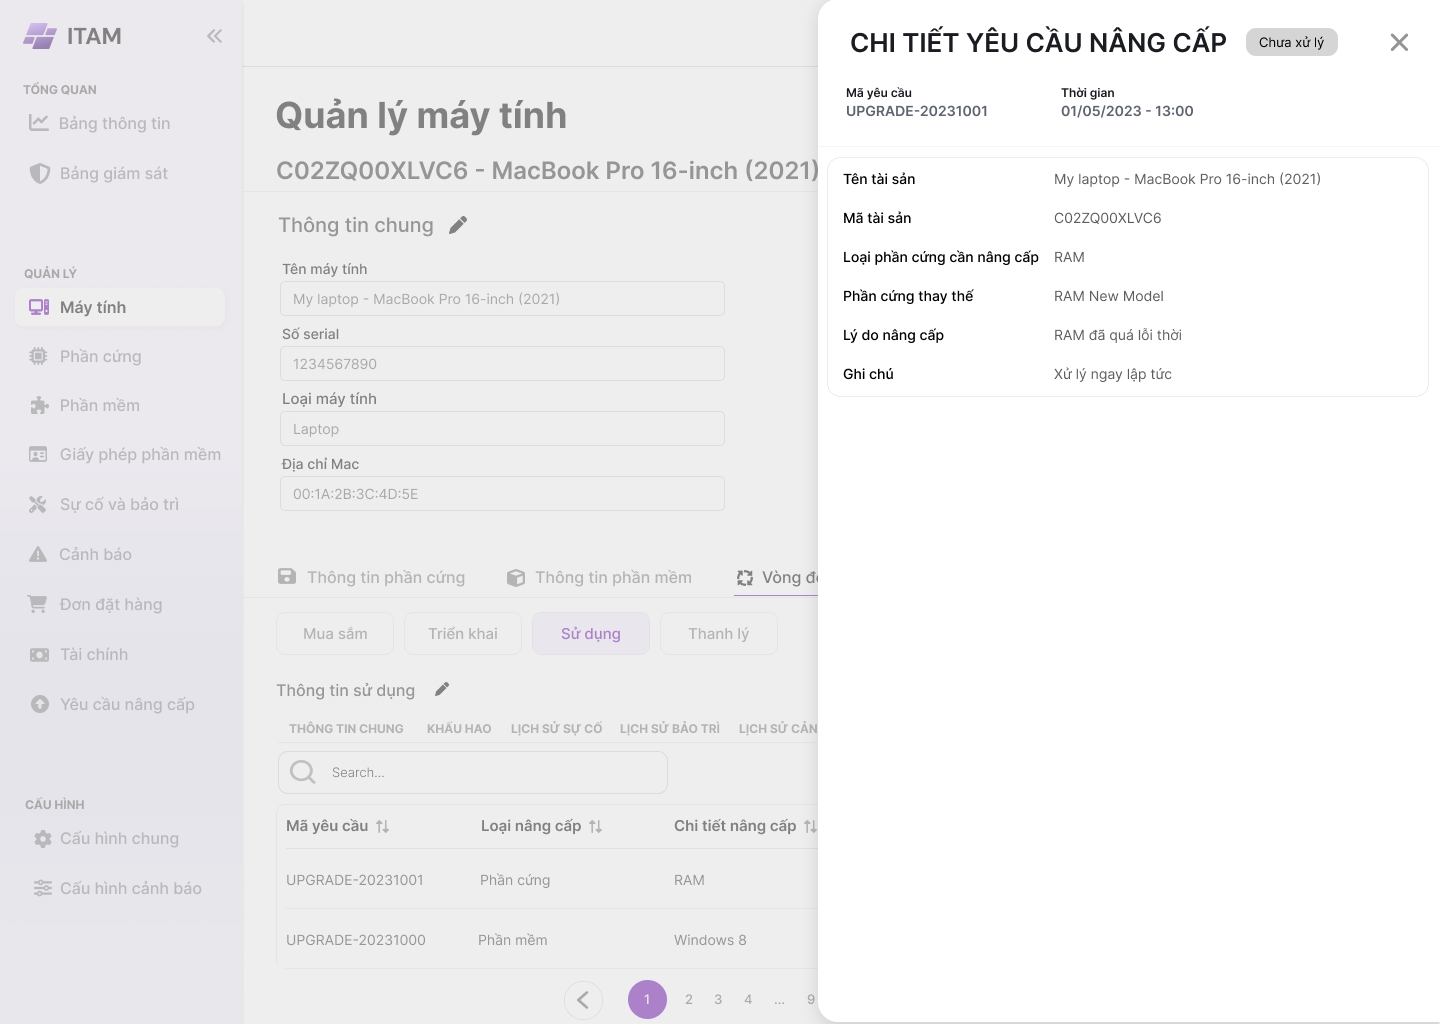
\includegraphics[width=14cm]{Images/C5/UI/Feature-Giám sát tài sản-Máy tính 6.17.png}
%     \vspace{15pt}
%     \caption{Giao diện Quản lý máy tính 25}
% \end{figure}
% \begin{figure}[H]
%     \centering
%     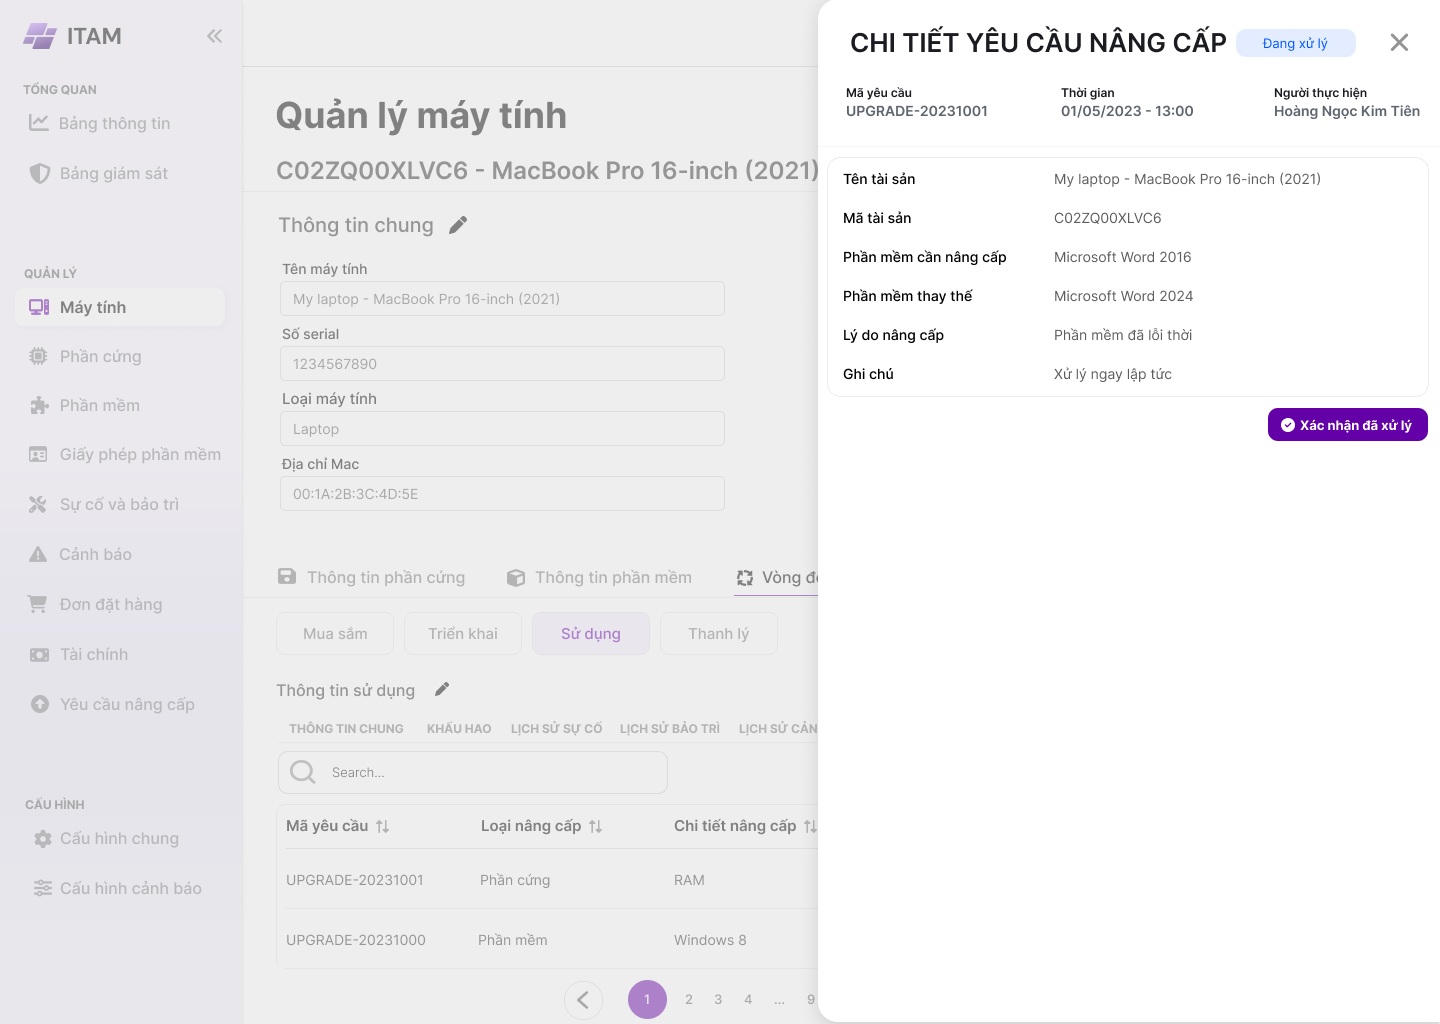
\includegraphics[width=14cm]{Images/C5/UI/Feature-Giám sát tài sản-Máy tính 6.18.png}
%     \vspace{15pt}
%     \caption{Giao diện Quản lý máy tính 26}
% \end{figure}
% \begin{figure}[H]
%     \centering
%     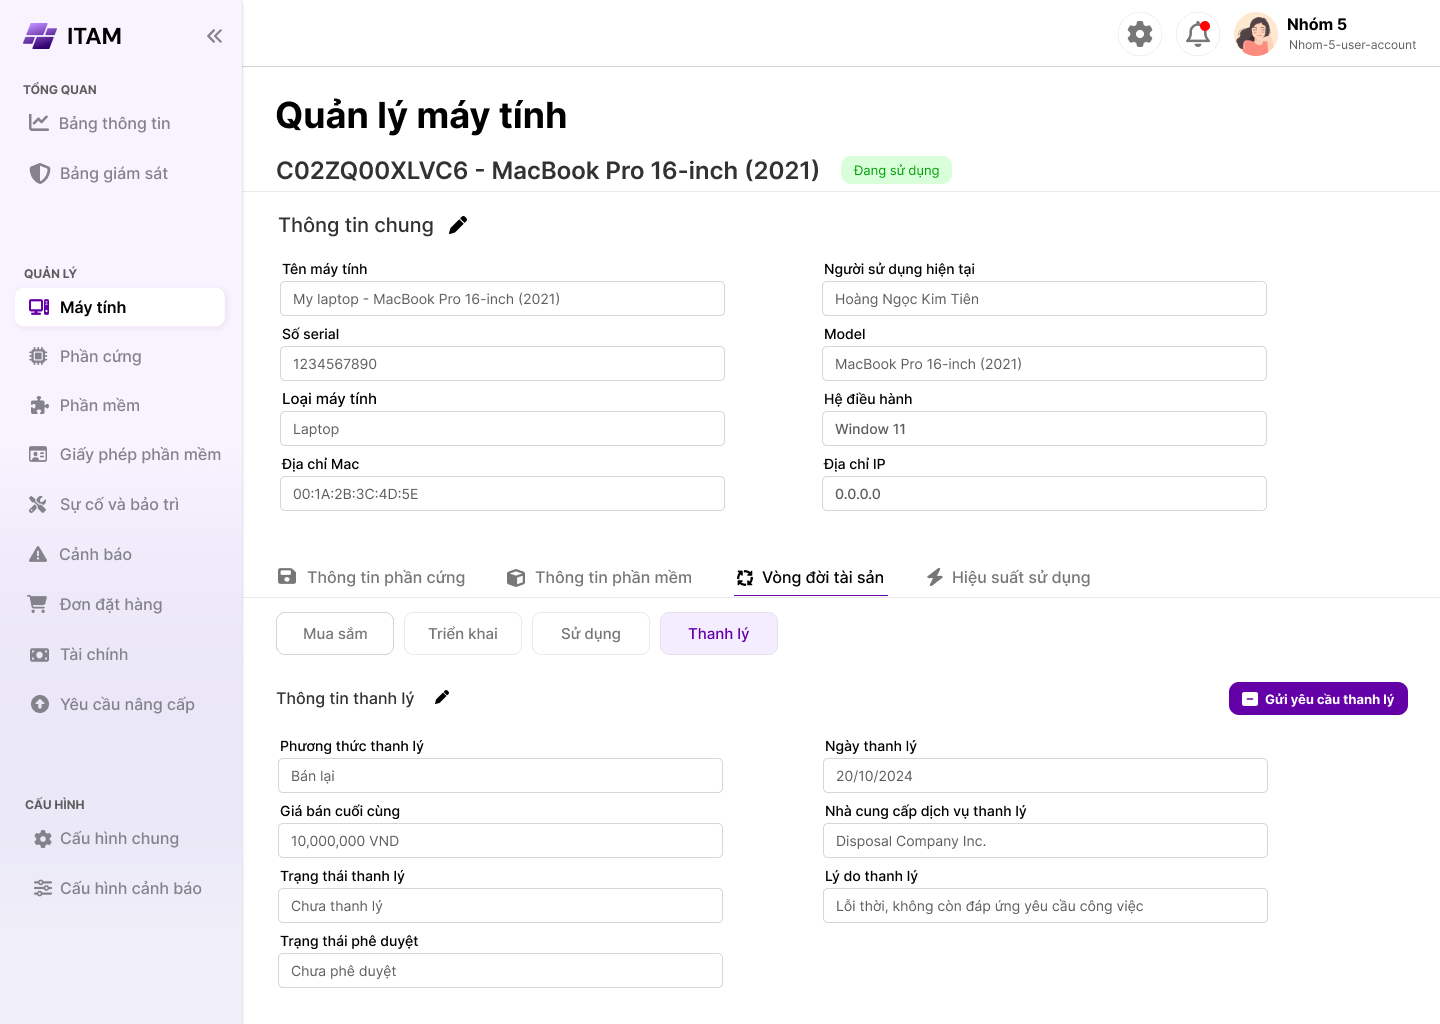
\includegraphics[width=14cm]{Images/C5/UI/Feature-Giám sát tài sản-Máy tính 7.1.png}
%     \vspace{15pt}
%     \caption{Giao diện Quản lý máy tính 12}
% \end{figure}
% \begin{figure}[H]
%     \centering
%     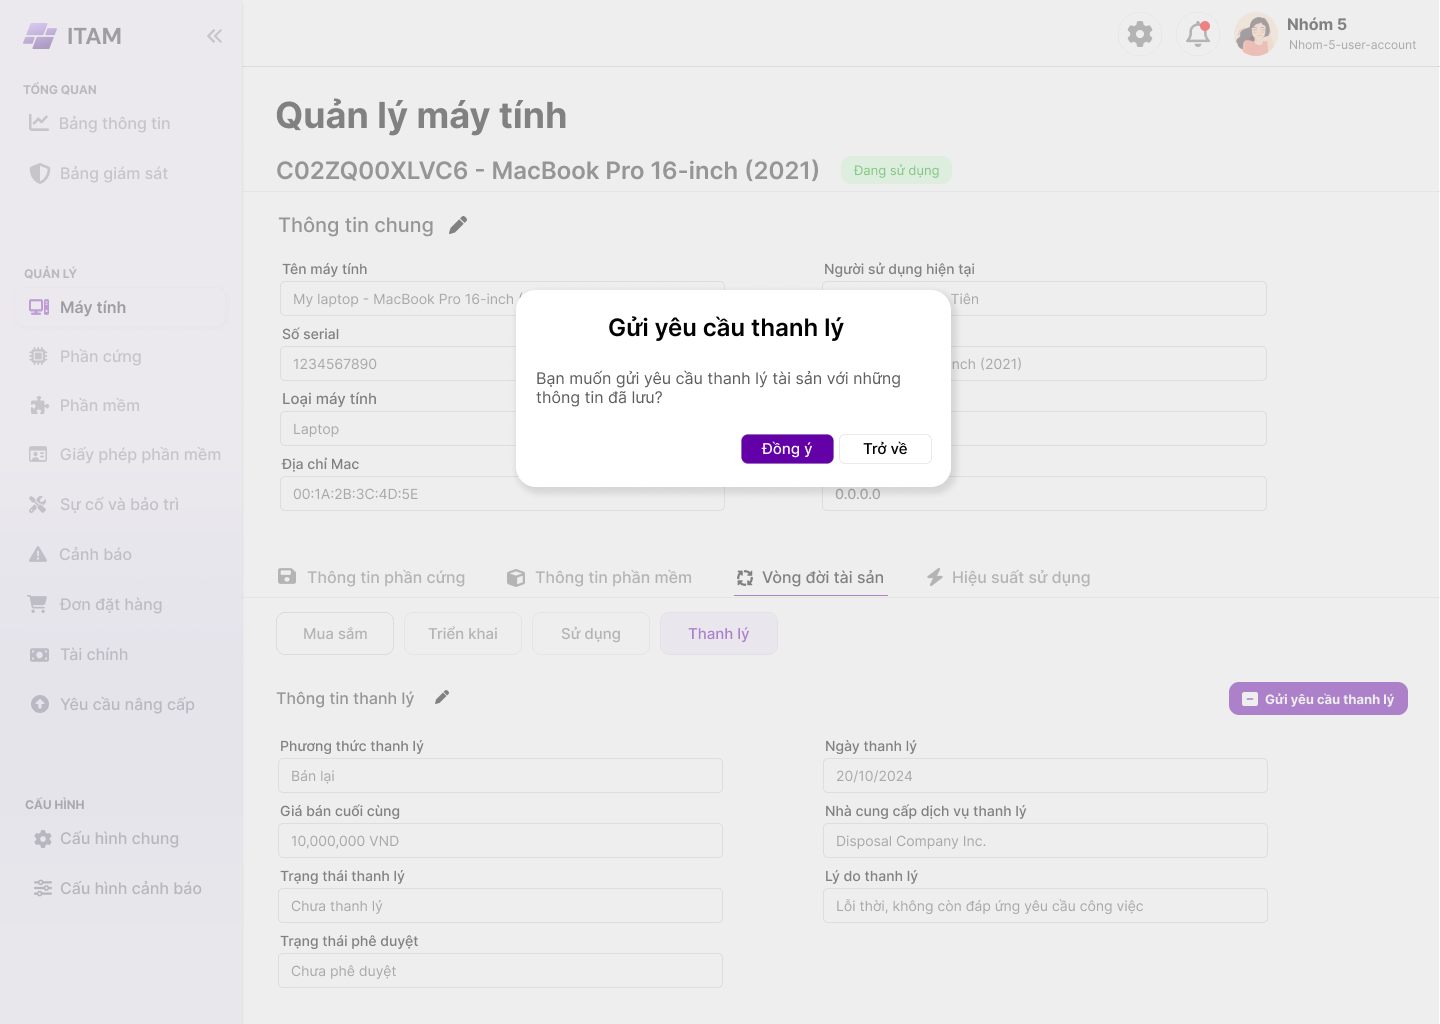
\includegraphics[width=14cm]{Images/C5/UI/Feature-Giám sát tài sản-Máy tính 7.2.png}
%     \vspace{15pt}
%     \caption{Giao diện Quản lý máy tính 28}
% \end{figure}
% \begin{figure}[H]
%     \centering
%     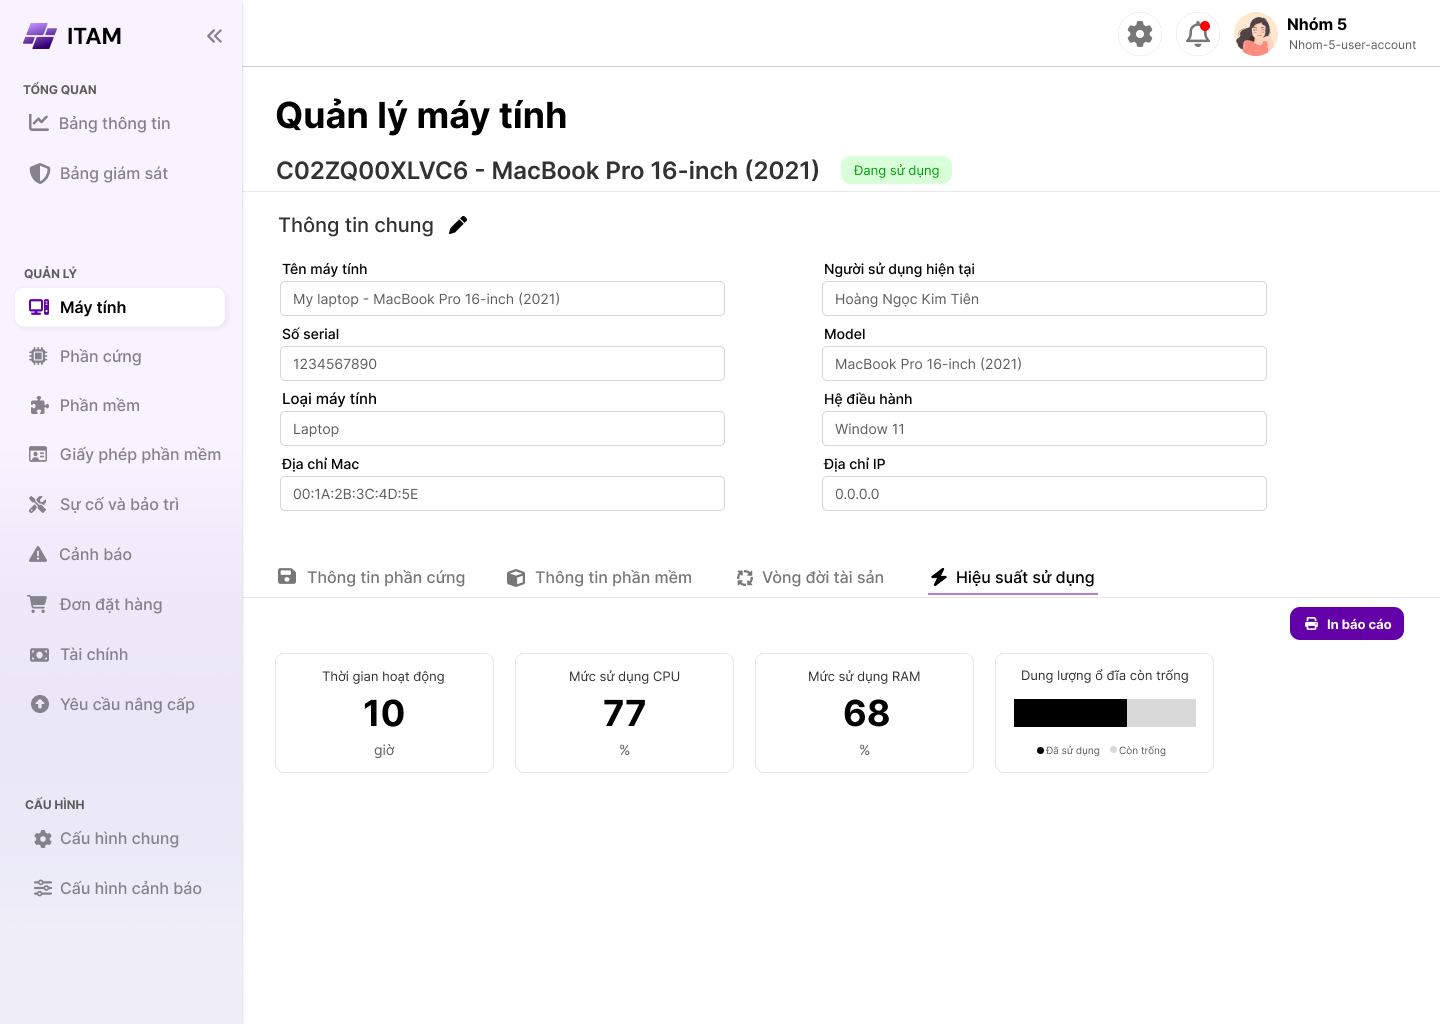
\includegraphics[width=14cm]{Images/C5/UI/Feature-Giám sát tài sản-Máy tính 9.1.png}
%     \vspace{15pt}
%     \caption{Giao diện Quản lý máy tính 2}
% \end{figure}
\begin{figure}[H]
    \centering
    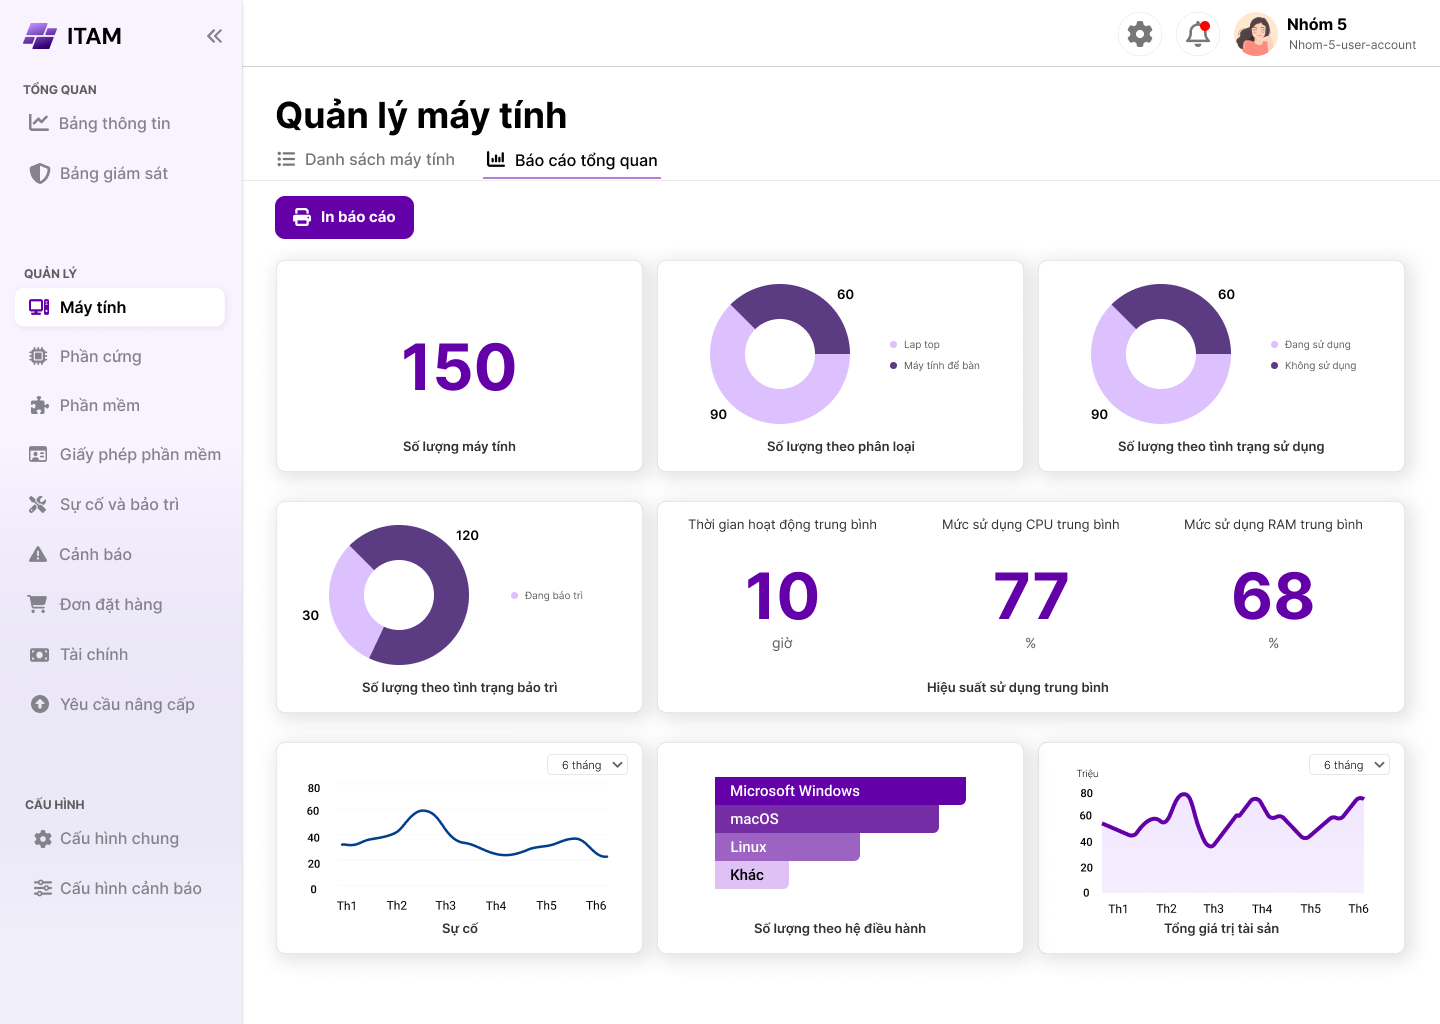
\includegraphics[width=14cm]{Images/C5/UI/Feature-Giám sát tài sản-Máy tính 10.png}
    \vspace{15pt}
    \caption{Giao diện Quản lý máy tính 2}
\end{figure}

\item{Quản lý phần cứng}\\
Ở chức năng Quản lý phần cứng, người dùng có thể dễ dàng xem danh sách tất cả các phần cứng trong hệ thống, thêm mới phần cứng, xem chi tiết phần cứng, gửi yêu cầu bảo trì cho phần cứng, và xem báo cáo tổng quan về phần cứng (xem thêm chi tiết ở phụ lục).
% \begin{figure}[H]
%     \centering
%     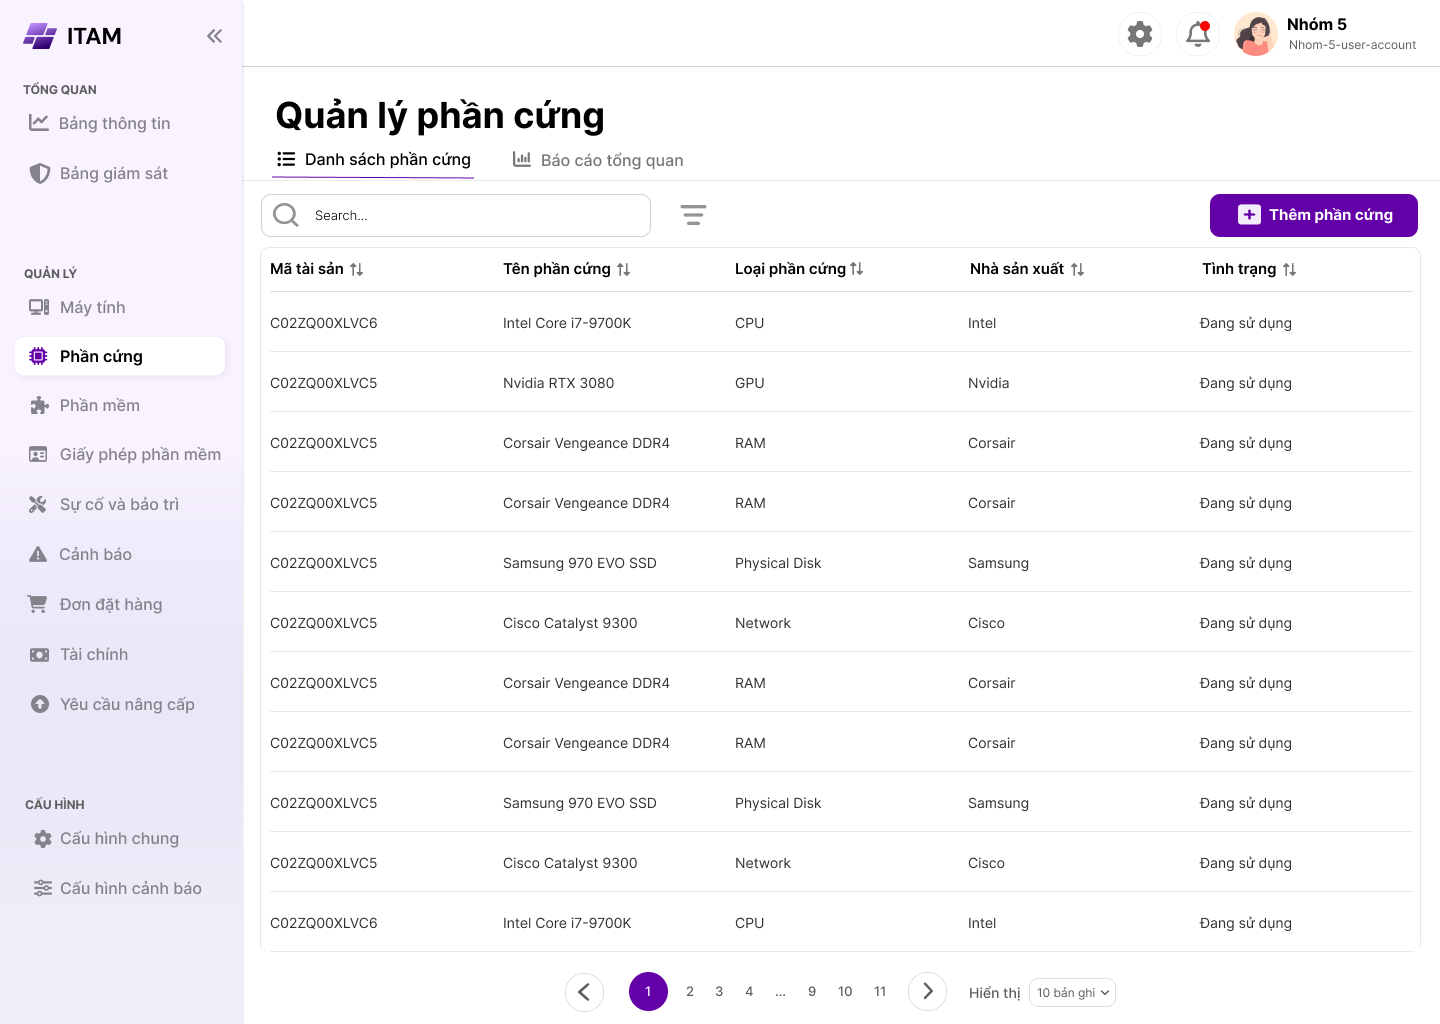
\includegraphics[width=14cm]{Images/C5/UI/Feature-Giám sát tài sản-Phần cứng 1.png}
%     \vspace{15pt}
%     \caption{Giao diện Quản lý phần cứng 1}
% \end{figure}
% \begin{figure}[H]
%     \centering
%     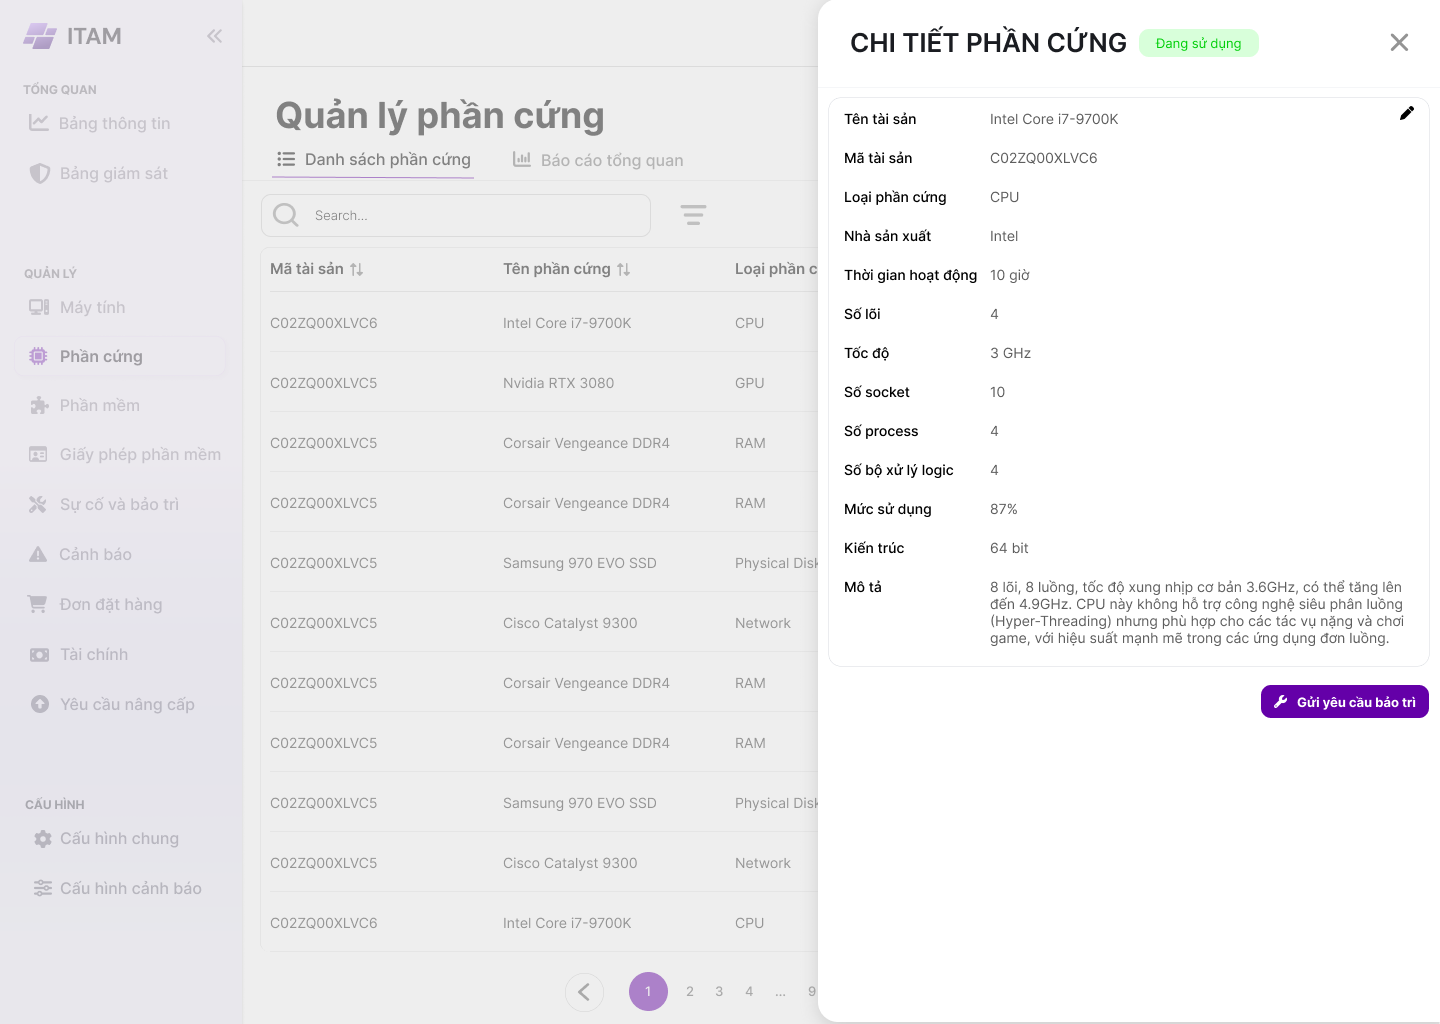
\includegraphics[width=14cm]{Images/C5/UI/Feature-Giám sát tài sản-Phần cứng 2.1-CPU.png}
%     \vspace{15pt}
%     \caption{Giao diện Quản lý phần cứng 2}
% \end{figure}
% \begin{figure}[H]
%     \centering
%     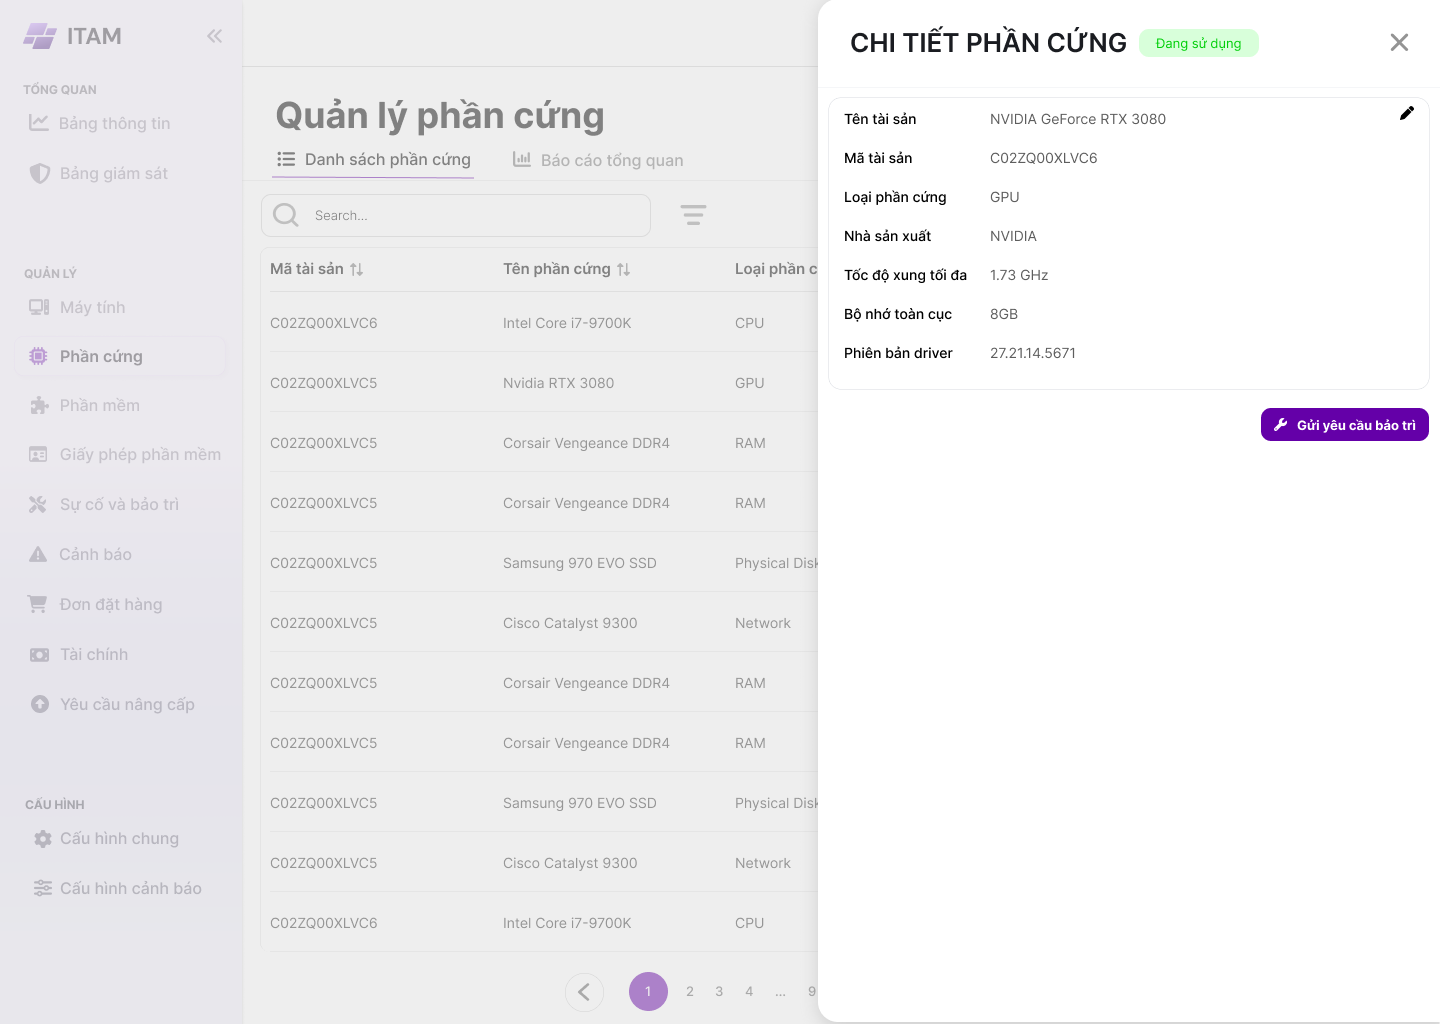
\includegraphics[width=14cm]{Images/C5/UI/Feature-Giám sát tài sản-Phần cứng 2.2-GPU.png}
%     \vspace{15pt}
%     \caption{Giao diện Quản lý phần cứng 3}
% \end{figure}
% \begin{figure}[H]
%     \centering
%     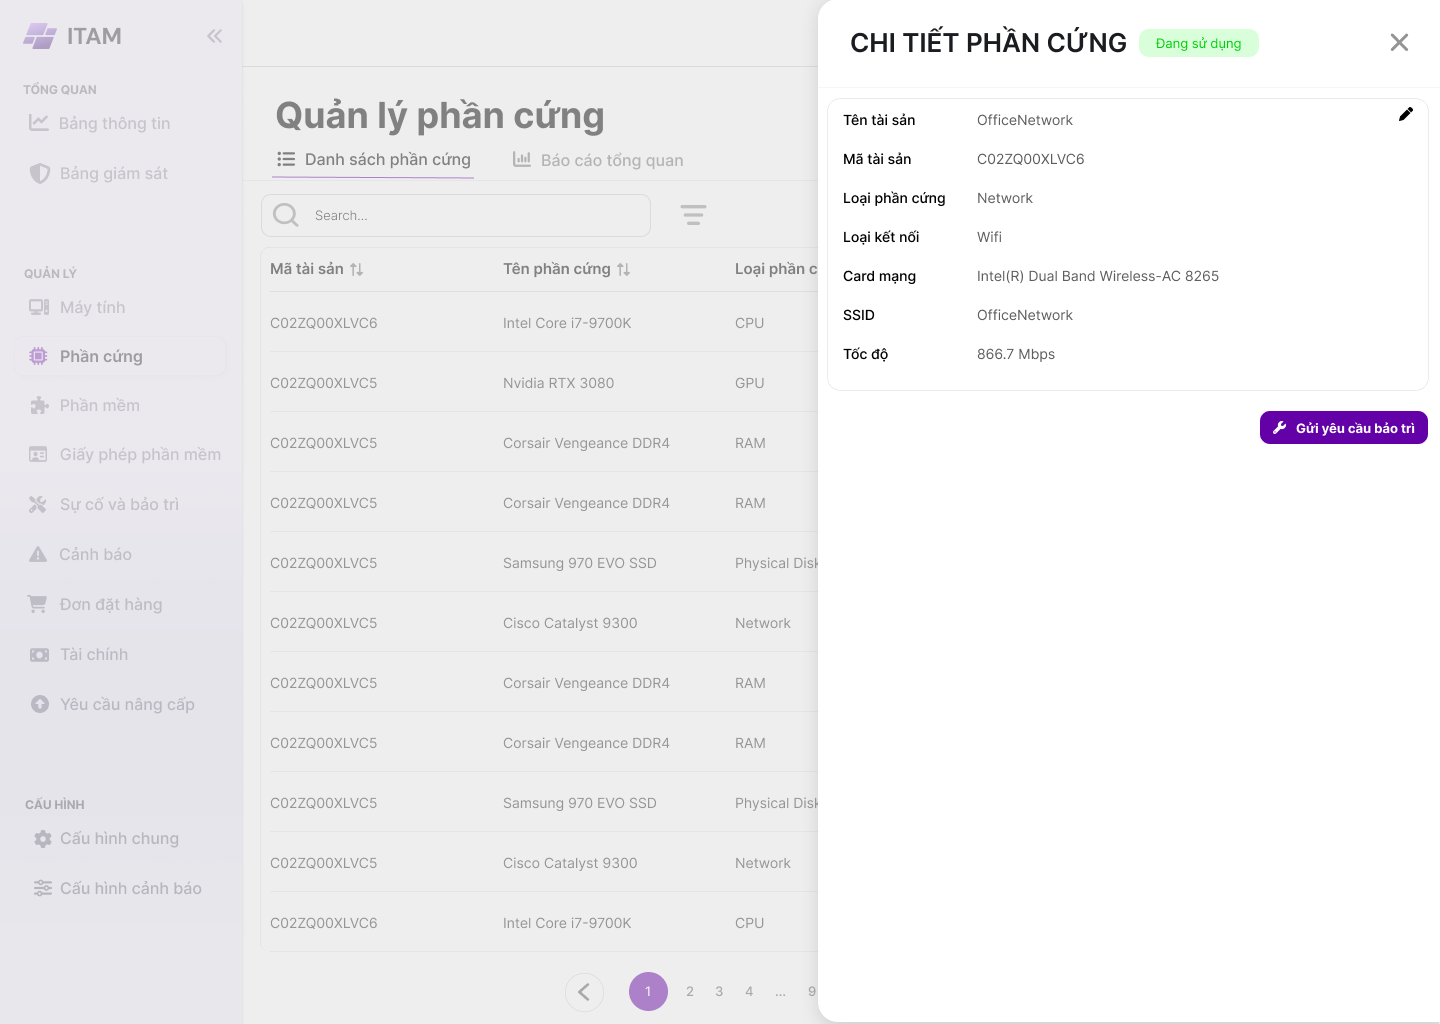
\includegraphics[width=14cm]{Images/C5/UI/Feature-Giám sát tài sản-Phần cứng 2.3-Network.png}
%     \vspace{15pt}
%     \caption{Giao diện Quản lý phần cứng 4}
% \end{figure}
% \begin{figure}[H]
%     \centering
%     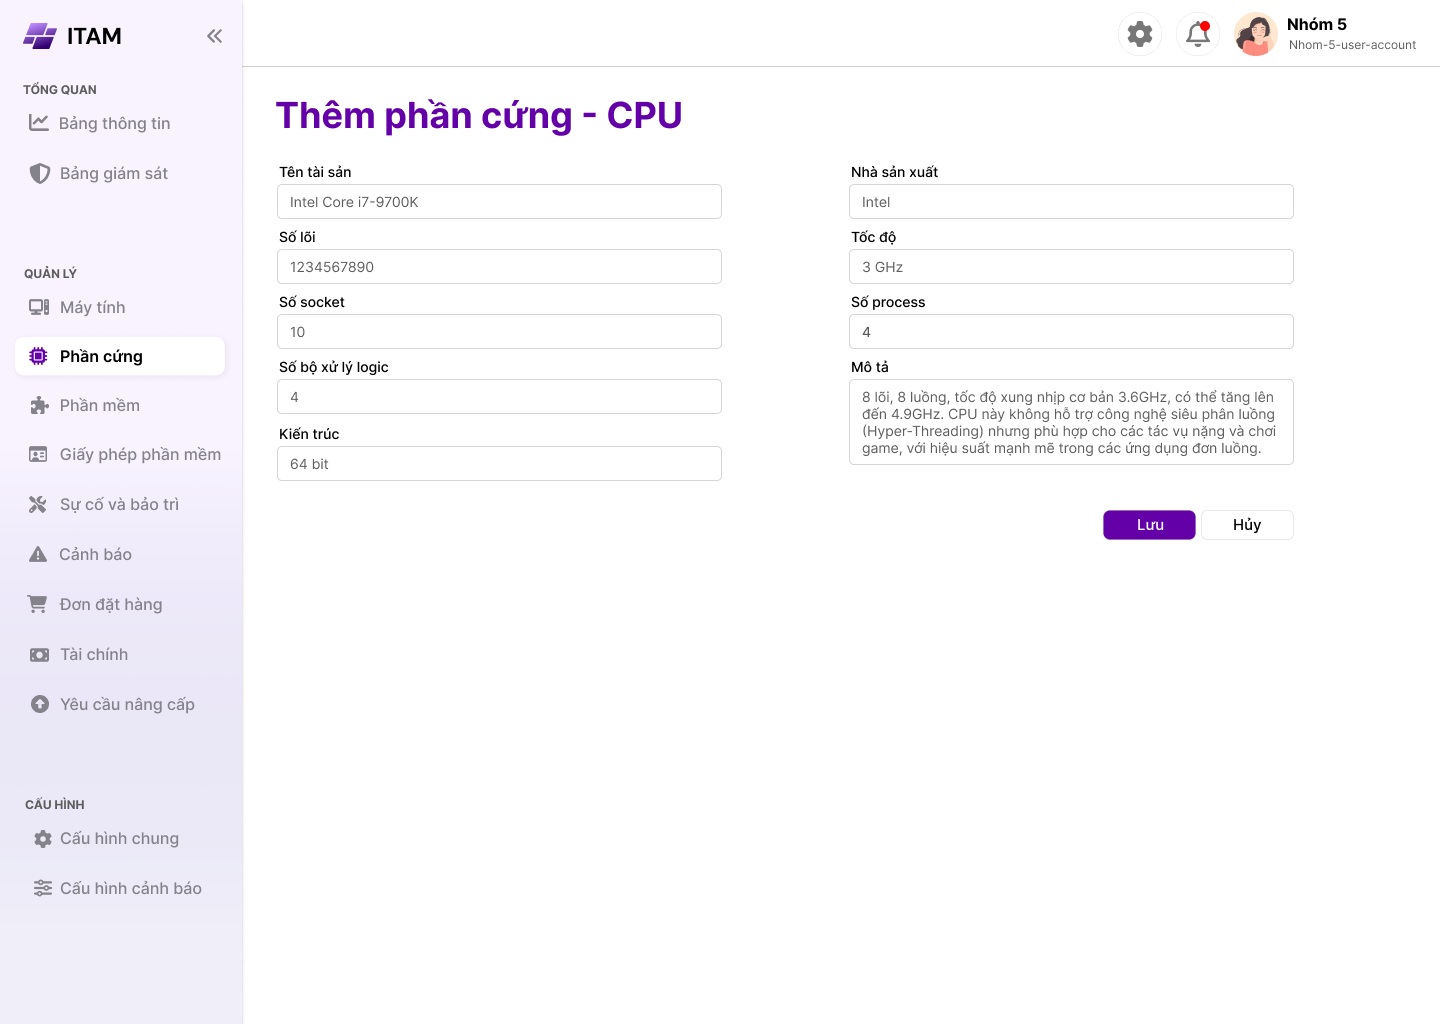
\includegraphics[width=14cm]{Images/C5/UI/Feature-Giám sát tài sản-Phần cứng 4.2.png}
%     \vspace{15pt}
%     \caption{Giao diện Quản lý phần cứng 3}
% \end{figure}
% \begin{figure}[H]
%     \centering
%     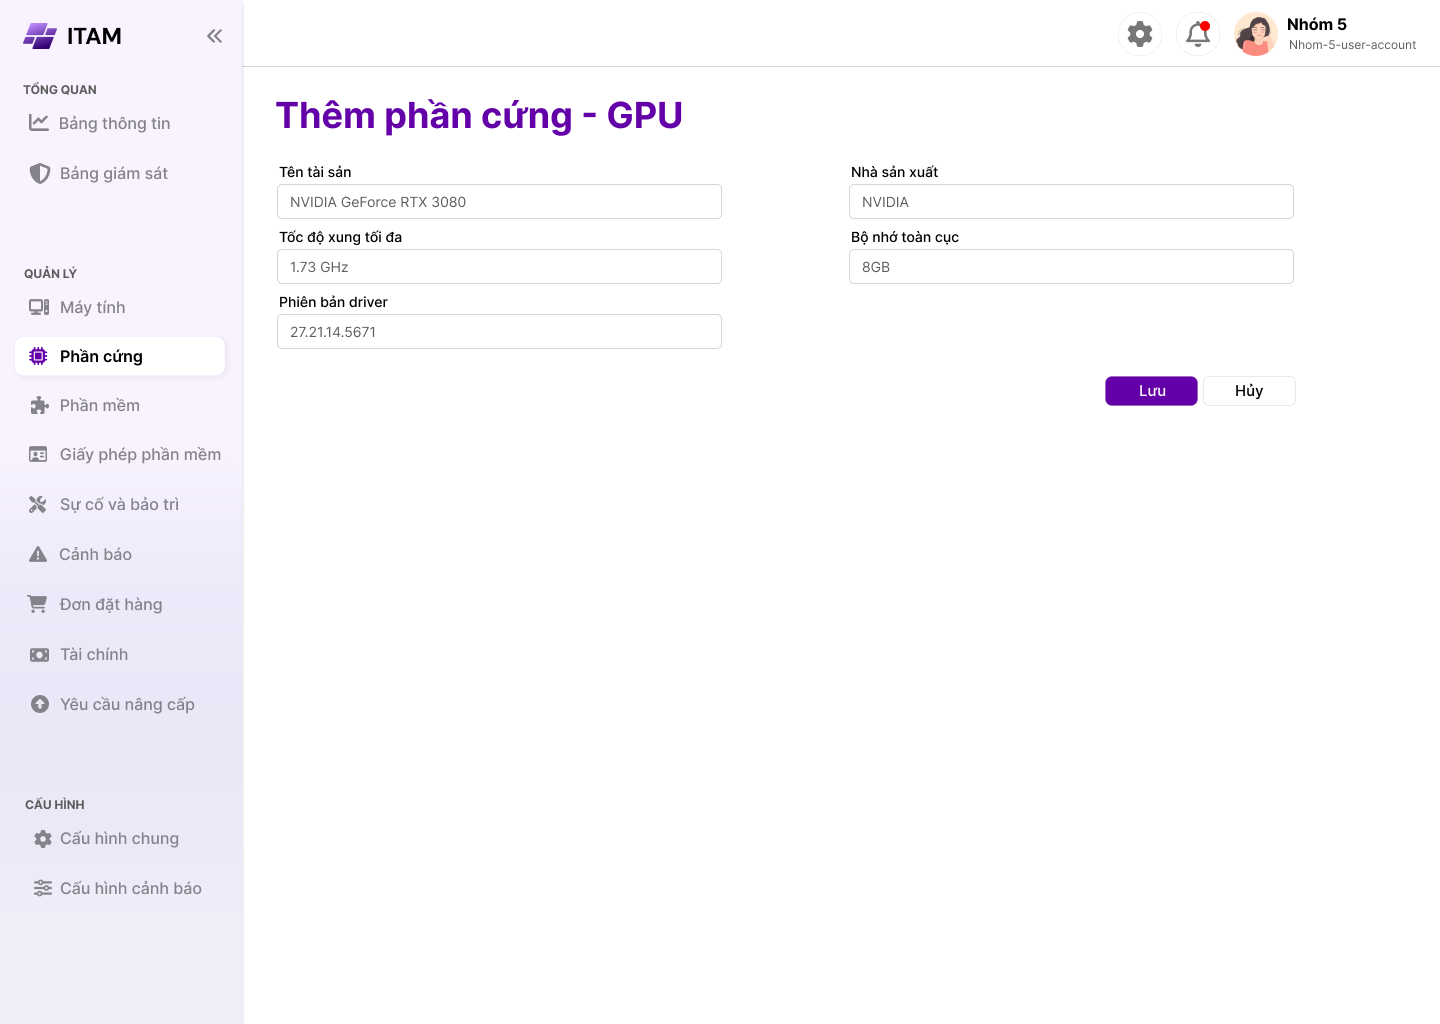
\includegraphics[width=14cm]{Images/C5/UI/Feature-Giám sát tài sản-Phần cứng 4.3.png}
%     \vspace{15pt}
%     \caption{Giao diện Quản lý phần cứng 6}
% \end{figure}
% \begin{figure}[H]
%     \centering
%     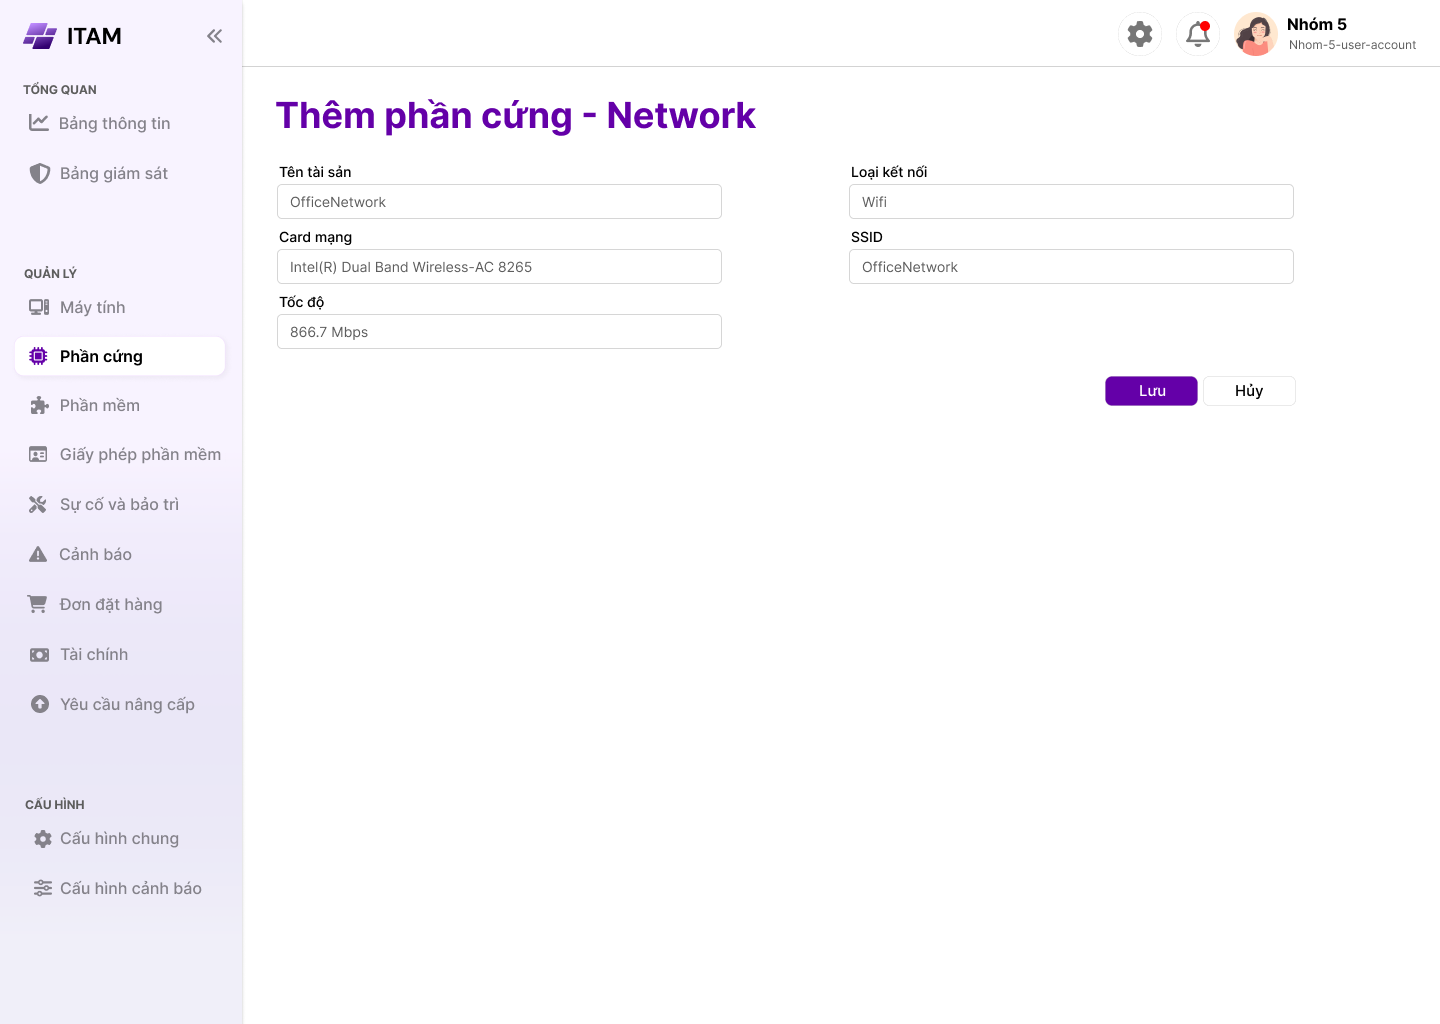
\includegraphics[width=14cm]{Images/C5/UI/Feature-Giám sát tài sản-Phần cứng 4.4.png}
%     \vspace{15pt}
%     \caption{Giao diện Quản lý phần cứng 7}
% \end{figure}
% \begin{figure}[H]
%     \centering
%     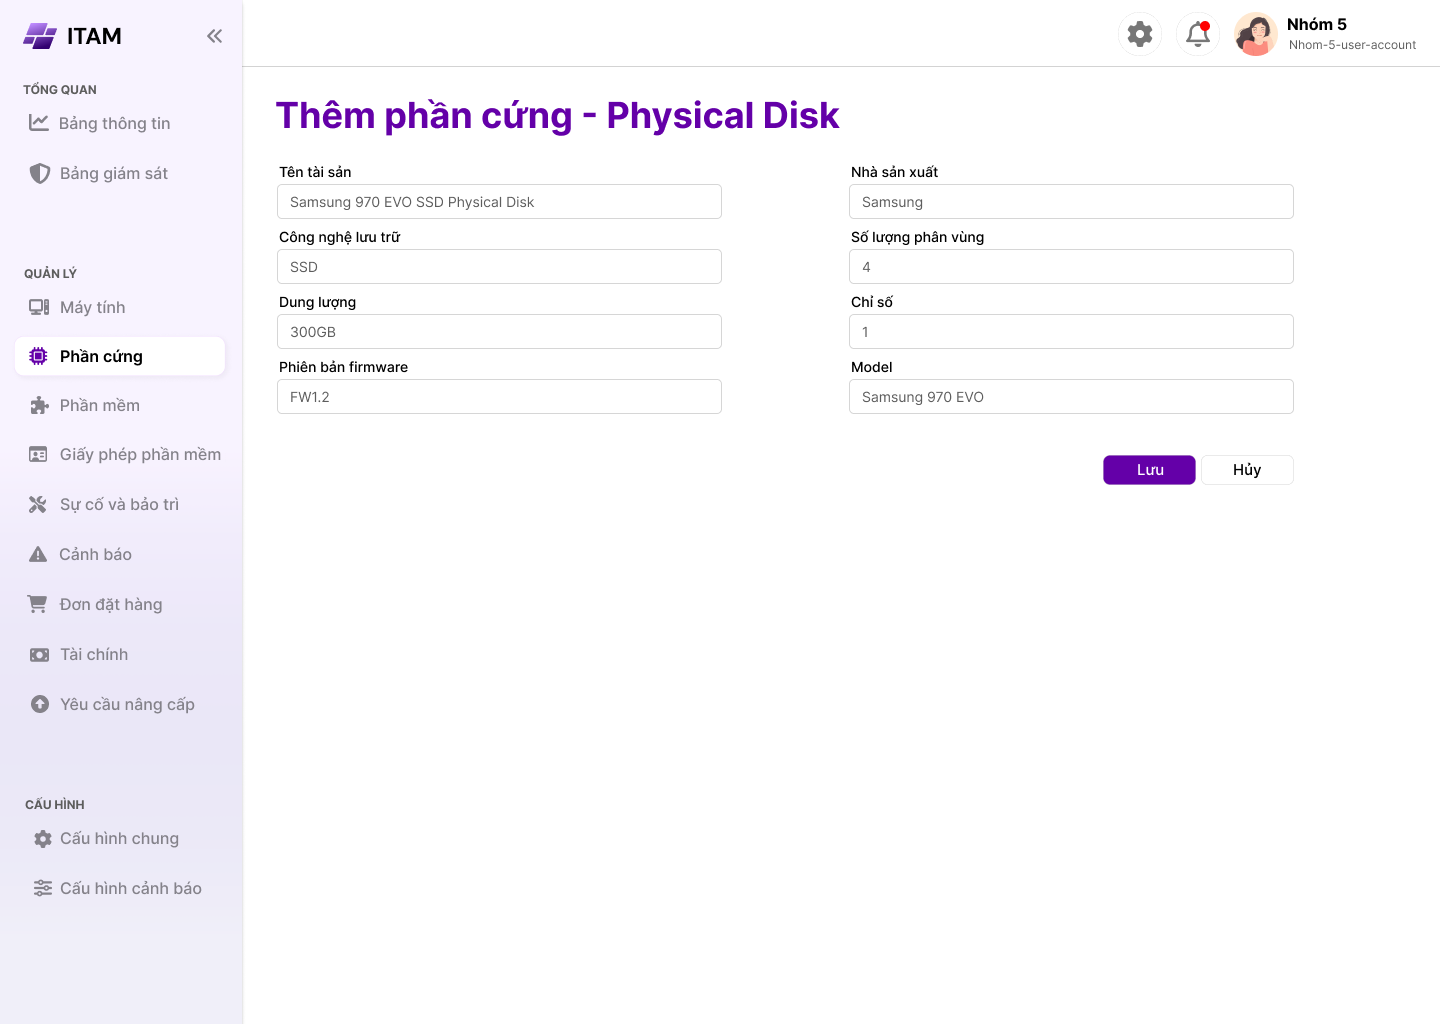
\includegraphics[width=14cm]{Images/C5/UI/Feature-Giám sát tài sản-Phần cứng 4.5.png}
%     \vspace{15pt}
%     \caption{Giao diện Quản lý phần cứng 8}
% \end{figure}
% \begin{figure}[H]
%     \centering
%     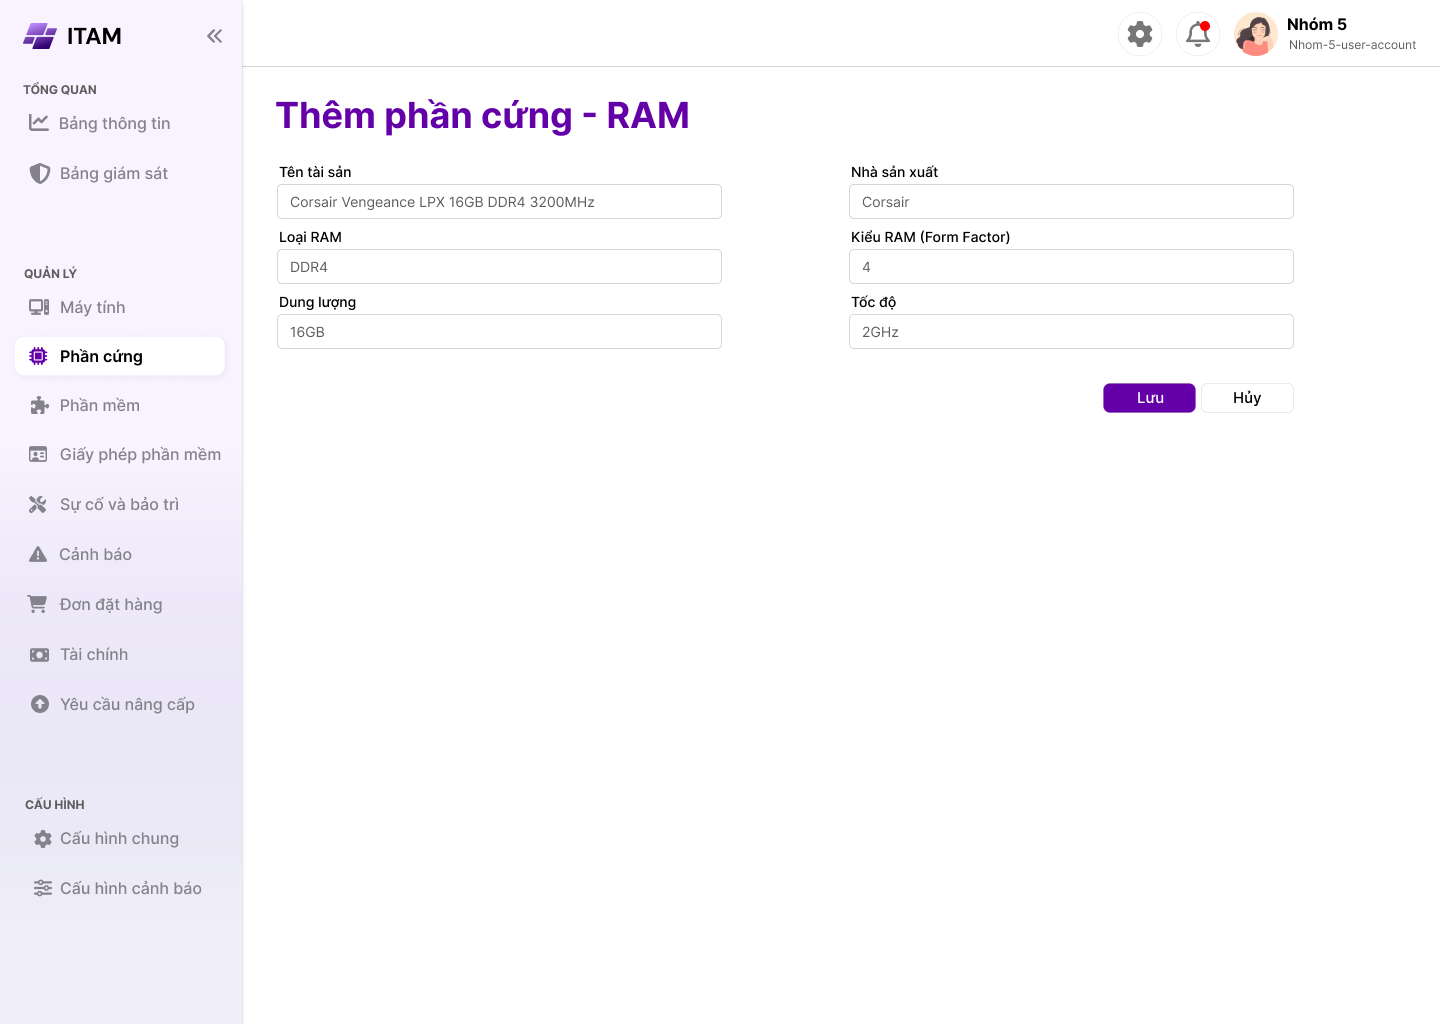
\includegraphics[width=14cm]{Images/C5/UI/Feature-Giám sát tài sản-Phần cứng 4.6.png}
%     \vspace{15pt}
%     \caption{Giao diện Quản lý phần cứng 9}
% \end{figure}
% \begin{figure}[H]
%     \centering
%     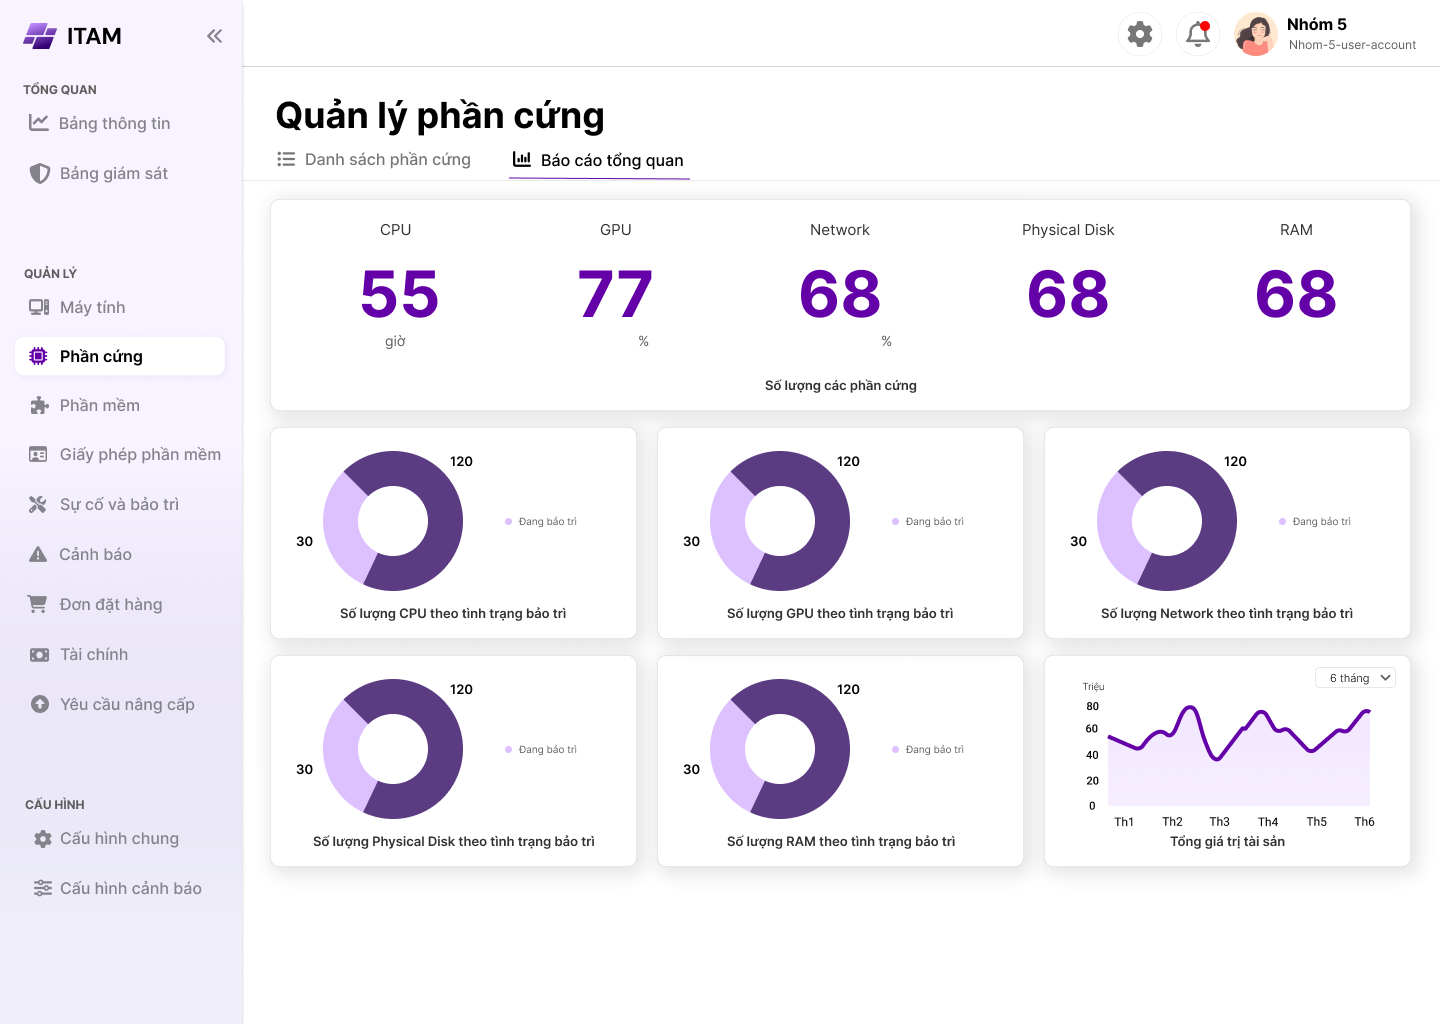
\includegraphics[width=14cm]{Images/C5/UI/Feature-Giám sát tài sản-Phần cứng 3.png}
%     \vspace{15pt}
%     \caption{Giao diện Quản lý phần cứng 4}
% \end{figure}

\item{Quản lý phần mềm}\\
Ở chức năng Quản lý phần mềm, người dùng có thể dễ dàng xem danh sách tất cả các phần mềm trong hệ thống, thêm mới phần mềm, xem chi tiết phần mềm, và xem báo cáo tổng quan về phần mềm (xem thêm chi tiết ở phụ lục).
% \begin{figure}[H]
%     \centering
%     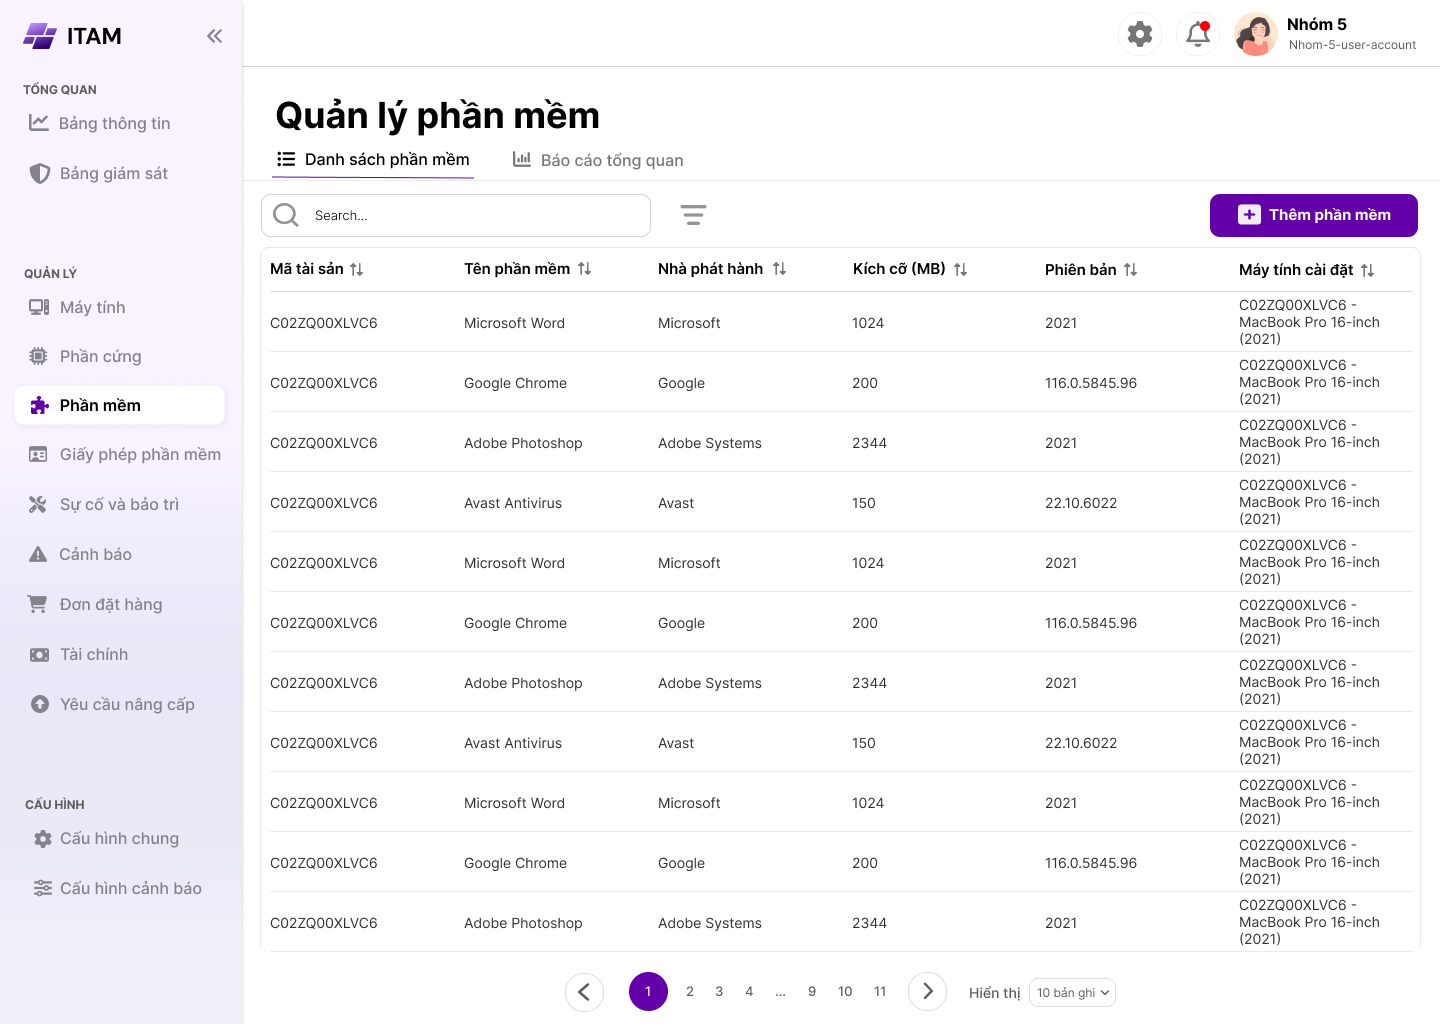
\includegraphics[width=14cm]{Images/C5/UI/Feature-Giám sát tài sản-Phần mềm 1.png}
%     \vspace{15pt}
%     \caption{Giao diện Quản lý phần mềm 1}
% \end{figure}
% \begin{figure}[H]
%     \centering
%     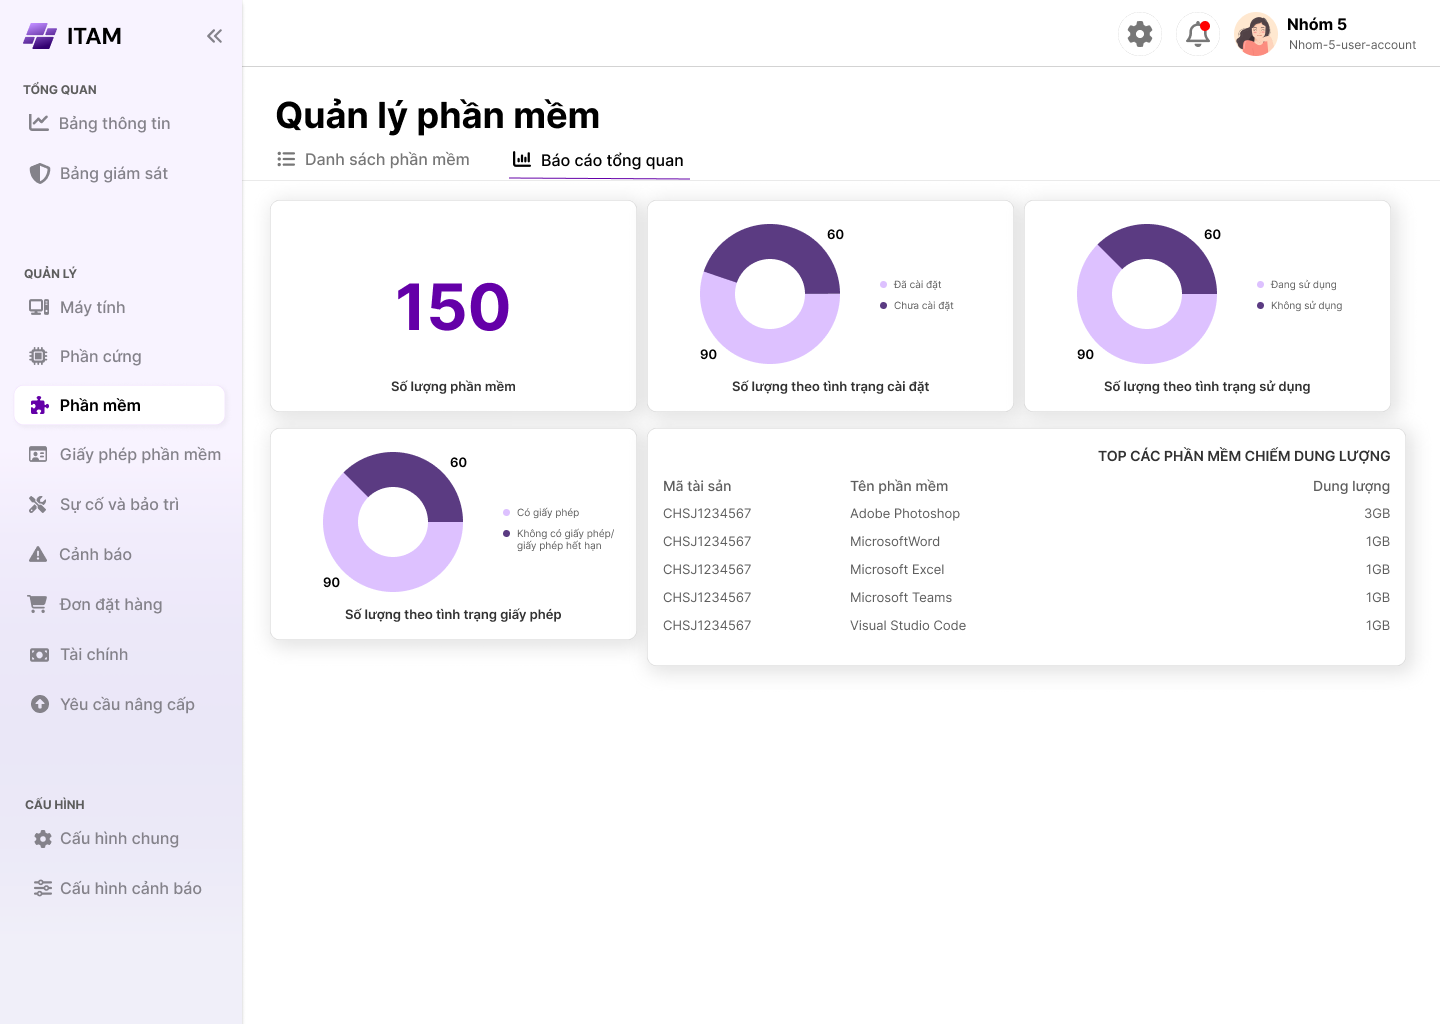
\includegraphics[width=14cm]{Images/C5/UI/Feature-Giám sát tài sản-Phần mềm 2.png}
%     \vspace{15pt}
%     \caption{Giao diện Quản lý phần mềm 2}
% \end{figure}
% \begin{figure}[H]
%     \centering
%     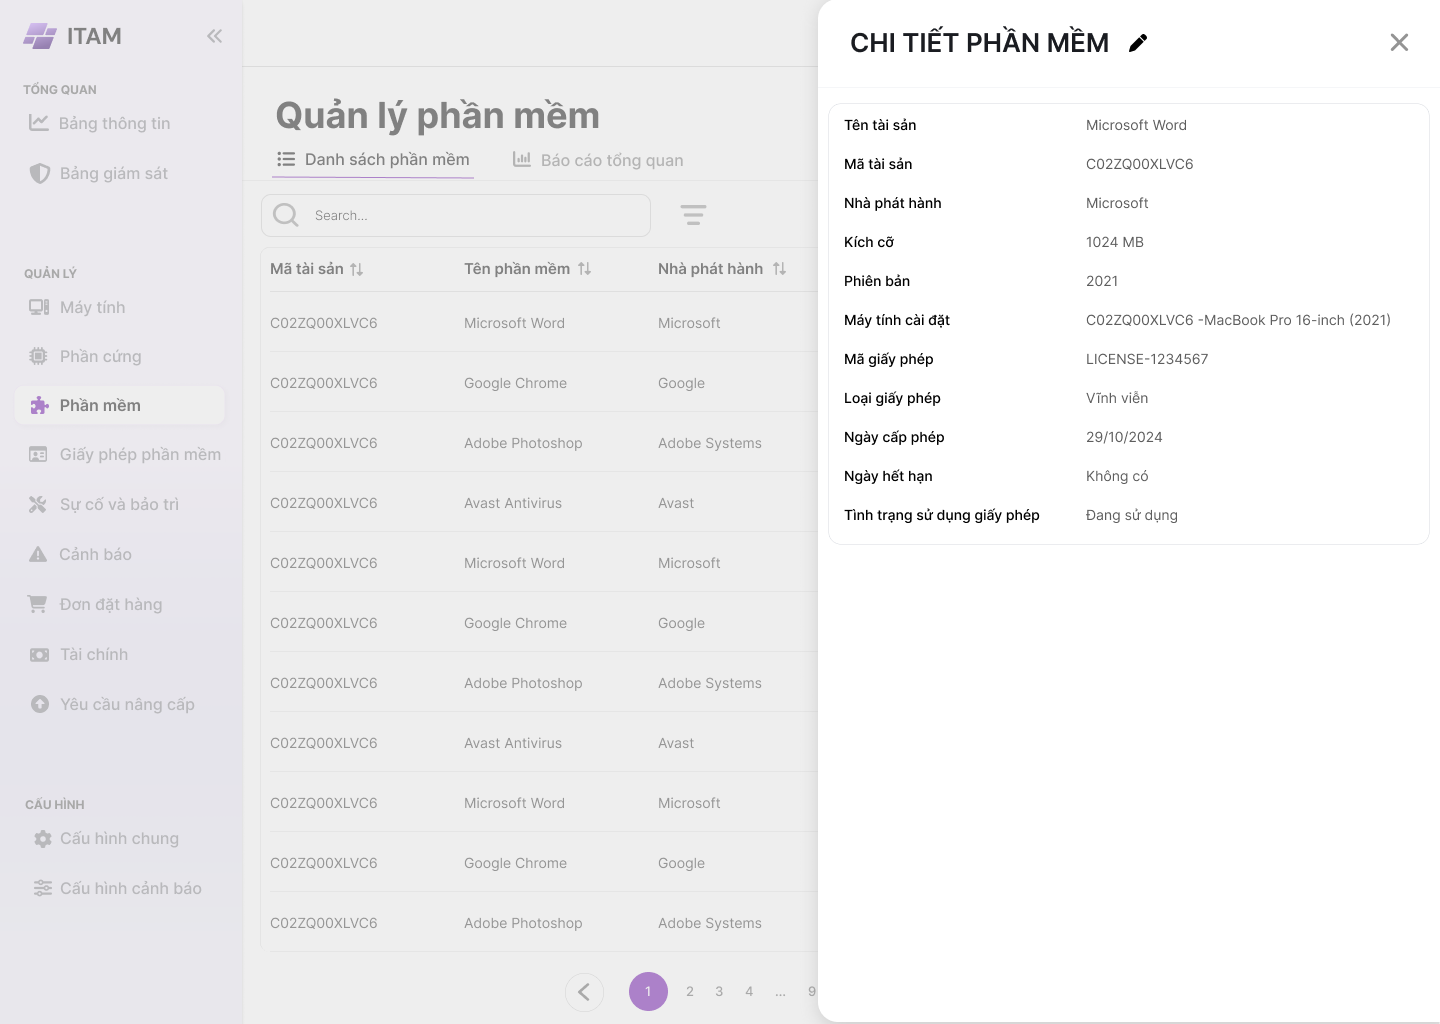
\includegraphics[width=14cm]{Images/C5/UI/Feature-Giám sát tài sản-Phần mềm 3.png}
%     \vspace{15pt}
%     \caption{Giao diện Quản lý phần mềm 3}
% \end{figure}
% \begin{figure}[H]
%     \centering
%     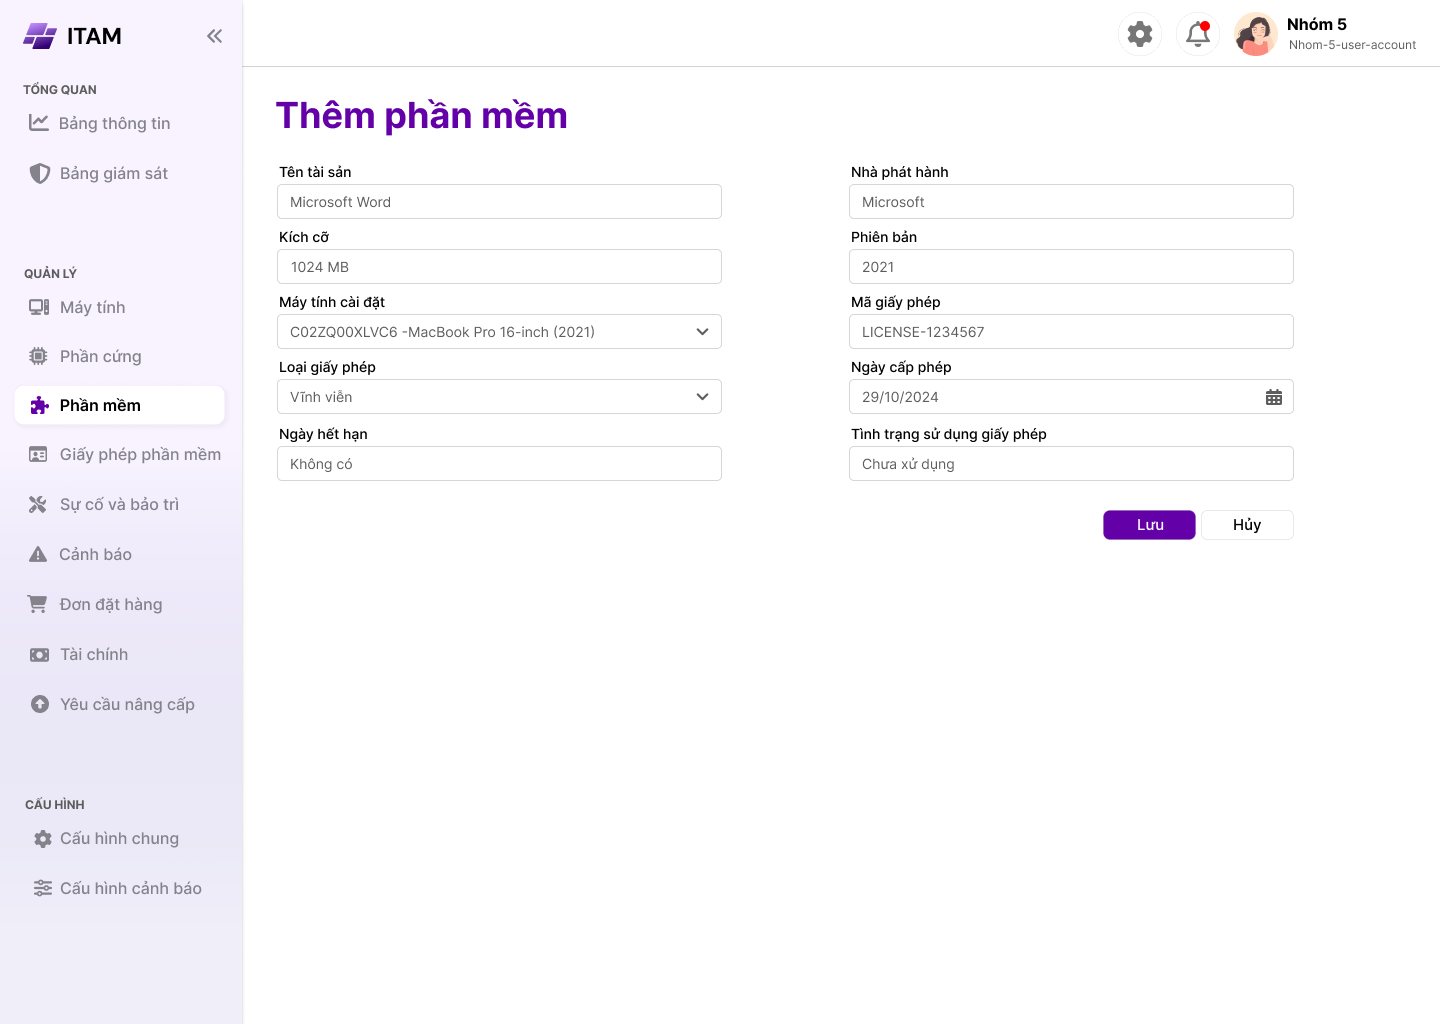
\includegraphics[width=14cm]{Images/C5/UI/Feature-Giám sát tài sản-Phần mềm 4.png}
%     \vspace{15pt}
%     \caption{Giao diện Quản lý phần mềm 4}
% \end{figure}

\item{Quản lý sự cố và bảo trì}\\
Quản lý sự cố và bảo trì cung cấp các tính năng xem danh sách, chi tiết sự cố và yêu cầu bảo trì của tài sản, giúp người dùng có thể quản lý một cách tập trung sự cố và bảo trì trong hệ thống (xem thêm chi tiết ở phụ lục).
% \begin{figure}[H]
%     \centering
%     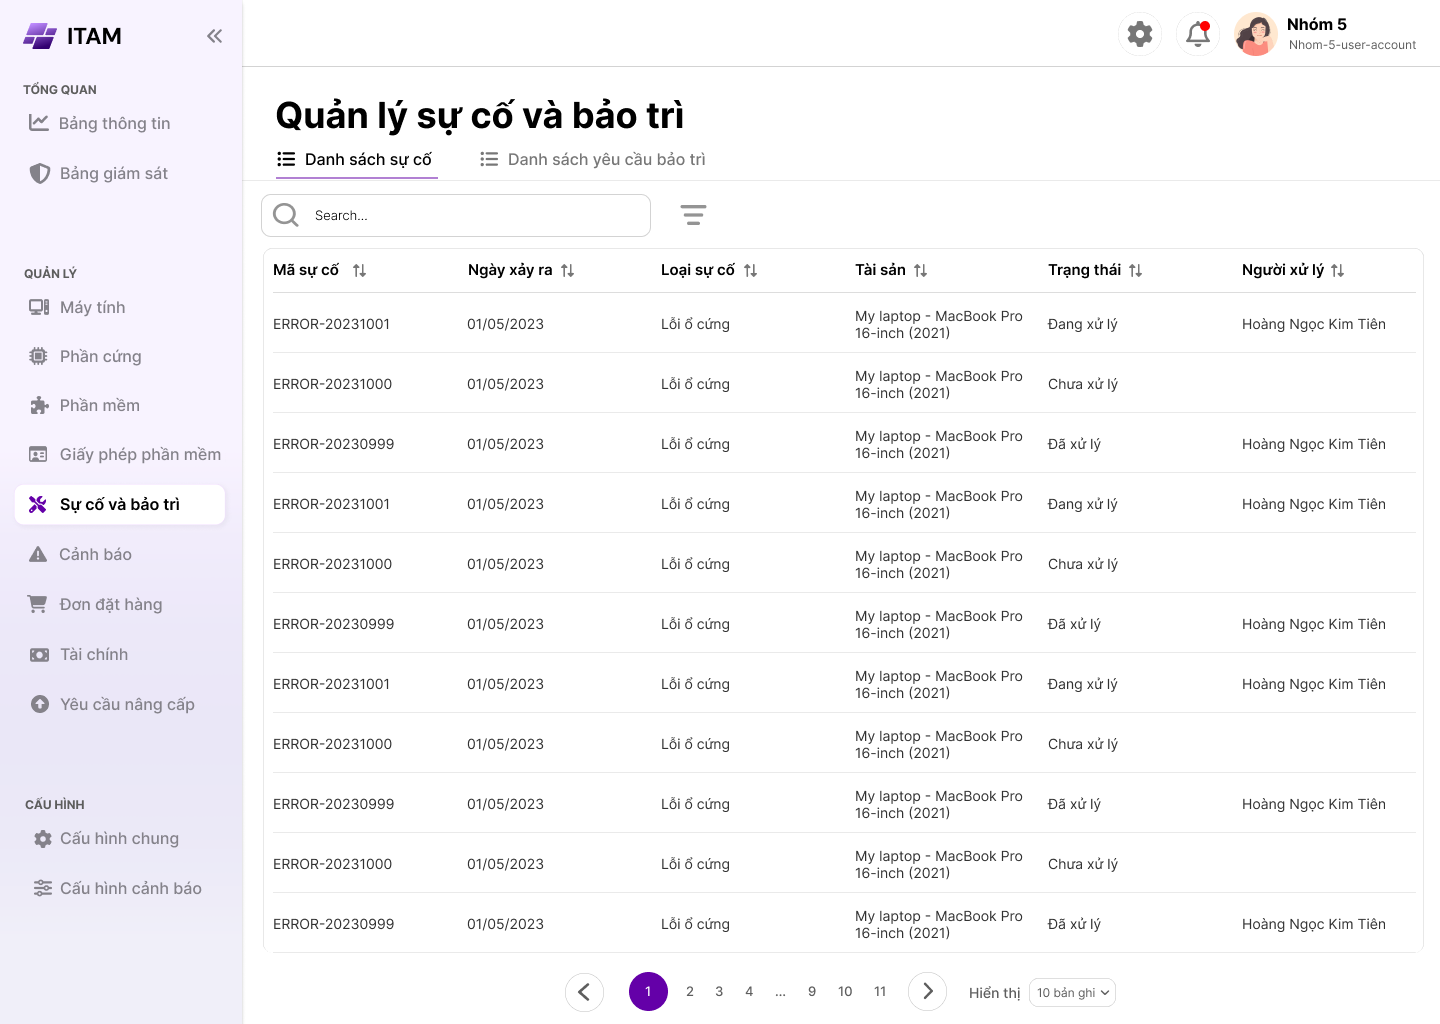
\includegraphics[width=14cm]{Images/C5/UI/Feature-Quản lý sự cố và bảo trì 1.png}
%     \vspace{15pt}
%     \caption{Giao diện Quản lý sự cố và bảo trì 1}
% \end{figure}
% \begin{figure}[H]
%     \centering
%     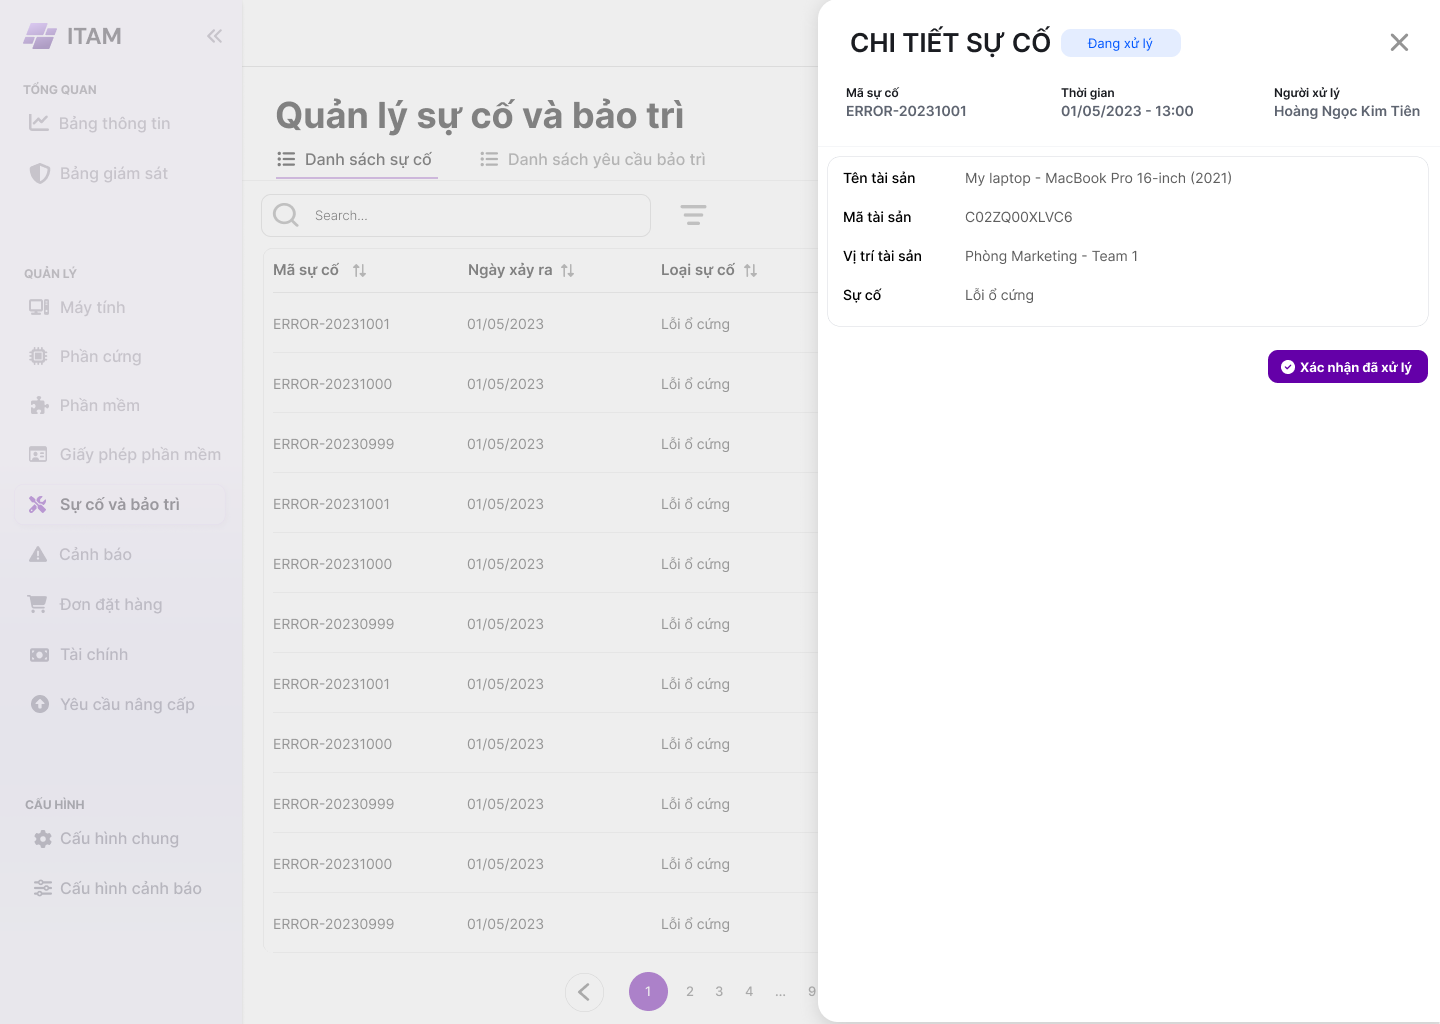
\includegraphics[width=14cm]{Images/C5/UI/Feature-Quản lý sự cố và bảo trì 2.1.png}
%     \vspace{15pt}
%     \caption{Giao diện Quản lý sự cố và bảo trì 2}
% \end{figure}
% \begin{figure}[H]
%     \centering
%     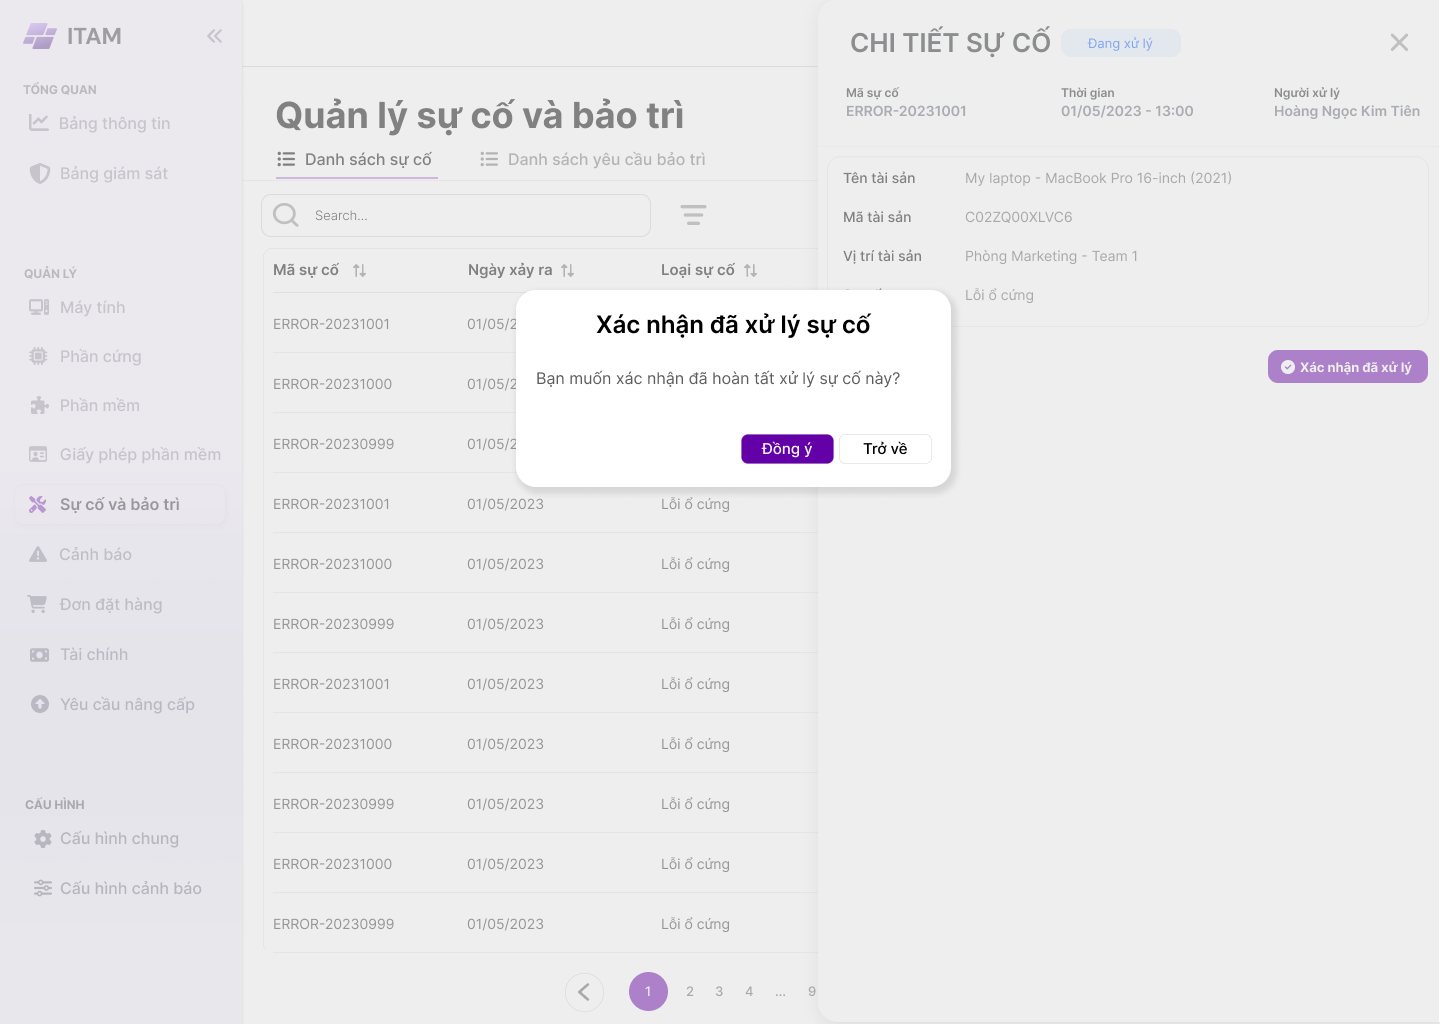
\includegraphics[width=14cm]{Images/C5/UI/Feature-Quản lý sự cố và bảo trì 2.2.png}
%     \vspace{15pt}
%     \caption{Giao diện Quản lý sự cố và bảo trì 3}
% \end{figure}
% \begin{figure}[H]
%     \centering
%     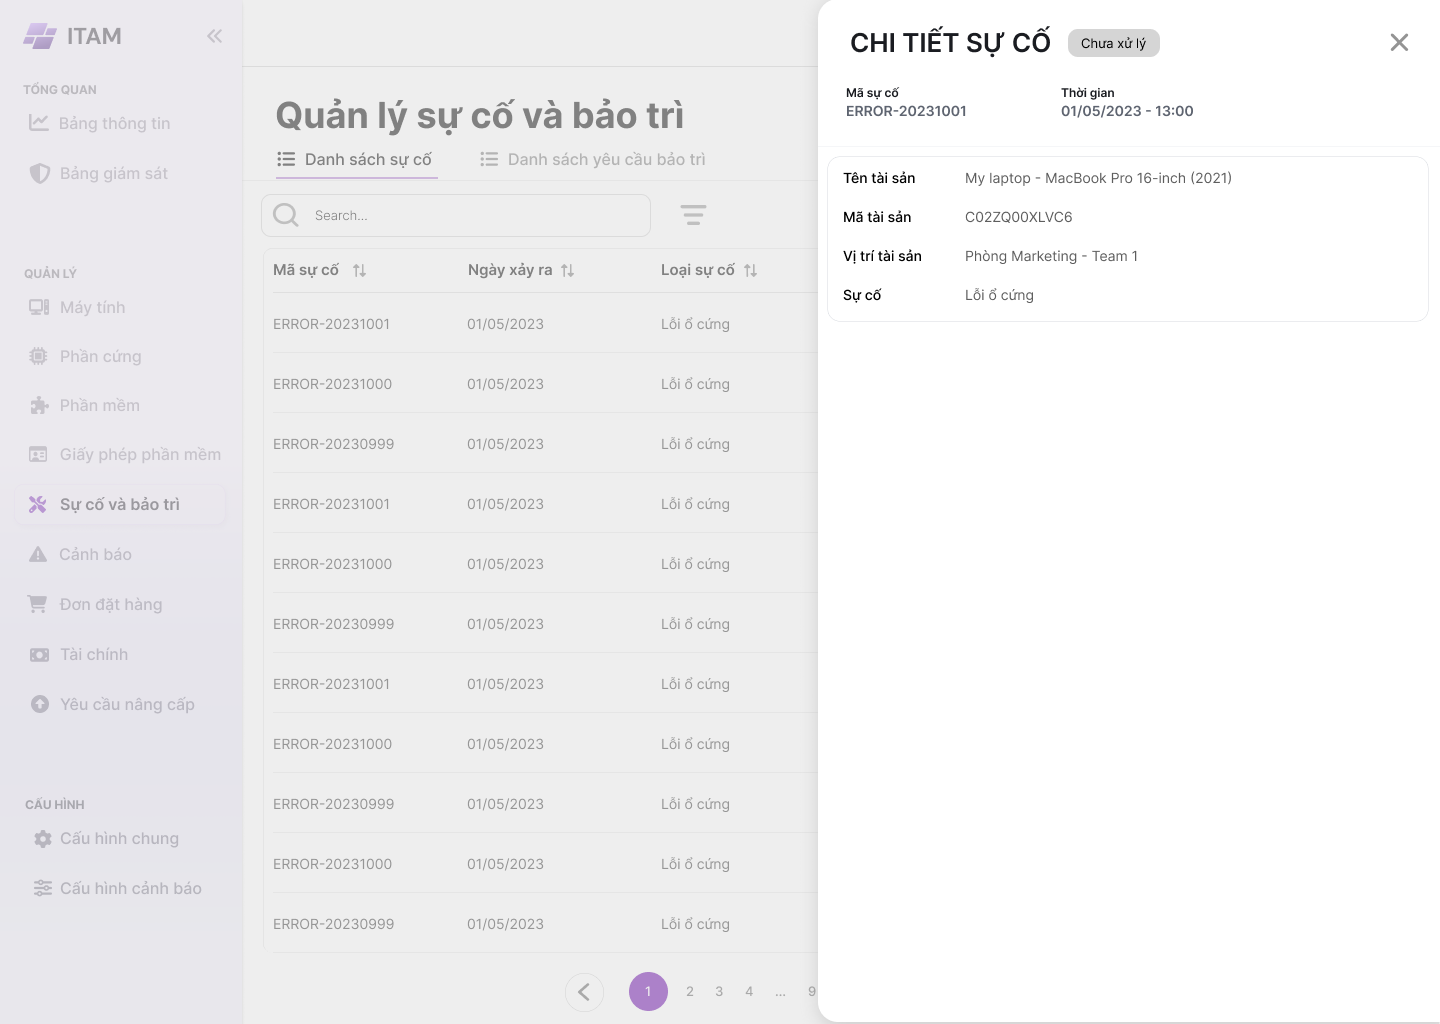
\includegraphics[width=14cm]{Images/C5/UI/Feature-Quản lý sự cố và bảo trì 2.3.png}
%     \vspace{15pt}
%     \caption{Giao diện Quản lý sự cố và bảo trì 4}
% \end{figure}
% \begin{figure}[H]
%     \centering
%     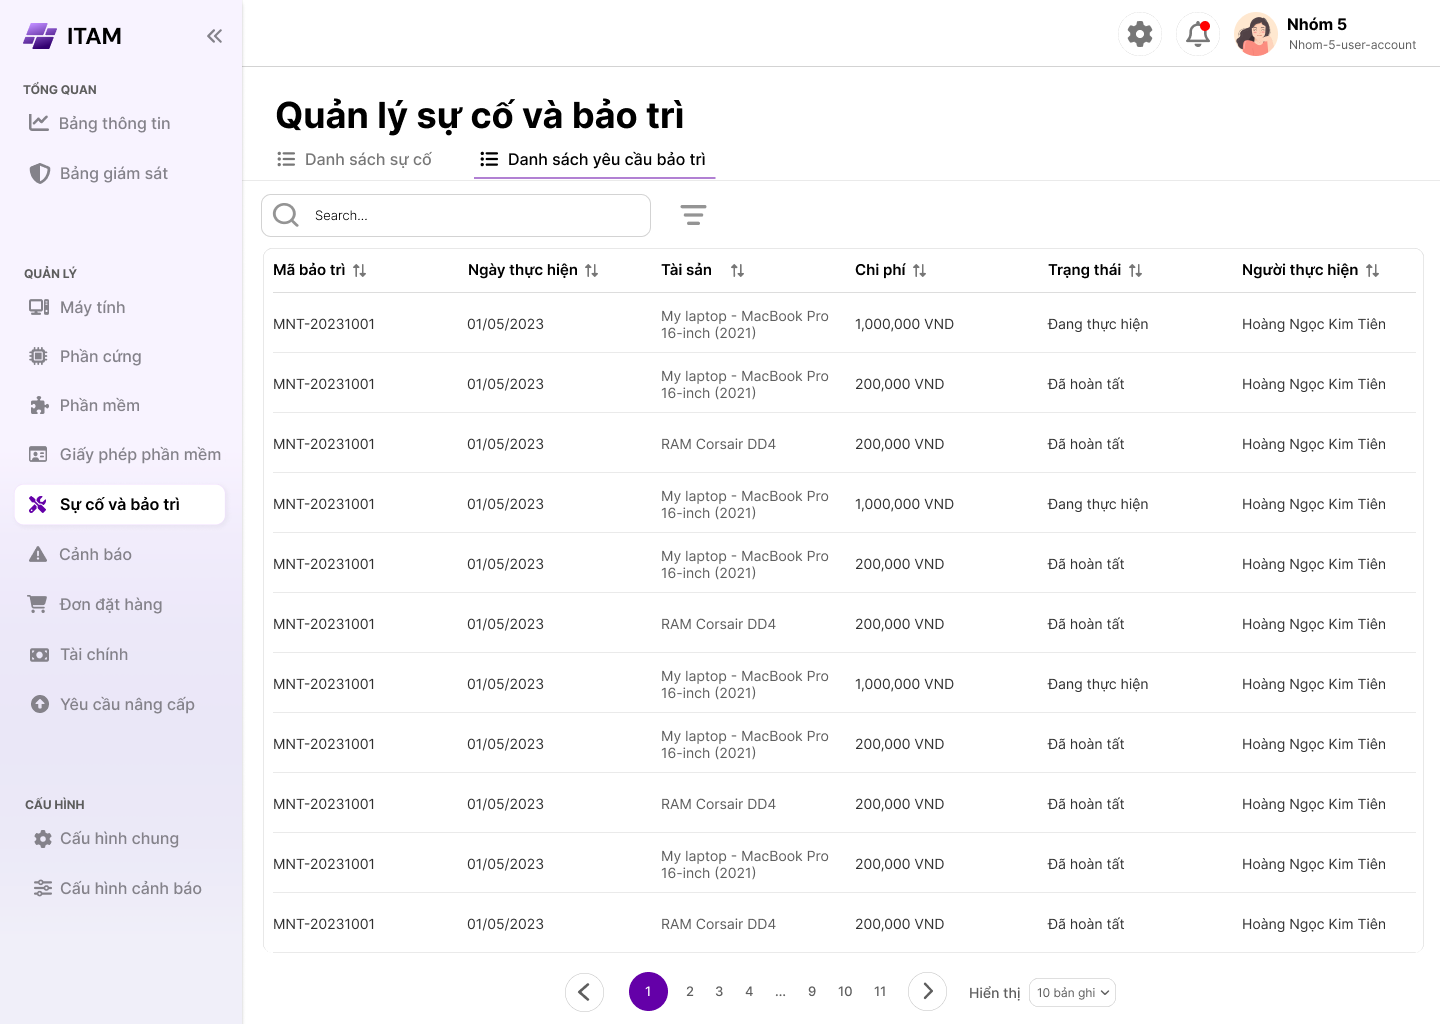
\includegraphics[width=14cm]{Images/C5/UI/Feature-Quản lý sự cố và bảo trì 3.1.png}
%     \vspace{15pt}
%     \caption{Giao diện Quản lý sự cố và bảo trì 3}
% \end{figure}
% \begin{figure}[H]
%     \centering
%     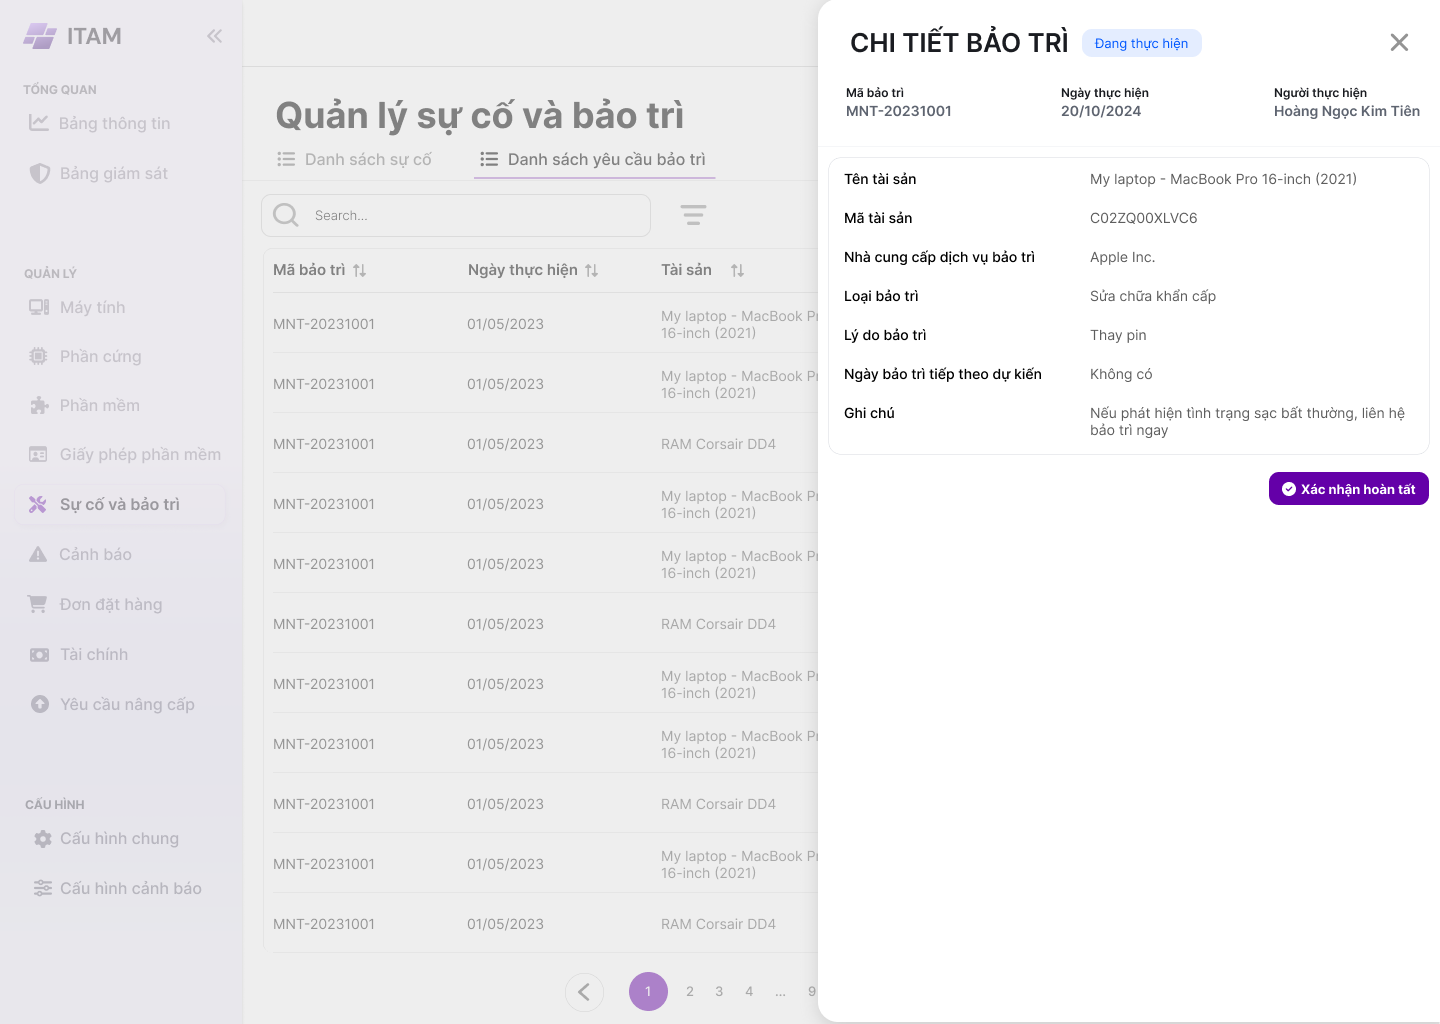
\includegraphics[width=14cm]{Images/C5/UI/Feature-Quản lý sự cố và bảo trì 3.2.png}
%     \vspace{15pt}
%     \caption{Giao diện Quản lý sự cố và bảo trì 4}
% \end{figure}
% \begin{figure}[H]
%     \centering
%     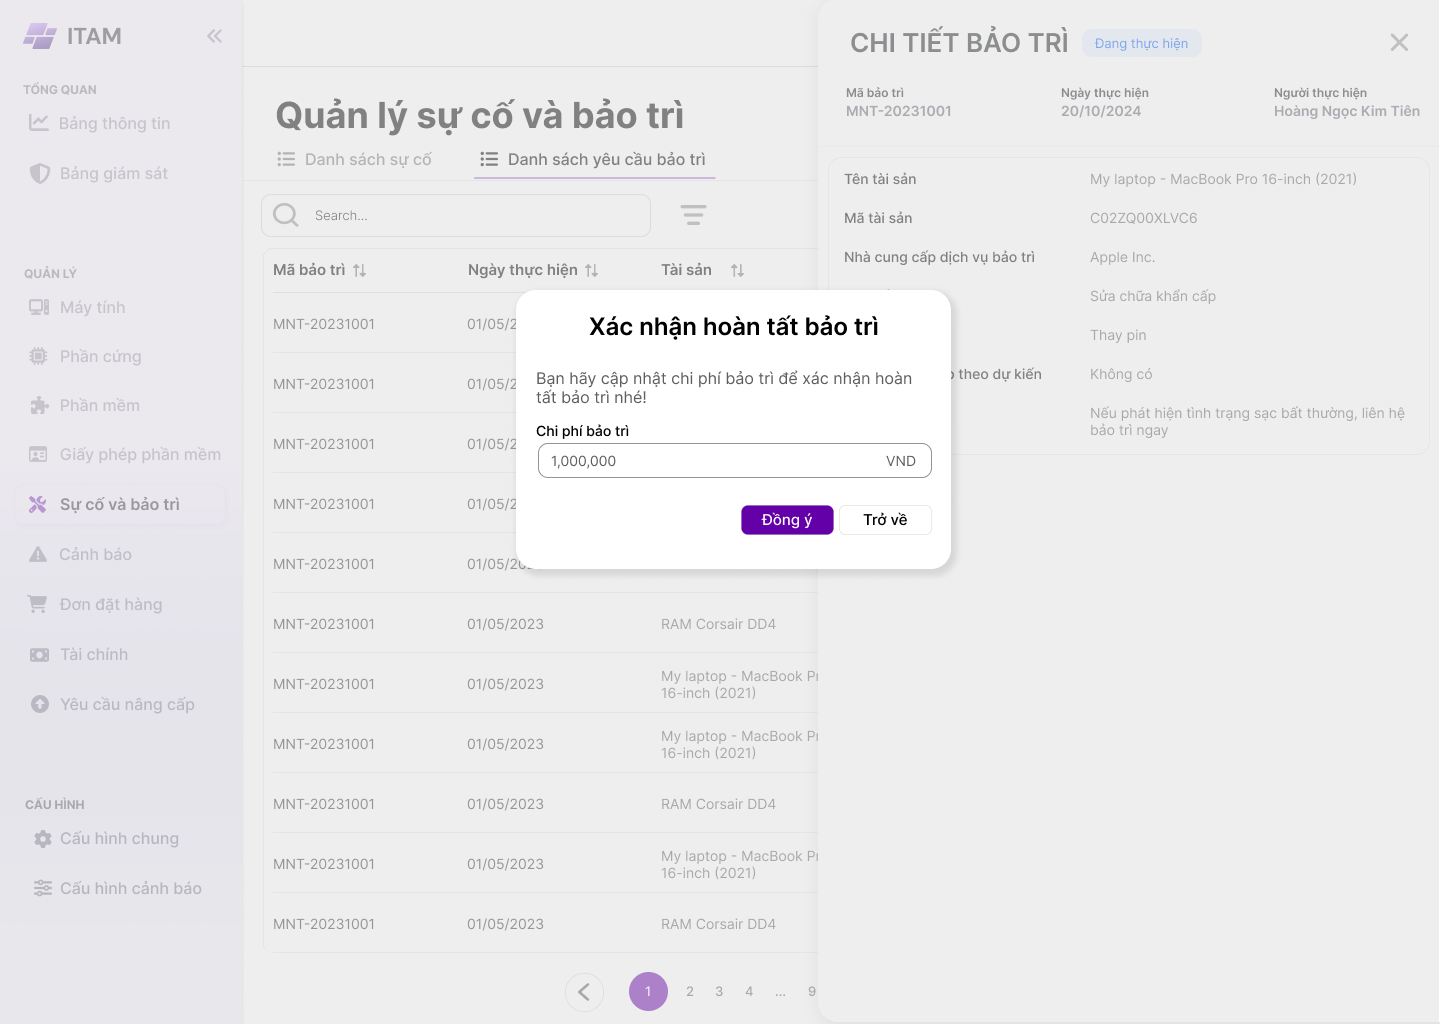
\includegraphics[width=14cm]{Images/C5/UI/Feature-Quản lý sự cố và bảo trì 3.3.png}
%     \vspace{15pt}
%     \caption{Giao diện Quản lý sự cố và bảo trì 7}
% \end{figure}

\item{Quản lý cảnh báo}\\
Ở Quản lý cảnh báo, người cùng có thể xem tất cả các cảnh báo của các máy tính có trong hệ thống và xem chi tiết các cảnh báo đó. Cảnh báo cũng được phân loại màu sắc dựa trên mức độ nghiêm trọng để người dùng có thể kịp thời đưa ra quyết định xử lý các cảnh báo quan trọng (xem thêm chi tiết ở phụ lục).
% \begin{figure}[H]
%     \centering
%     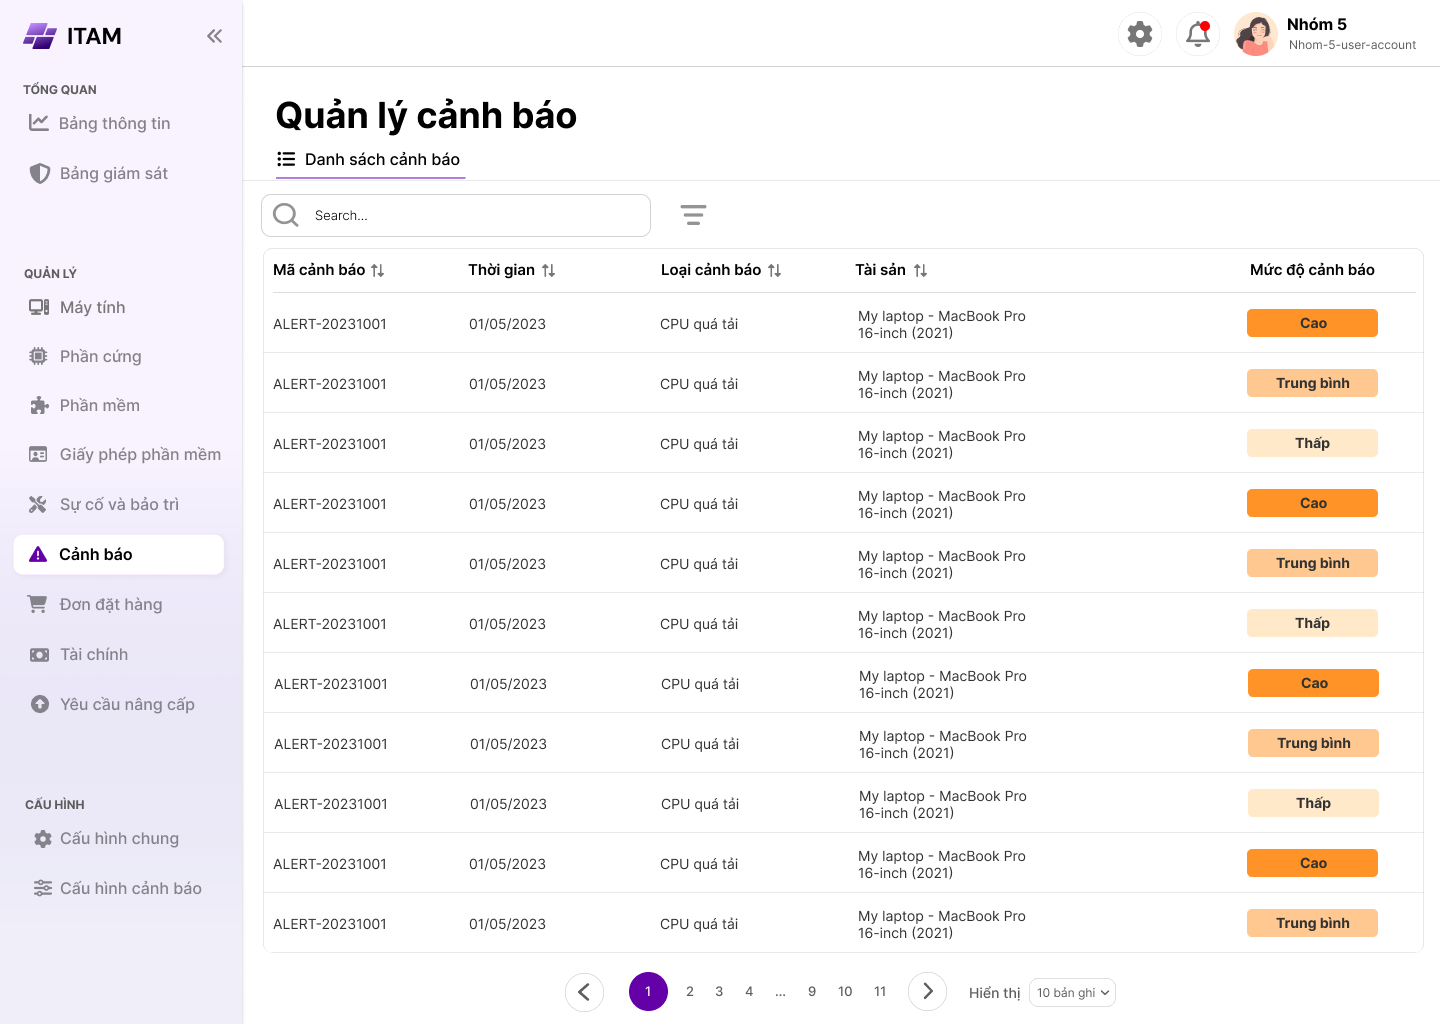
\includegraphics[width=14cm]{Images/C5/UI/Feature-Quản lý cảnh báo 1.png}
%     \vspace{15pt}
%     \caption{Giao diện Quản lý cảnh báo 1}
% \end{figure}
% \begin{figure}[H]
%     \centering
%     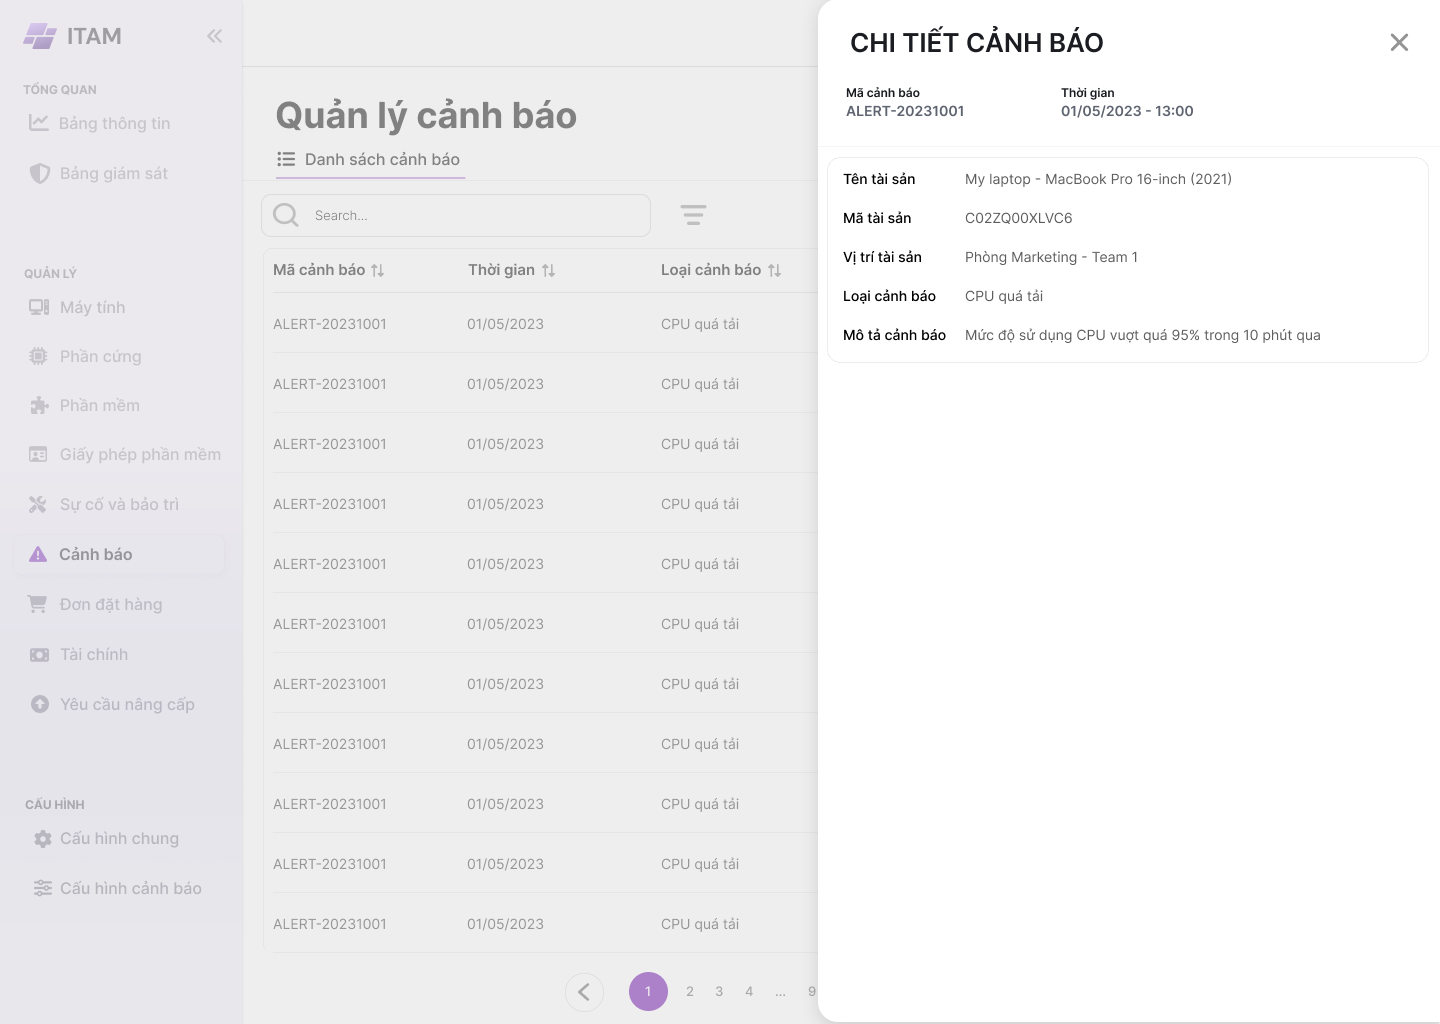
\includegraphics[width=14cm]{Images/C5/UI/Feature-Quản lý cảnh báo 2.1.png}
%     \vspace{15pt}
%     \caption{Giao diện Quản lý cảnh báo 2}
% \end{figure}

\item{Quản lý yêu cầu nâng cấp}\\
Người dùng có thể xem danh sách các yêu cầu nâng cấp và chi tiết các yêu cầu nâng cấp đó, đồng thời quản lý cũng có thể phê duyệt các yêu cầu nâng cấp (xem thêm chi tiết ở phụ lục).
% \begin{figure}[H]
%     \centering
%     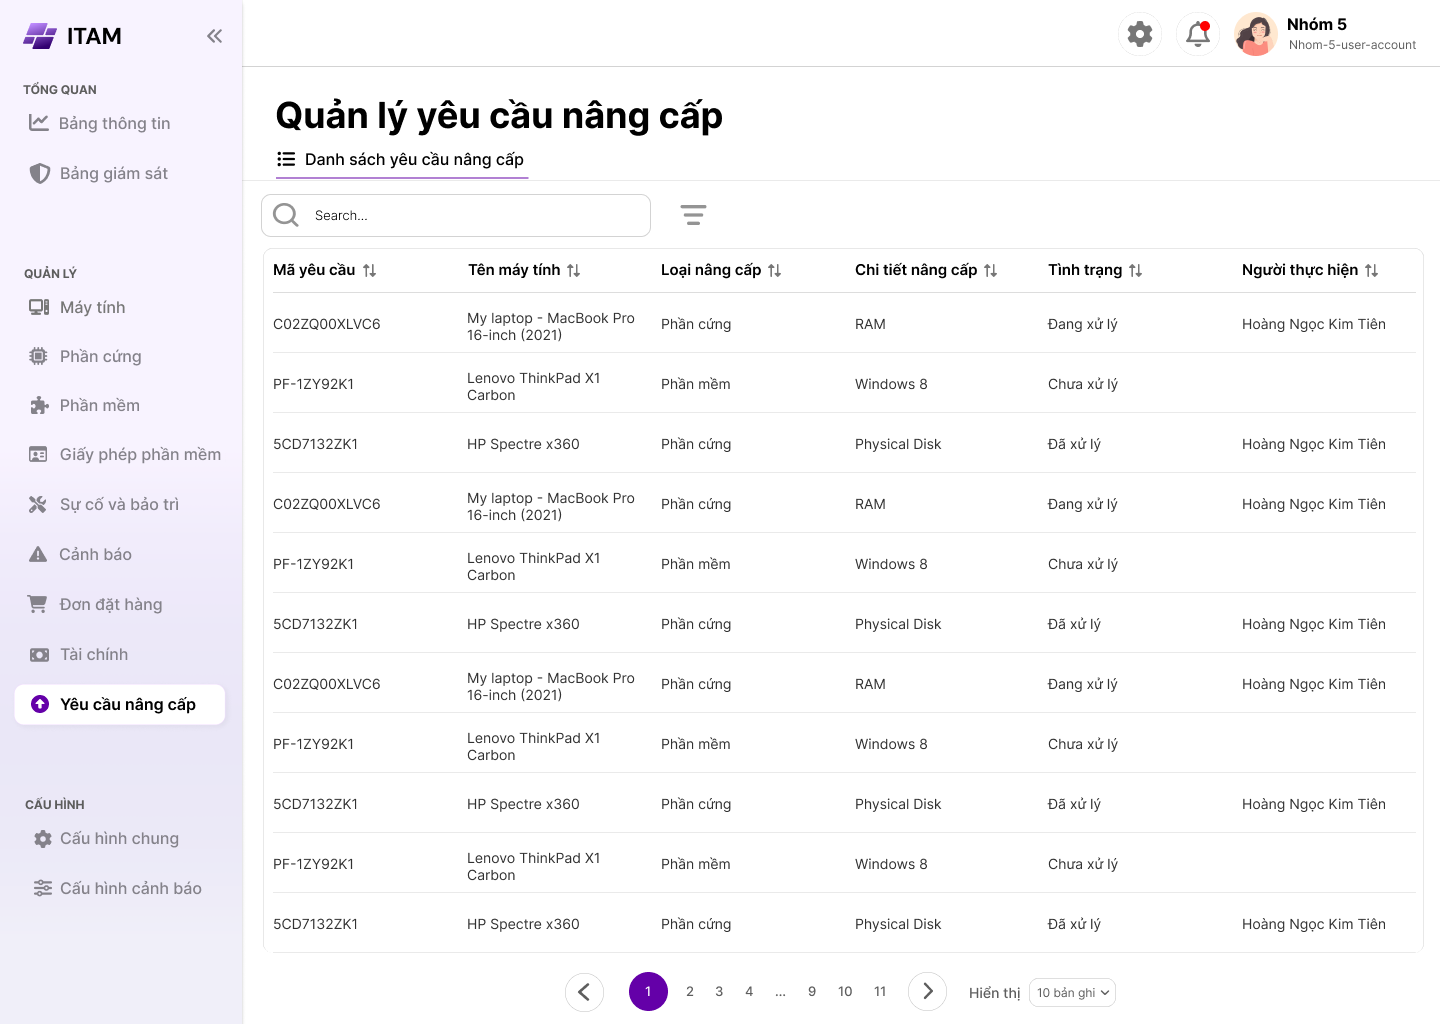
\includegraphics[width=14cm]{Images/C5/UI/Feature-Quản lý yêu cầu nâng cấp 1.png}
%     \vspace{15pt}
%     \caption{Giao diện Quản lý yêu cầu nâng cấp 1}
% \end{figure}
% \begin{figure}[H]
%     \centering
%     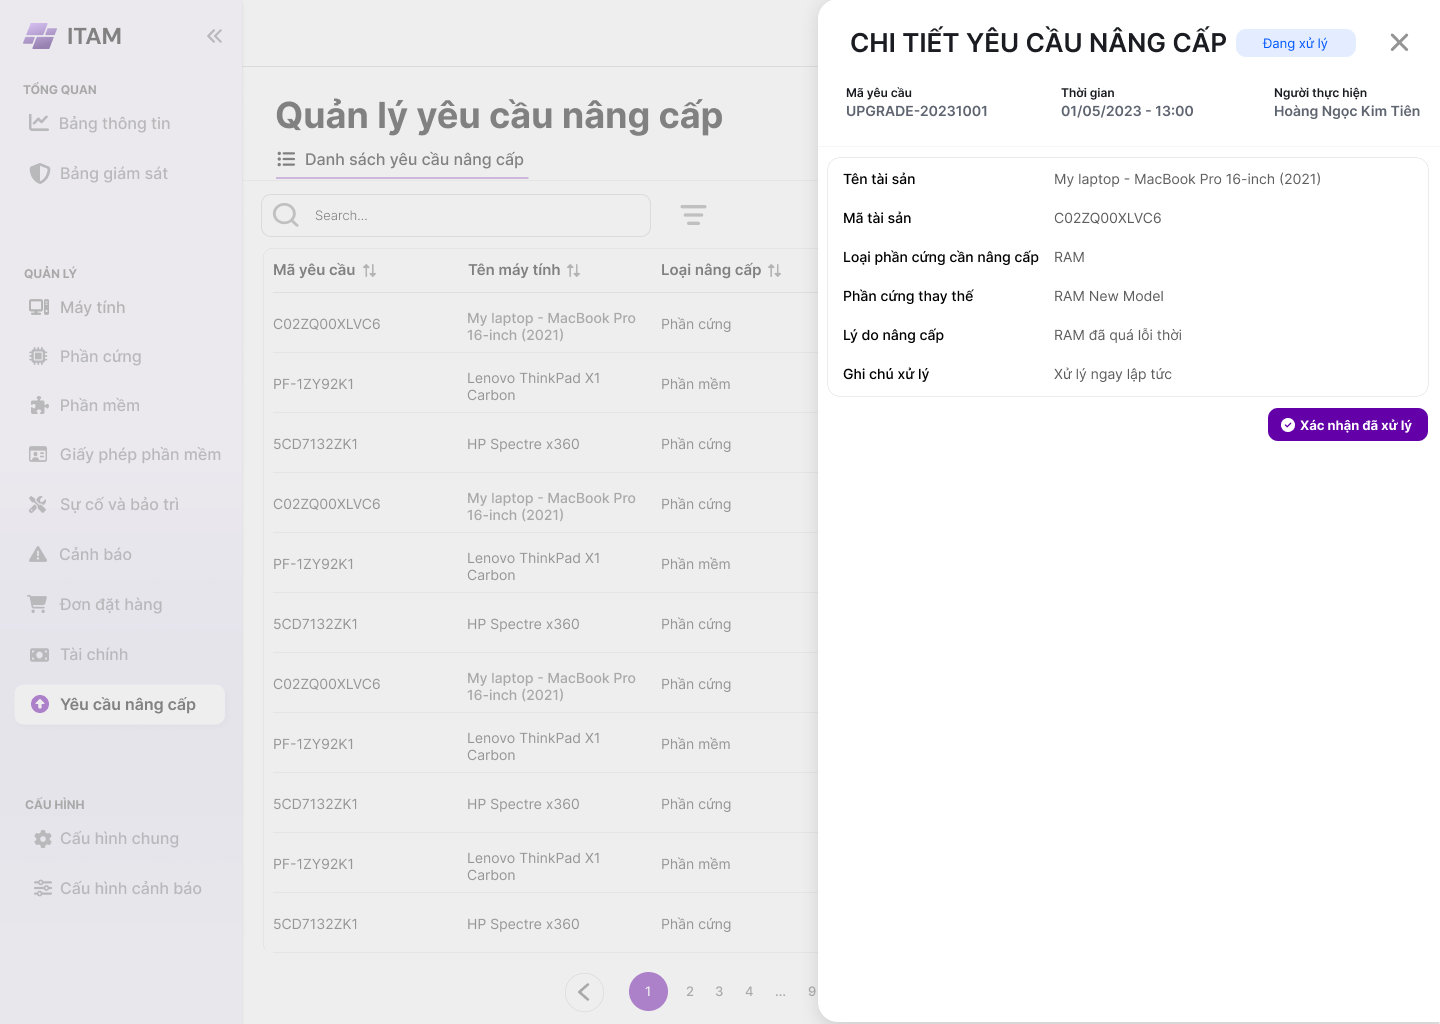
\includegraphics[width=14cm]{Images/C5/UI/Feature-Quản lý yêu cầu nâng cấp 2.1.png}
%     \vspace{15pt}
%     \caption{Giao diện Quản lý yêu cầu nâng cấp 2}
% \end{figure}
% \begin{figure}[H]
%     \centering
%     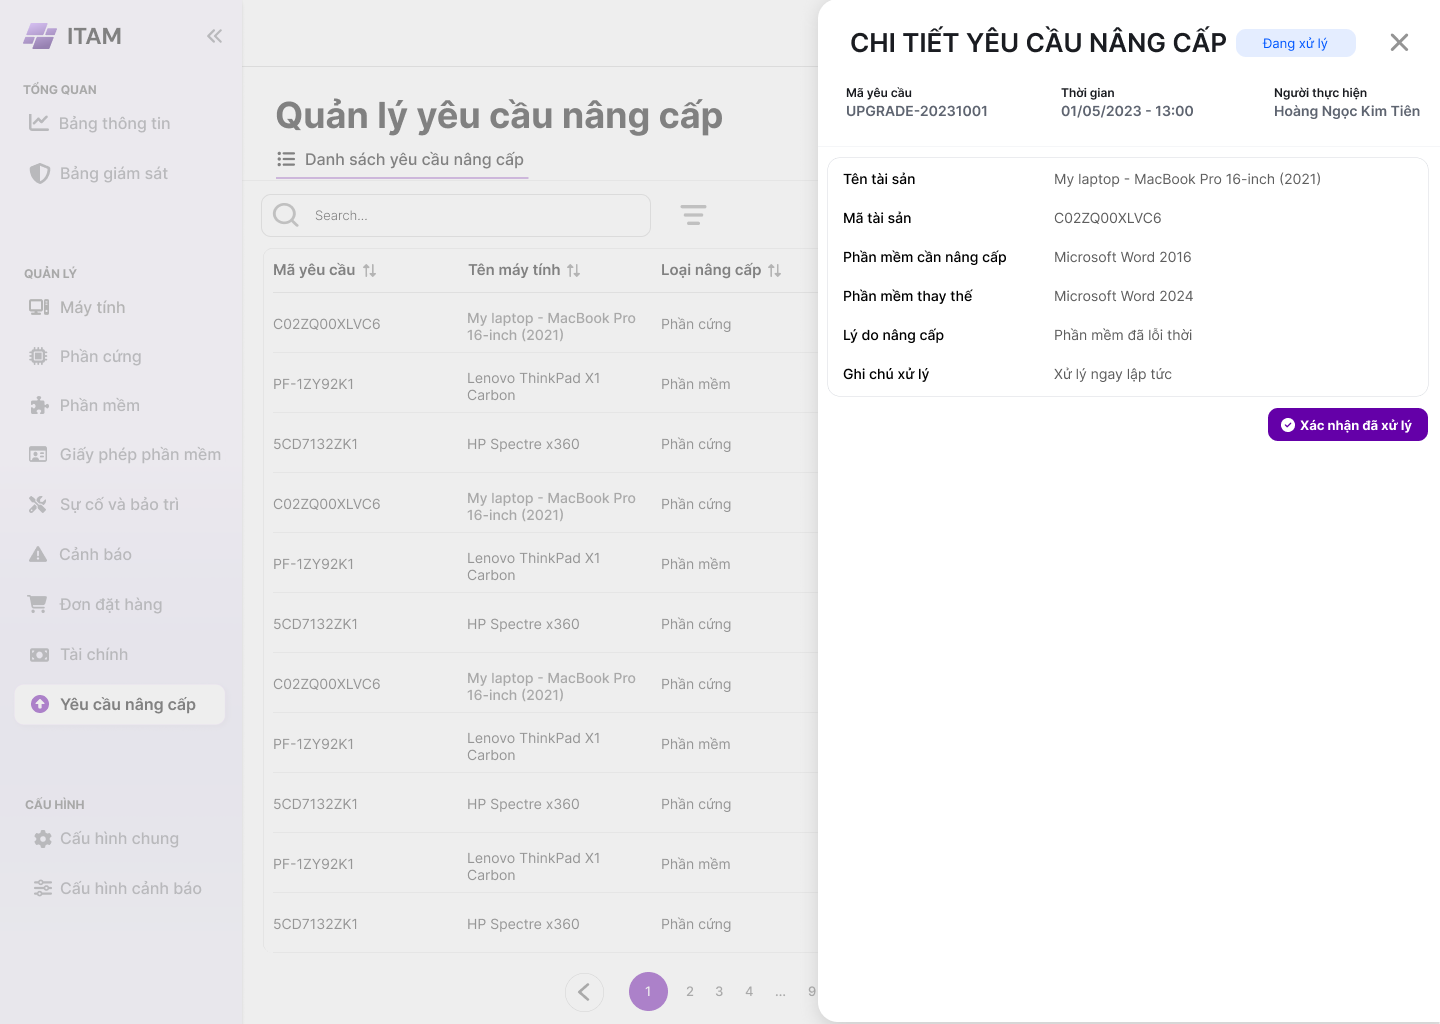
\includegraphics[width=14cm]{Images/C5/UI/Feature-Quản lý yêu cầu nâng cấp 2.2.png}
%     \vspace{15pt}
%     \caption{Giao diện Quản lý yêu cầu nâng cấp 3}
% \end{figure}
% \begin{figure}[H]
%     \centering
%     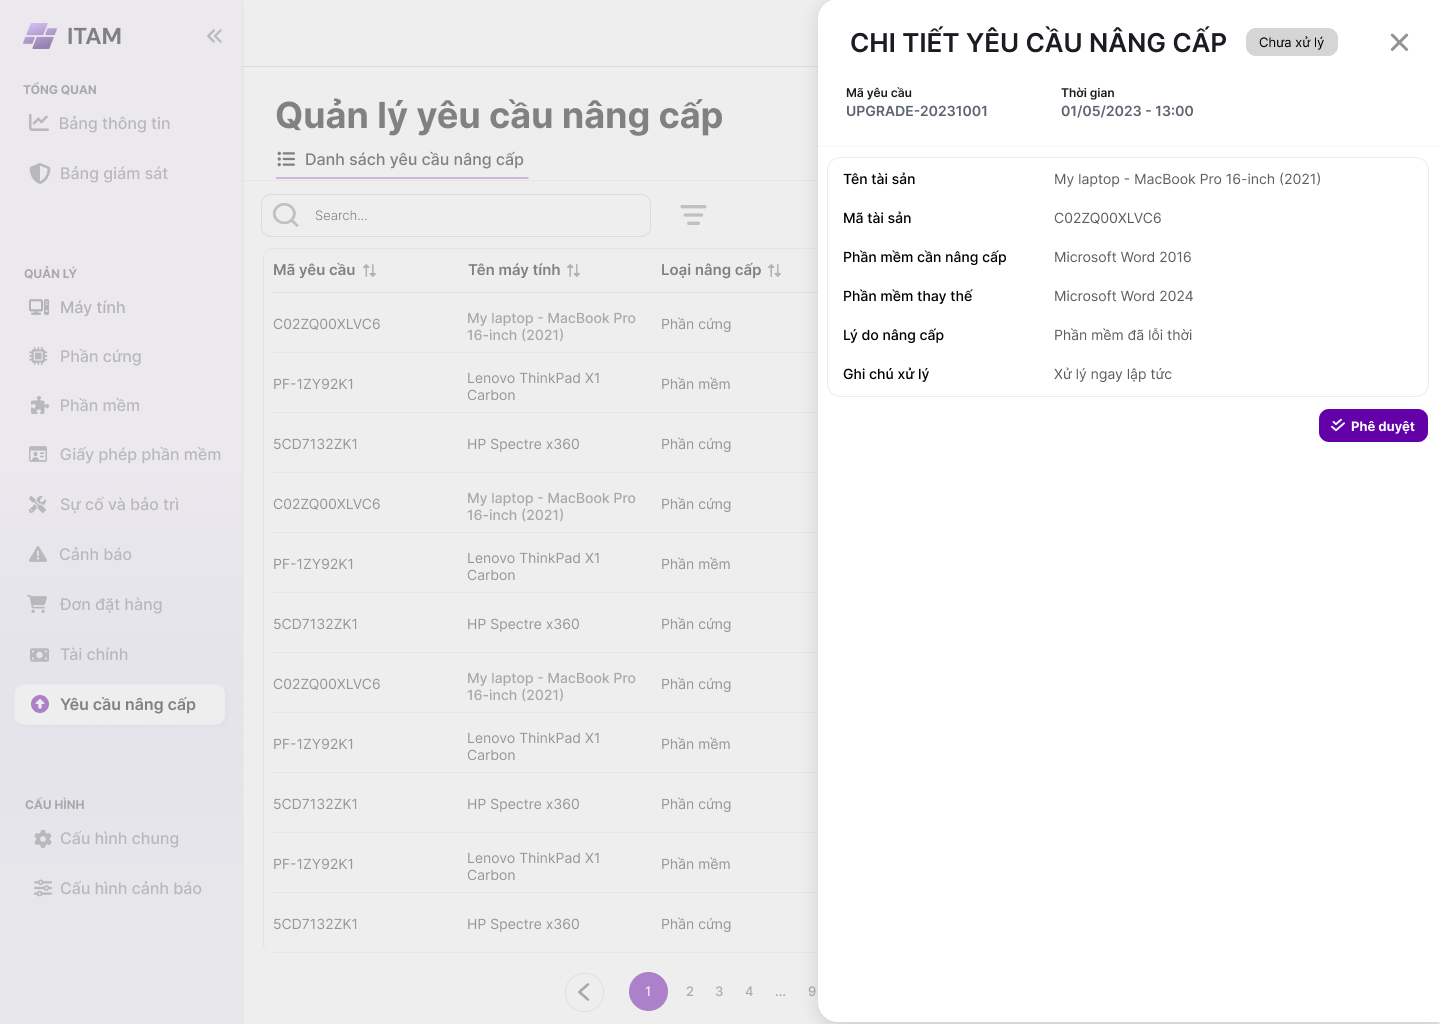
\includegraphics[width=14cm]{Images/C5/UI/Feature-Quản lý yêu cầu nâng cấp 2.3.png}
%     \vspace{15pt}
%     \caption{Giao diện Quản lý yêu cầu nâng cấp 2}
% \end{figure}
% \begin{figure}[H]
%     \centering
%     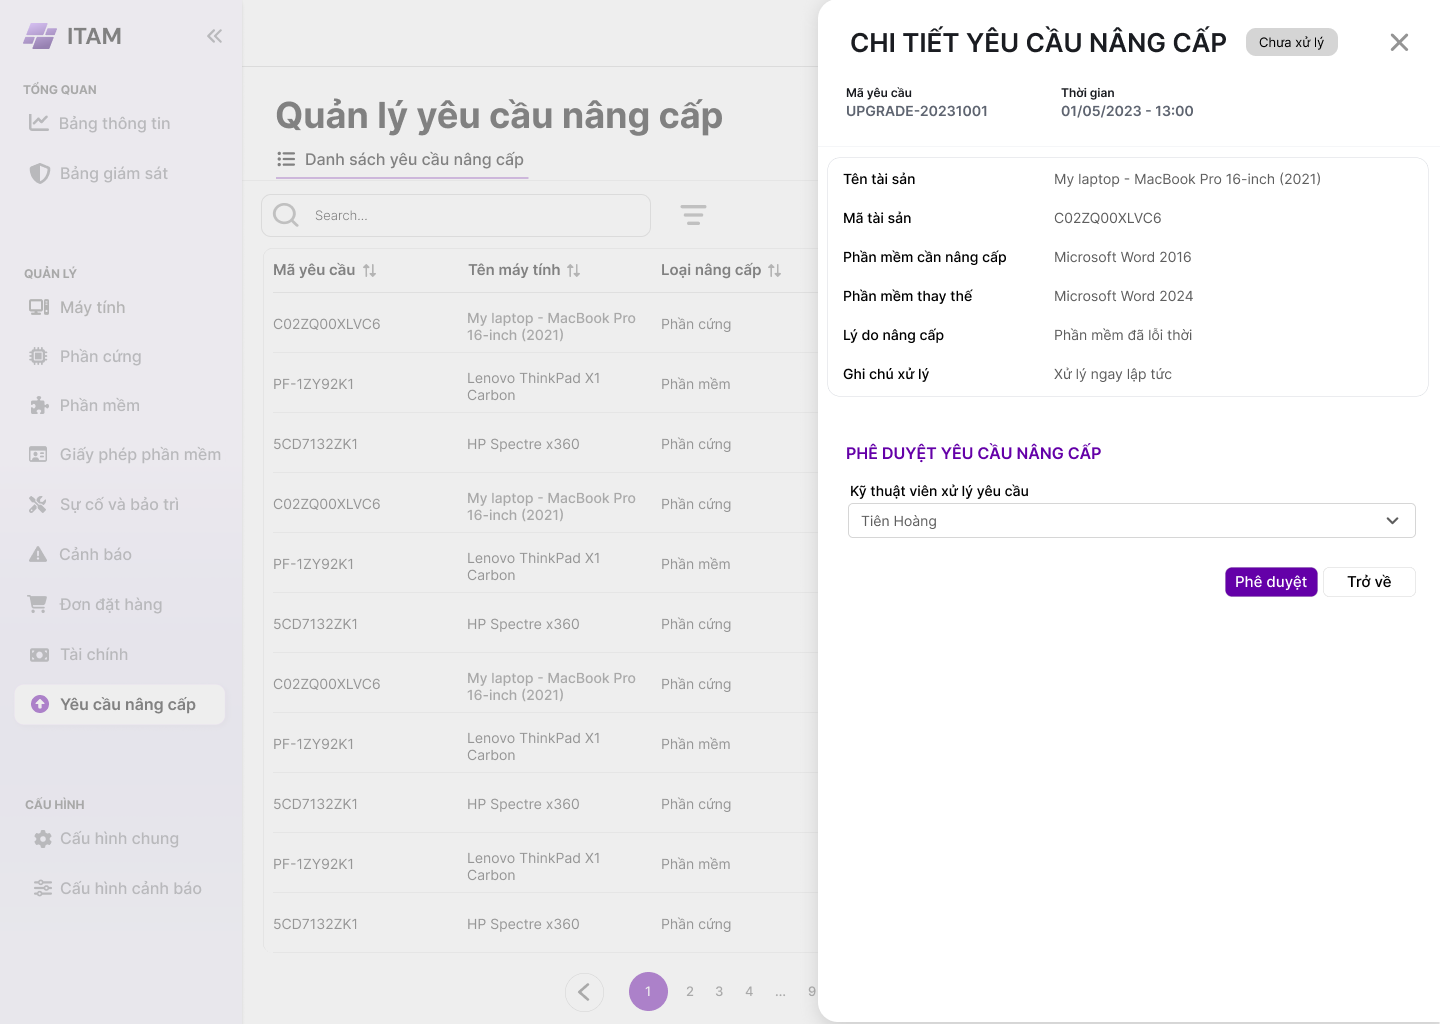
\includegraphics[width=14cm]{Images/C5/UI/Feature-Quản lý yêu cầu nâng cấp 2.4.png}
%     \vspace{15pt}
%     \caption{Giao diện Quản lý yêu cầu nâng cấp 2}
% \end{figure}

\item{Quản lý yêu cầu thanh lý}\\
Người dùng có thể xem danh sách các yêu cầu thanh lý và chi tiết các yêu cầu thanh lý đó, đồng thời quản lý cũng có thể phê duyệt các yêu cầu thanh lý (xem thêm chi tiết ở phụ lục).

\item{Quản lý đơn đặt hàng}\\
Người dùng với vai trò quản lý có thể xem danh sách đơn đặt hàng và chi tiết đơn đặt hàng, tạo đơn đặt hàng mới (xem thêm chi tiết ở phụ lục).
% \begin{figure}[H]
%     \centering
%     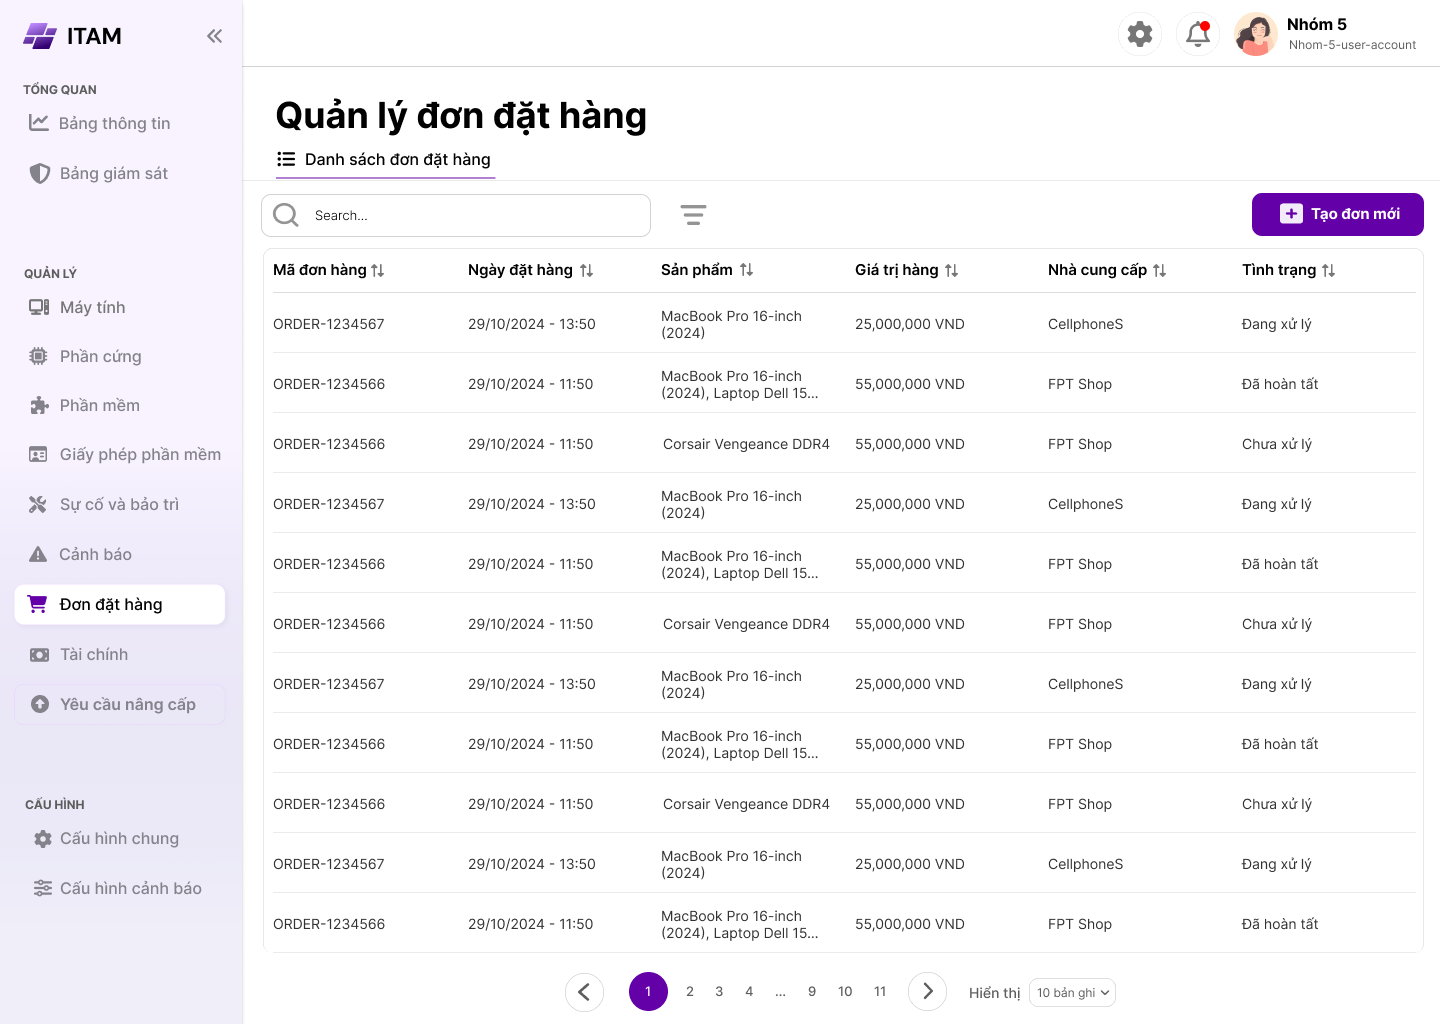
\includegraphics[width=14cm]{Images/C5/UI/Feature-Quản lý đơn đặt hàng 1.png}
%     \vspace{15pt}
%     \caption{Giao diện Quản lý đơn đặt hàng 1}
% \end{figure}
% \begin{figure}[H]
%     \centering
%     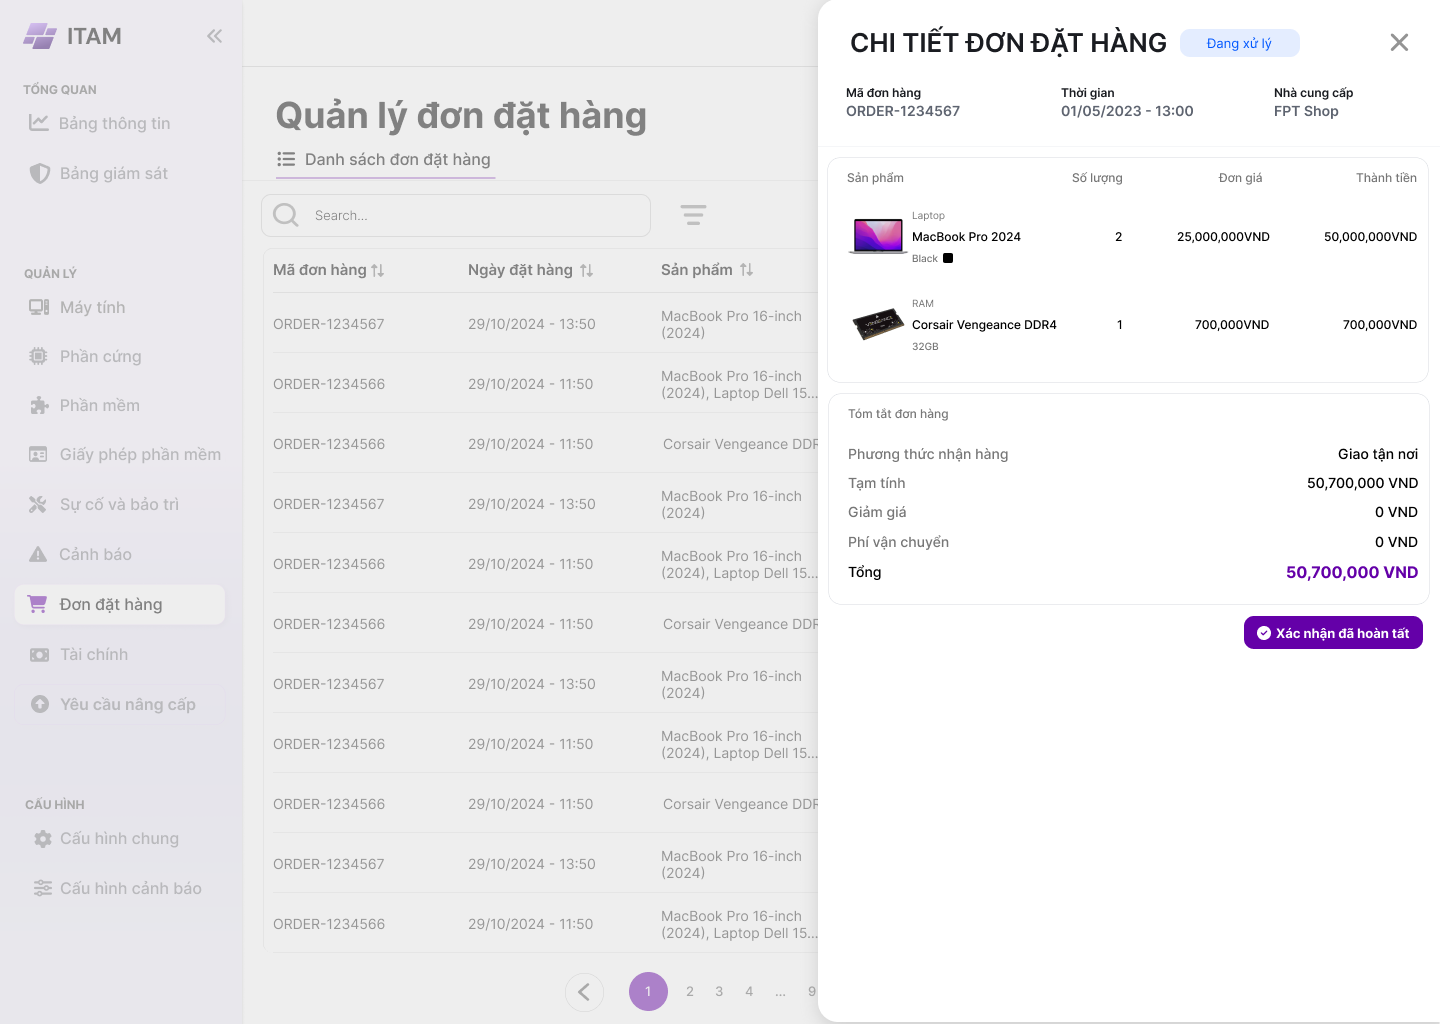
\includegraphics[width=14cm]{Images/C5/UI/Feature-Quản lý đơn đặt hàng 2.1.png}
%     \vspace{15pt}
%     \caption{Giao diện Quản lý đơn đặt hàng 2}
% \end{figure}
% \begin{figure}[H]
%     \centering
%     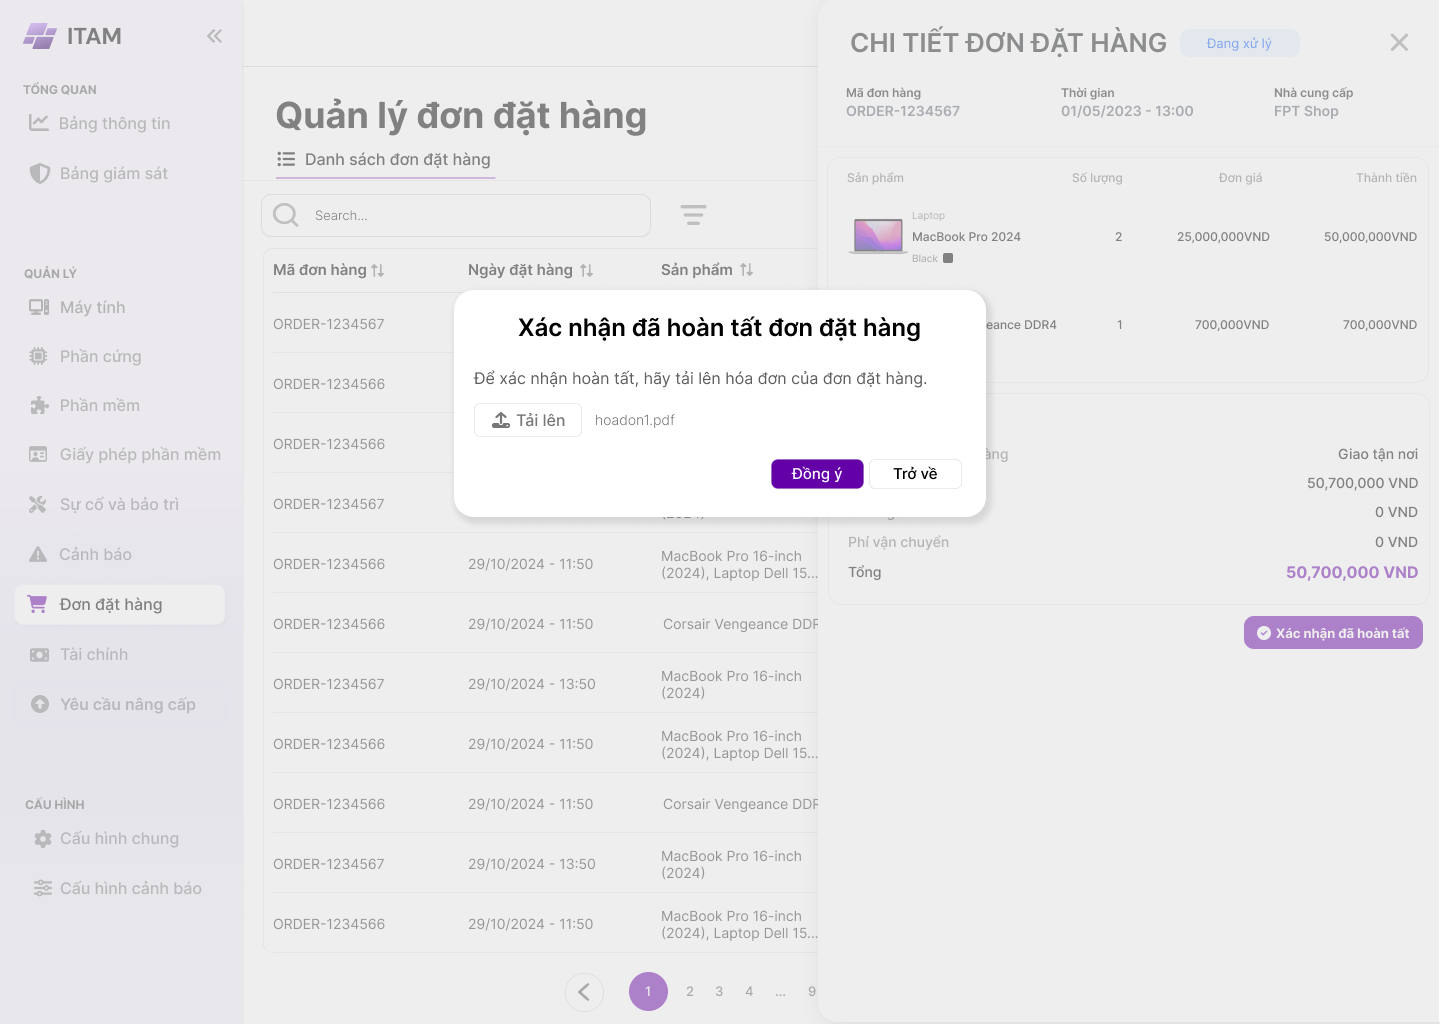
\includegraphics[width=14cm]{Images/C5/UI/Feature-Quản lý đơn đặt hàng 2.2.png}
%     \vspace{15pt}
%     \caption{Giao diện Quản lý đơn đặt hàng 3}
% \end{figure}
% \begin{figure}[H]
%     \centering
%     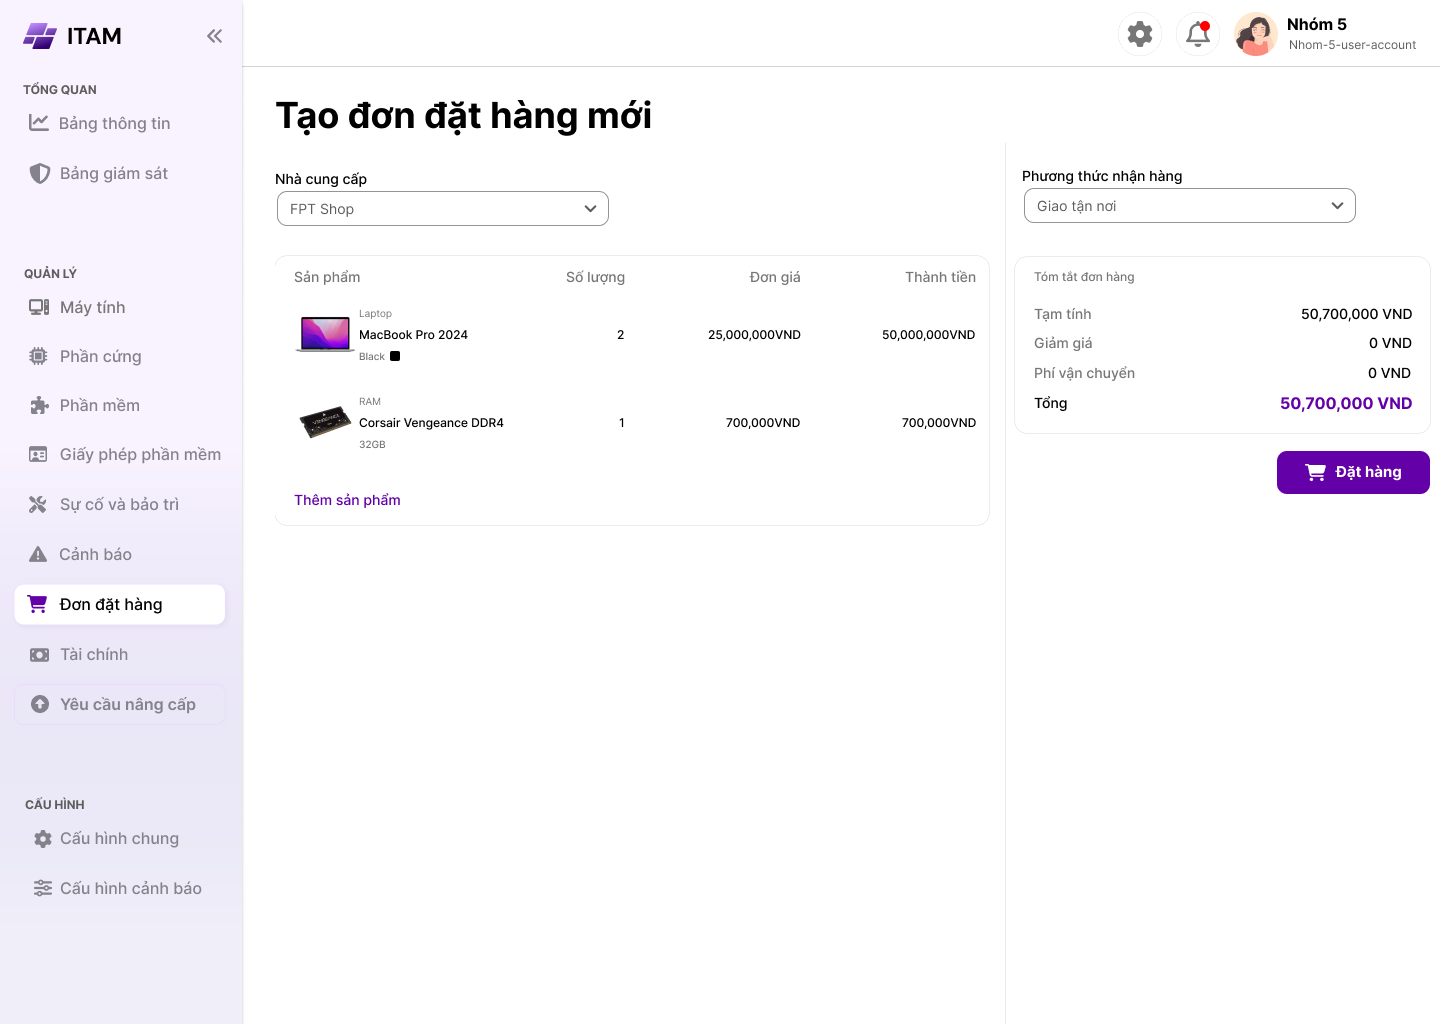
\includegraphics[width=14cm]{Images/C5/UI/Feature-Quản lý đơn đặt hàng 3.1.png}
%     \vspace{15pt}
%     \caption{Giao diện Quản lý đơn đặt hàng 3}
% \end{figure}
% \begin{figure}[H]
%     \centering
%     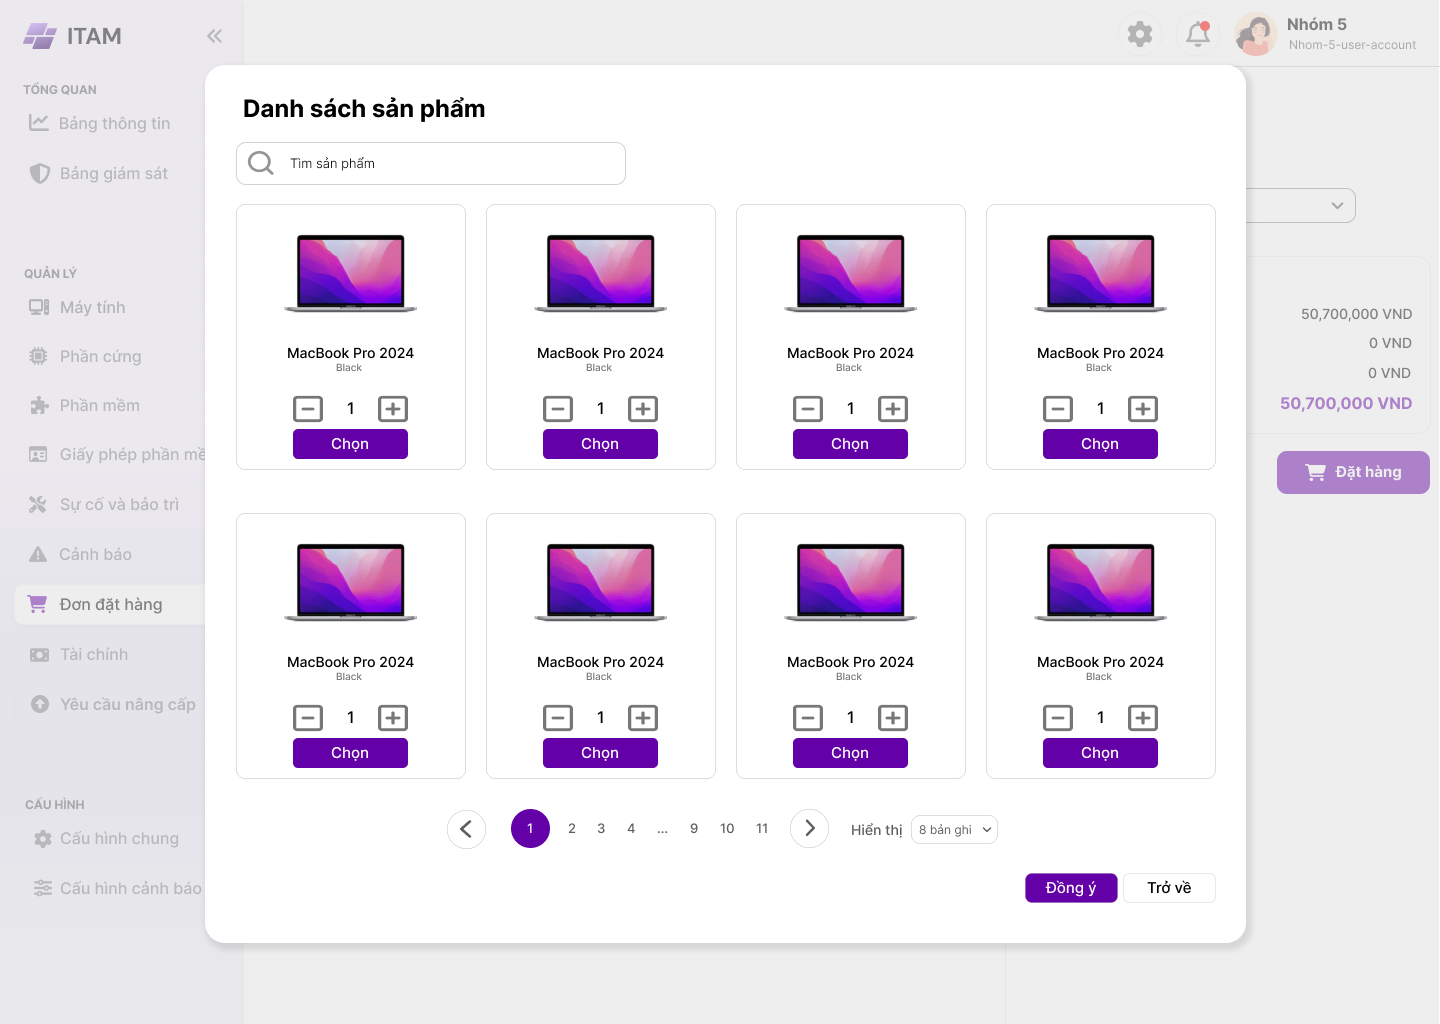
\includegraphics[width=14cm]{Images/C5/UI/Feature-Quản lý đơn đặt hàng 3.2.png}
%     \vspace{15pt}
%     \caption{Giao diện Quản lý đơn đặt hàng 5}
% \end{figure}
% \begin{figure}[H]
%     \centering
%     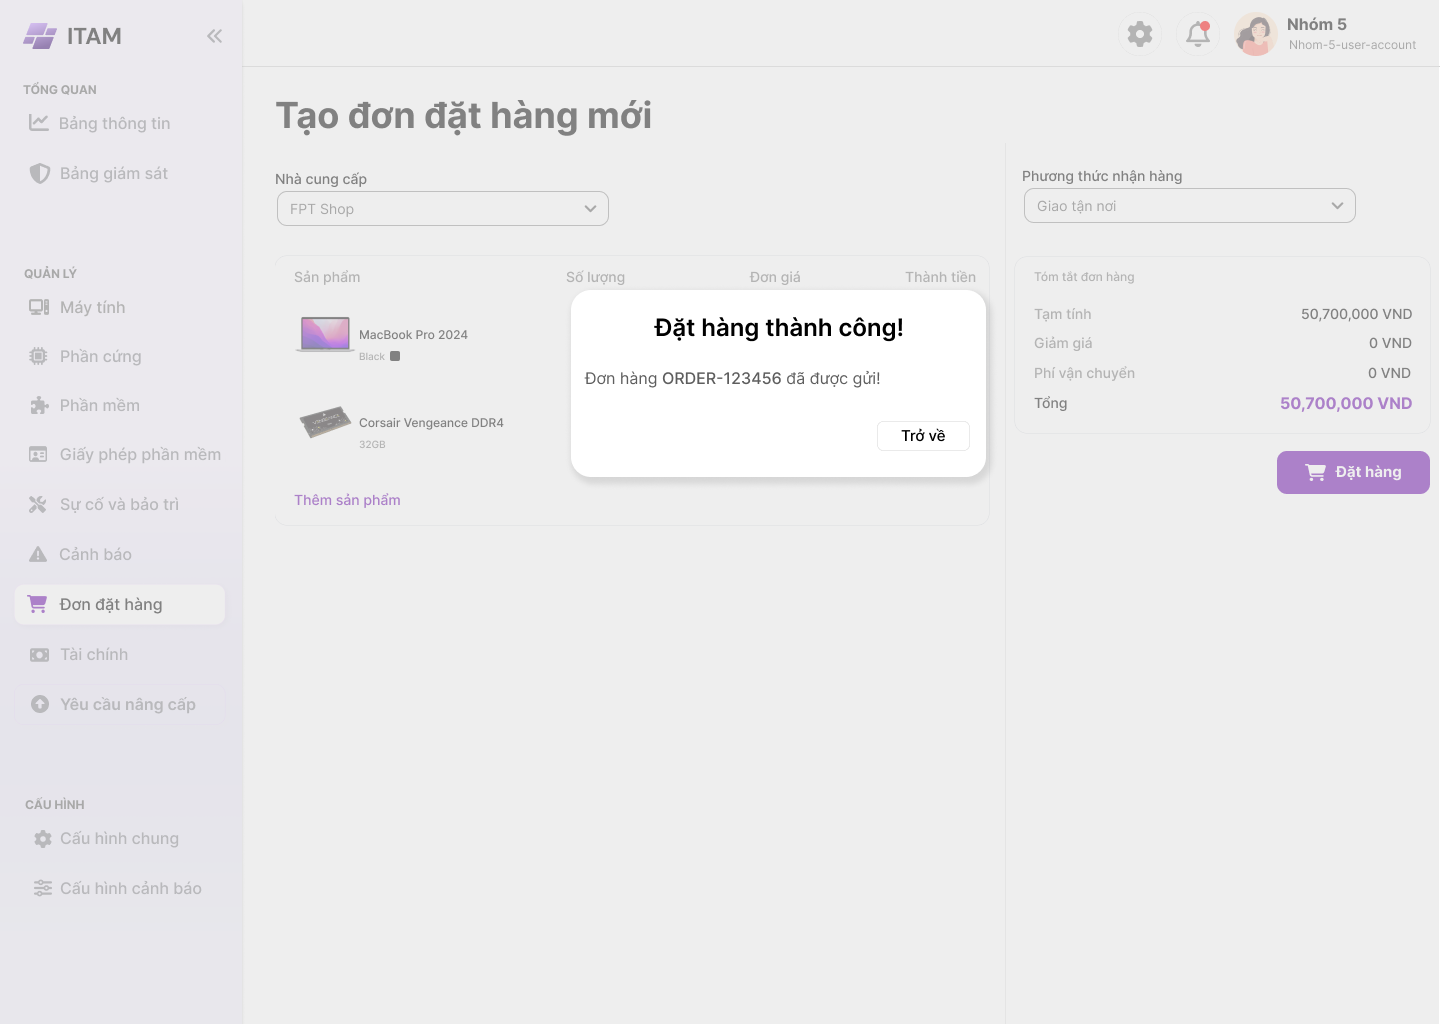
\includegraphics[width=14cm]{Images/C5/UI/Feature-Quản lý đơn đặt hàng 3.3.png}
%     \vspace{15pt}
%     \caption{Giao diện Quản lý đơn đặt hàng 6}
% \end{figure}

\item{Quản lý giấy phép phần mềm}\\
Quản lý giấy phép mềm hiển thị danh sách và thông tin của các giấy phép phần mềm có trong hệ thống (xem thêm chi tiết ở phụ lục).
% \begin{figure}[H]
%     \centering
%     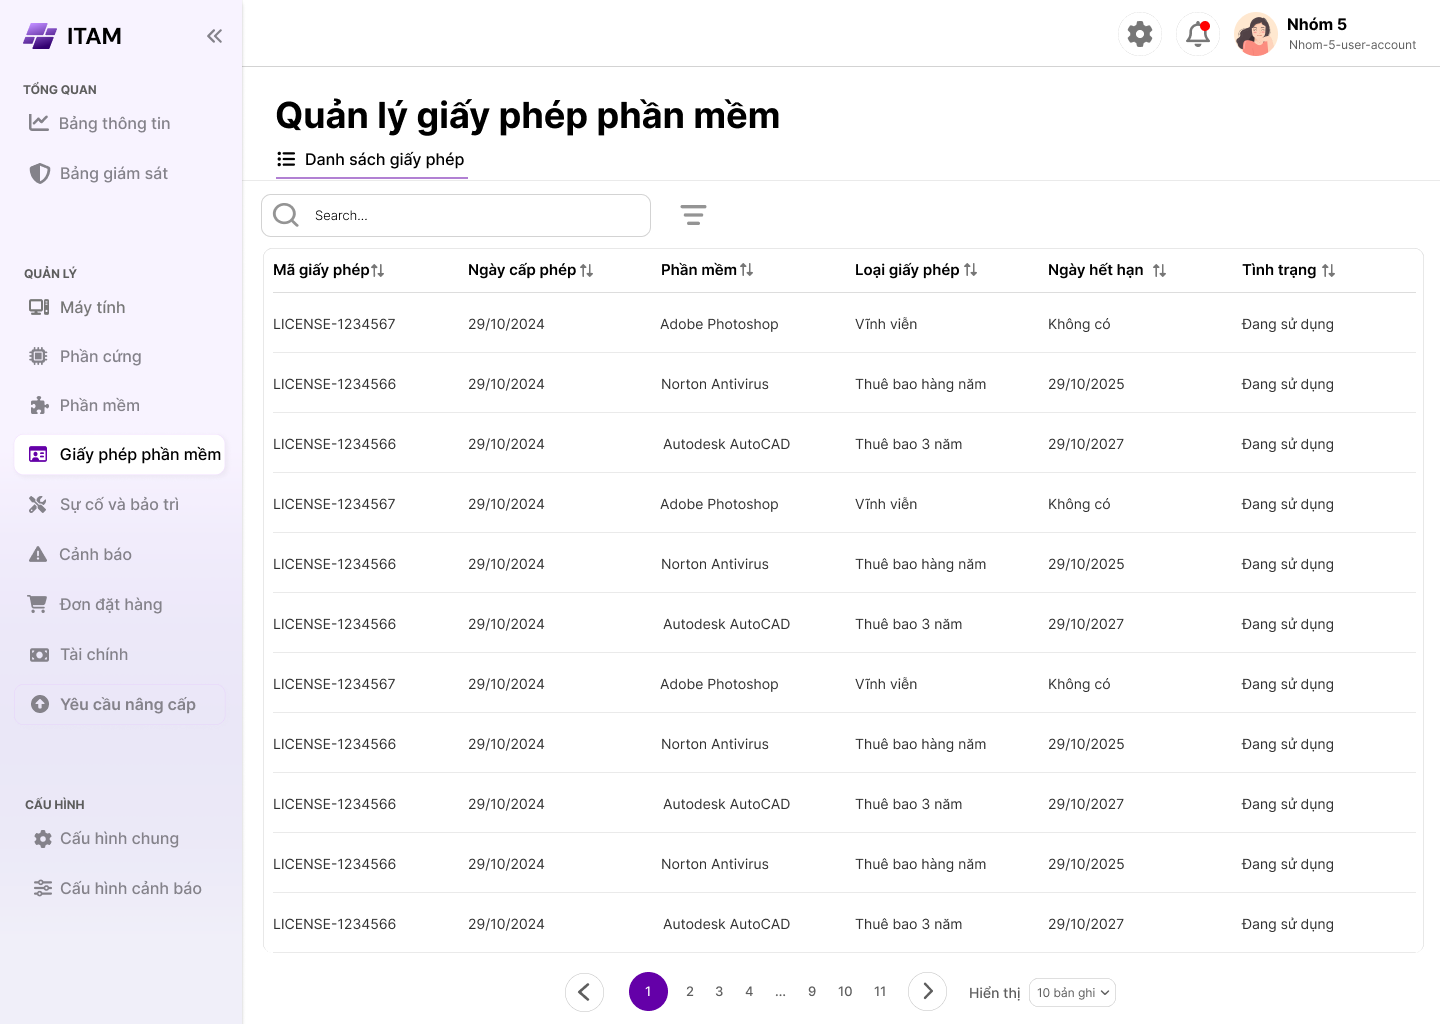
\includegraphics[width=14cm]{Images/C5/UI/Feature-Quản lý giấy phép phần mềm.png}
%     \vspace{15pt}
%     \caption{Giao diện Quản lý giấy phép phần mềm}
% \end{figure}

\item{Quản lý cấu hình cảnh báo}\\
Người dùng truy cập vào Cấu hình cảnh báo để điều chỉnh các ngưỡng của cảnh báo cho các máy tính trong hệ thống. Dựa vào các ngưỡng này, cảnh báo sẽ được sinh ra (xem thêm chi tiết ở phụ lục).
% \begin{figure}[H]
%     \centering
%     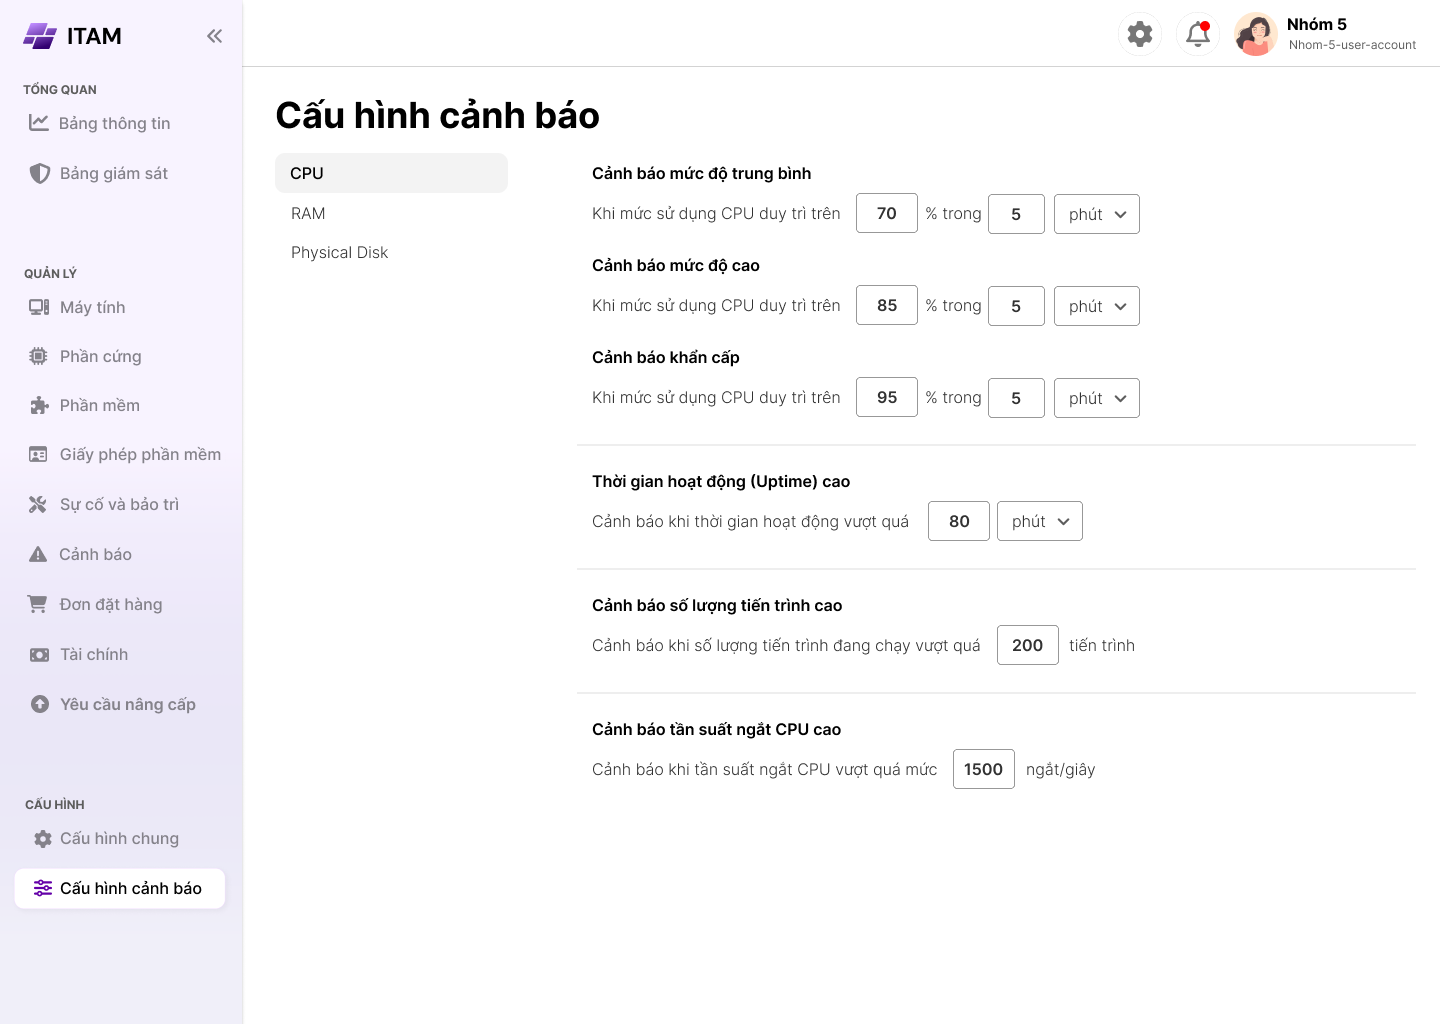
\includegraphics[width=14cm]{Images/C5/UI/Feature-Cấu hình cảnh báo 1.png}
%     \vspace{15pt}
%     \caption{Giao diện Quản lý cấu hình cảnh báo 1}
% \end{figure}
% \begin{figure}[H]
%     \centering
%     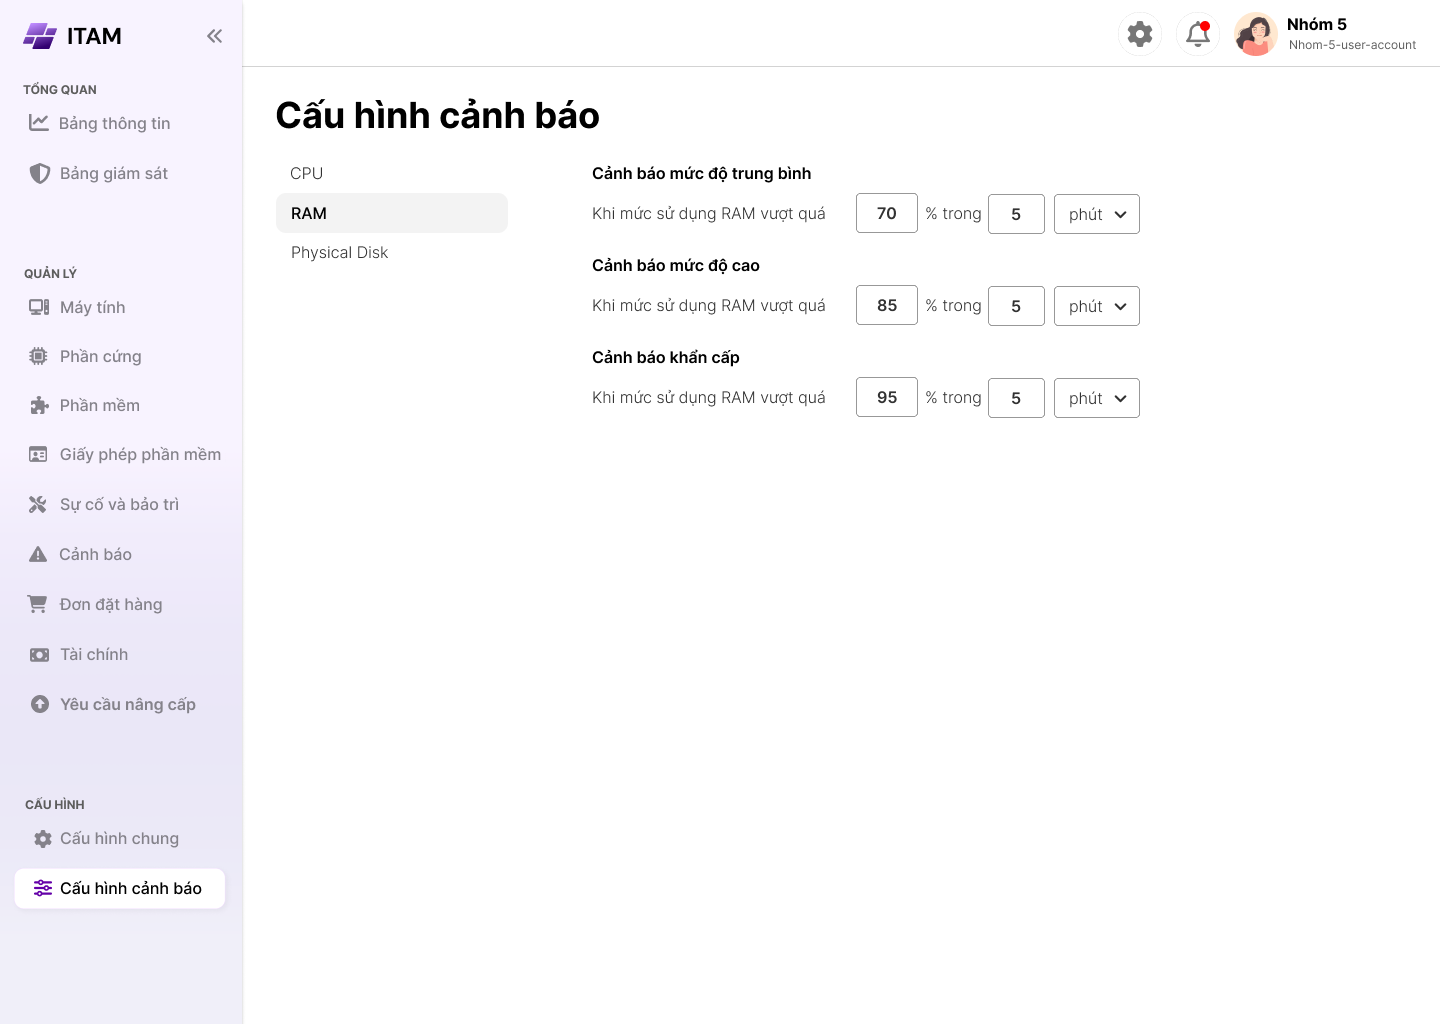
\includegraphics[width=14cm]{Images/C5/UI/Feature-Cấu hình cảnh báo 5.png}
%     \vspace{15pt}
%     \caption{Giao diện Quản lý cấu hình cảnh báo 2}
% \end{figure}
% \begin{figure}[H]
%     \centering
%     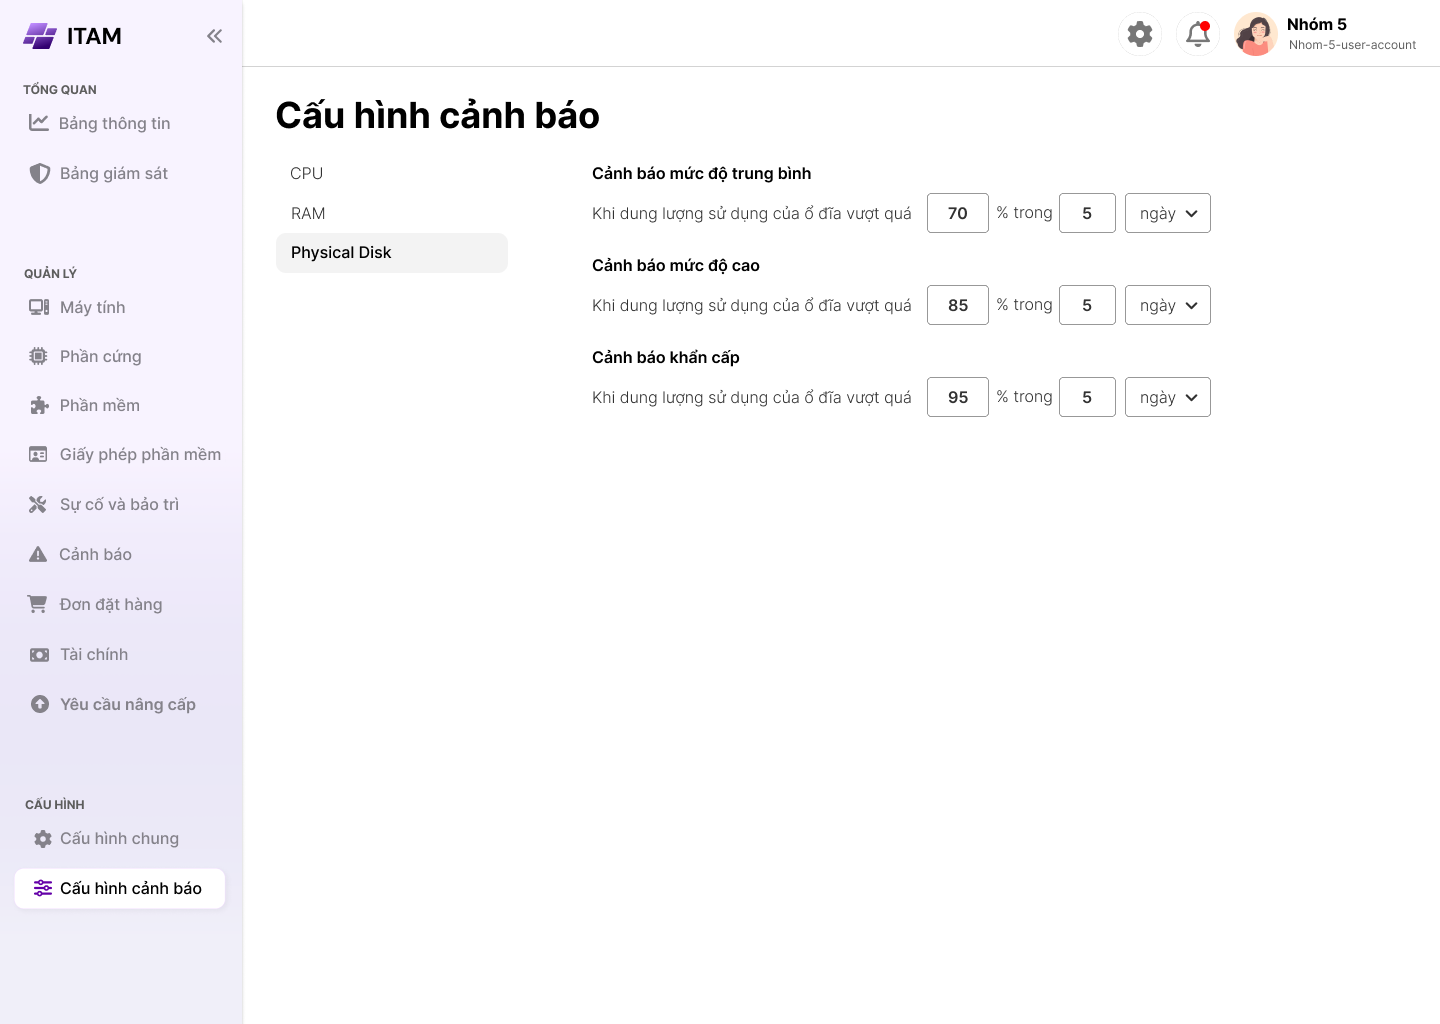
\includegraphics[width=14cm]{Images/C5/UI/Feature-Cấu hình cảnh báo 6.png}
%     \vspace{15pt}
%     \caption{Giao diện Quản lý cấu hình cảnh báo 3}
% \end{figure}

\end{itemize}
\subsection{Kết chương}
\noindent Trong quá trình phát triển một hệ thống hoàn chỉnh, phân tích và thiết kế đóng vai trò cốt lõi.
Chương này nhóm đã ba nội dung chính:
\begin{itemize}
    \item \textbf{Phân tích}: Mô hình hóa quy trình nghiệp vụ và các tương tác trong hệ thống.
    \item \textbf{Giải pháp công nghệ}: Đề xuất các giải pháp, đặc biệt là xử lý thời gian thực để đáp ứng yêu cầu nghiệp vụ.
    \item \textbf{Thiết kế}: Bao gồm thiết kế kiến trúc hệ thống, cơ sở dữ liệu, chi tiết bên trong và giao diện người dùng.
\end{itemize}
Qua phần phân tích nhóm đã đưa ra mô hình hóa nghiệp vụ cho các qui trình: giám sát tài sản, quản lý vòng đời tài sản, cảnh báo, quản lý đơn đặt hàng. Bên cạnh đó nhóm cũng đưa ra các use case cho hệ thống để trình bày các luồng thực thi cho hệ thống.\\ \\ 
Đến phần giải pháp công nghệ, nhóm đã trình bày các khái niệm, khía cạnh liên quan đến thu thập và xử lý dữ liệu thời gian thực. Ngoài ra nhóm cũng đã đi sâu vào phần công nghệ Kafka (công nghệ cốt lõi mà nhóm đã chọn) và so sánh Kafka với hai loại công nghệ khác là .\\ \\
Cuối cùng là phần thiết kế, trong phần này, nhóm đã đưa ra một kiến trúc hệ thống gồm 3 lớp là Presentation, Application, Storage. Từ đó nhóm đã lựa chọn các công nghệ cho Front-End là Angular và Back-end là ASP.NET Core, cơ sở dữ liệu là MSSQL. Nhóm cũng đã thiết kế ERD, làm rõ mối quan hệ giữa các đối tượng dữ liệu của hệ thống. Bên cạnh đó, nhóm cũng đã trình bày chi tiết bên trong qua class diagram và giao diện bên ngoài qua figma.



